\documentclass[oneside, letterpaper, 10pt, oldfontcommands]{memoir}
\usepackage{uwthesis}

\usepackage[caption=false]{subfig}
%\usepackage{subfigure}
\usepackage{graphicx}
\usepackage{bm}
\usepackage{amssymb}
\usepackage{amsmath}
\usepackage{amsfonts}
\usepackage[utf8]{inputenc}
\usepackage{placeins}
% defines table rules for professional looking tables
\usepackage{booktabs}
\usepackage{gensymb}
\usepackage[colorlinks=true,allcolors=blue]{hyperref}
\usepackage{microtype}
\usepackage{multirow, makecell}
\usepackage[capitalise]{cleveref}
\usepackage[utf8]{inputenc}
\usepackage{listings}
\usepackage{siunitx}
%\sisetup{detect-weight=true, detect-family=true}
\sisetup{detect-all = true}
\usepackage{xspace}
\usepackage{comment}
\usepackage{ragged2e}
\usepackage{lineno}

\newcommand{\Python}{\texttt{Python}}
\newcommand{\MCEq}{\texttt{MCE{\scriptsize Q}}}
\newcommand{\MMC}{\texttt{MMC}}
\newcommand{\PROPOSAL}{\texttt{PROPOSAL}}
\newcommand{\CORSIKA}{\texttt{CORSIKA}}
\newcommand{\MUONGUN}{\texttt{MUONGUN}}
\newcommand{\PHOTOSPLINE}{\texttt{PHOTOSPLINE}}
\newcommand{\like}{\mathcal{L}}
\newcommand{\likeSAY}{\mathcal{L}_{\textrm{Eff}}}
\newcommand{\pdfSxi}{S(\vec{x}_i)}
\newcommand{\TS}{\mathrm{TS}}
\newcommand{\Fermi}{\textit{Fermi}}
\newcommand{\nuveto}{{\LARGE $\nu$}\texttt{eto}}

\DeclareMathOperator*{\argmax}{arg\,max}
\DeclareMathOperator*{\argmin}{arg\,min}

\newcommand{\refeq}[1]{Eq.~(\ref{#1})}
\newcommand{\refeqs}[2]{Eqs.~(\ref{#1})~and~(\ref{#2})}
\newcommand{\refeqss}[3]{Eqs.~(\ref{#1}), (\ref{#2})~and~(\ref{#3})}
\newcommand{\reffig}[1]{Fig.~\ref{#1}}
\newcommand{\reffigs}[2]{Figs.~\ref{#1}~and~\ref{#2}}
\newcommand{\refsec}[1]{Section~\ref{#1}}
\newcommand{\refsecs}[5]{Sections~\ref{#1},~\ref{#2},~\ref{#3},~\ref{#4},~and~\ref{#5}}
\newcommand{\refappsec}[1]{Appendix Section~\ref{#1}}
\newcommand{\refapp}[1]{Appendix~\ref{#1}}
\newcommand{\reftab}[1]{Table~\ref{#1}}
\newcommand{\refref}[1]{Ref.~\cite{#1}}
\newcommand{\refrefs}[2]{Refs.~\cite{#1}~and~\cite{#2}}

% This holds definitions of macros to enforce consistency in units.

% This file is the sole location for such definitions.  Check here to
% learn what there is and add new ones only here.

% also see defs.tex for names.


% see
%  http://ctan.org/pkg/siunitx
%  http://mirrors.ctan.org/macros/latex/contrib/siunitx/siunitx.pdf

% Examples:
%  % angles
%  \ang{1.5} off-axis
%
%  % just a unit
%  \si{\kilo\tonne}
%
%  % with a value:
%  \SI{10}{\mega\electronvolt}

%  range of values:
% \SIrange{60}{120}{\GeV}

% some shorthand notation
%\DeclareSIUnit \MBq {\mega\Bq}
\DeclareSIUnit \s {\second}
\DeclareSIUnit \ns {\nano\second}
\DeclareSIUnit \mus {\micro\second}
\DeclareSIUnit \ms {\milli\second}
\DeclareSIUnit \MB {\mega\byte}
\DeclareSIUnit \GB {\giga\byte}
\DeclareSIUnit \TB {\tera\byte}
\DeclareSIUnit \PB {\peta\byte}
\DeclareSIUnit \Mbps {\mega\bit/\s}
\DeclareSIUnit \Gbps {\giga\bit/\s}
\DeclareSIUnit \Tbps {\tera\bit/\s}
\DeclareSIUnit \Pbps {\peta\bit/\s}
\DeclareSIUnit \kton {\kilo\tonne} % changed  back to kton
\DeclareSIUnit \kt {\kilo\tonne}
\DeclareSIUnit \Mt {\mega\tonne}
\DeclareSIUnit \eV {\electronvolt}
\DeclareSIUnit \keV {\kilo\electronvolt}
\DeclareSIUnit \MeV {\mega\electronvolt}
\DeclareSIUnit \GeV {\giga\electronvolt}
\DeclareSIUnit \PeV {\peta\electronvolt}
\DeclareSIUnit \EeV {\exa\electronvolt}
\DeclareSIUnit \m {\meter}
\DeclareSIUnit \cm {\centi\meter}
\DeclareSIUnit \in {\inchcommand}
\DeclareSIUnit \km {\kilo\meter}
\DeclareSIUnit \kV {\kilo\volt}
\DeclareSIUnit \kW {\kilo\watt}
\DeclareSIUnit \MW {\mega\watt}
\DeclareSIUnit \MHz {\mega\hertz}
\DeclareSIUnit \mrad {\milli\radian}
\DeclareSIUnit \year {years}
\DeclareSIUnit \POT {POT}
\DeclareSIUnit \sig {$\sigma$}
\DeclareSIUnit\parsec{pc}
\DeclareSIUnit\lightyear{ly}
\DeclareSIUnit\foot{ft}
\DeclareSIUnit\ft{ft}
\DeclareSIUnit \ppb{ppb}
\DeclareSIUnit \ppt{ppt}
\DeclareSIUnit \samples{S}
\DeclareSIUnit \pe{PE}
\DeclareSIUnit \sr{\steradian}

\newcommand\SigmaOne{\SI{68.3}\percent}
\newcommand\SigmaTwo{\SI{95.4}\percent}

% "the Glashow Resonance energy"
\newcommand\GlashowEnergy{\SI{6.3}\PeV\xspace}
%

% The reconstructed deposited energy cut
\newcommand\EnergyCut{\SI{60}\TeV\xspace}

% The sample livetime
\newcommand\Livetime{\SI{7.5}\year\xspace}

% The segmented power law
\newcommand\minunfoldingenergy{1.995\times10^4}
\newcommand\maxunfoldingenergy{3.162\times10^8}
\newcommand\unfoldingsegments{13}

% Analysis parameters
\newcommand\astronorm{\Phi_\texttt{astro}}
\newcommand\astrodeltagamma{\gamma_\texttt{astro}}
\newcommand\convnorm{\Phi_\texttt{conv}}
\newcommand\promptnorm{\Phi_\texttt{prompt}}
\newcommand\pik{R_{K/\pi}}
\newcommand\atmonunubar{{2\nu/\left(\nu+\bar{\nu}\right)}_\texttt{atmo}}
\newcommand\crdeltagamma{\Delta\gamma_\texttt{CR}}
\newcommand\muonnorm{\Phi_\mu}
\newcommand\domeff{\epsilon_\texttt{DOM}}
\newcommand\holeice{\epsilon_\texttt{head-on}}
\newcommand\anisotropy{a_s}

% Parameters not in the analysis



\usepackage{xparse}

\ExplSyntaxOn
\DeclareExpandableDocumentCommand{\eval}{m}{\fp_eval:n {#1}}
\ExplSyntaxOff


% SPL Frequentist Wilks results
\newcommand\SPLFreqBFCRDeltaGamma{-0.053}
\newcommand\SPLFreqWilksUpperCRDeltaGamma{-0.006}
\newcommand\SPLFreqWilksLowerCRDeltaGamma{-0.184}
\newcommand\SPLFreqWilksUpperCRDeltaGammaDelta{0.048}
\newcommand\SPLFreqWilksLowerCRDeltaGammaDelta{0.131}
\newcommand\SPLFreqWilksCRDeltaGammaSummary{-0.053^{+0.048}_{-0.131}}
\newcommand\SPLFreqBFAtmoNuRatio{1.002}
\newcommand\SPLFreqWilksUpperAtmoNuRatio{1.102}
\newcommand\SPLFreqWilksLowerAtmoNuRatio{0.902}
\newcommand\SPLFreqWilksUpperAtmoNuRatioDelta{0.100}
\newcommand\SPLFreqWilksLowerAtmoNuRatioDelta{0.100}
\newcommand\SPLFreqWilksAtmoNuRatioSummary{1.002^{+0.100}_{-0.100}}
\newcommand\SPLFreqBFAniScale{1.00}
\newcommand\SPLFreqWilksUpperAniScale{1.20}
\newcommand\SPLFreqWilksLowerAniScale{0.80}
\newcommand\SPLFreqWilksUpperAniScaleDelta{0.20}
\newcommand\SPLFreqWilksLowerAniScaleDelta{0.20}
\newcommand\SPLFreqWilksAniScaleSummary{1.00^{+0.20}_{-0.20}}
\newcommand\SPLFreqBFIndex{2.88}
\newcommand\SPLFreqWilksUpperIndex{3.08}
\newcommand\SPLFreqWilksLowerIndex{2.69}
\newcommand\SPLFreqWilksUpperIndexDelta{0.20}
\newcommand\SPLFreqWilksLowerIndexDelta{0.19}
\newcommand\SPLFreqWilksIndexSummary{2.88^{+0.20}_{-0.19}}
\newcommand\SPLFreqBFNorm{6.44}
\newcommand\SPLFreqWilksUpperNorm{7.92}
\newcommand\SPLFreqWilksLowerNorm{4.85}
\newcommand\SPLFreqWilksUpperNormDelta{1.48}
\newcommand\SPLFreqWilksLowerNormDelta{1.60}
\newcommand\SPLFreqWilksNormSummary{6.44^{+1.48}_{-1.60}}
\newcommand\SPLFreqBFConvNorm{1.01}
\newcommand\SPLFreqWilksUpperConvNorm{1.36}
\newcommand\SPLFreqWilksLowerConvNorm{0.67}
\newcommand\SPLFreqWilksUpperConvNormDelta{0.35}
\newcommand\SPLFreqWilksLowerConvNormDelta{0.33}
\newcommand\SPLFreqWilksConvNormSummary{1.01^{+0.35}_{-0.33}}
\newcommand\SPLFreqBFDOMEff{0.951}
\newcommand\SPLFreqWilksUpperDOMEff{1.041}
\newcommand\SPLFreqWilksLowerDOMEff{0.884}
\newcommand\SPLFreqWilksUpperDOMEffDelta{0.090}
\newcommand\SPLFreqWilksLowerDOMEffDelta{0.067}
\newcommand\SPLFreqWilksDOMEffSummary{0.951^{+0.090}_{-0.067}}
\newcommand\SPLFreqBFHoleIce{-0.06}
\newcommand\SPLFreqWilksUpperHoleIce{0.45}
\newcommand\SPLFreqWilksLowerHoleIce{-0.54}
\newcommand\SPLFreqWilksUpperHoleIceDelta{0.51}
\newcommand\SPLFreqWilksLowerHoleIceDelta{0.48}
\newcommand\SPLFreqWilksHoleIceSummary{-0.06^{+0.51}_{-0.48}}
\newcommand\SPLFreqBFMuonNorm{1.21}
\newcommand\SPLFreqWilksUpperMuonNorm{1.67}
\newcommand\SPLFreqWilksLowerMuonNorm{0.75}
\newcommand\SPLFreqWilksUpperMuonNormDelta{0.46}
\newcommand\SPLFreqWilksLowerMuonNormDelta{0.46}
\newcommand\SPLFreqWilksMuonNormSummary{1.21^{+0.46}_{-0.46}}
\newcommand\SPLFreqBFKPi{1.000}
\newcommand\SPLFreqWilksUpperKPi{1.100}
\newcommand\SPLFreqWilksLowerKPi{0.901}
\newcommand\SPLFreqWilksUpperKPiDelta{0.100}
\newcommand\SPLFreqWilksLowerKPiDelta{0.099}
\newcommand\SPLFreqWilksKPiSummary{1.000^{+0.100}_{-0.099}}
\newcommand\SPLFreqBFPromptNorm{0.00}
\newcommand\SPLFreqWilksUpperPromptNorm{5.17}
\newcommand\SPLFreqWilksLowerPromptNorm{0.00}
\newcommand\SPLFreqWilksUpperPromptNormDelta{5.17}
\newcommand\SPLFreqWilksLowerPromptNormDelta{0.00}
\newcommand\SPLFreqWilksPromptNormSummary{0.00^{+5.17}_{-0.00}}

% prompt normalization
\newcommand\NoAstroPromptNorm{25.7} %25.65
\newcommand\ICFiftyNinePromptUpperLimit{3.80} % ERS at 90 % CL
\newcommand\SPLFreqWilksNinetyUpperLimit{9.65}

% prompt bayes factor
\newcommand\BayesFactorSubstantialPromptNorm{8.65}
\newcommand\BayesFactorStrongPromptNorm{13.21}
\newcommand\BayesFactorVeryStrongPromptNorm{17.18}
\newcommand\BayesFactorDecisivePromptNorm{21.16}

% SPL Bayesian HPD results

\newcommand\SPLBayesMAPCRDeltaGamma{-0.039}
\newcommand\SPLBayesHPDUpperCRDeltaGamma{0.009}
\newcommand\SPLBayesHPDLowerCRDeltaGamma{-0.086}
\newcommand\SPLBayesHPDUpperCRDeltaGammaDelta{0.048}
\newcommand\SPLBayesHPDLowerCRDeltaGammaDelta{0.047}
\newcommand\SPLBayesCRDeltaGammaSummary{-0.039^{+0.048}_{-0.047}}\newcommand\SPLBayesMAPAtmoNuRatio{1.010}
\newcommand\SPLBayesHPDUpperAtmoNuRatio{1.101}
\newcommand\SPLBayesHPDLowerAtmoNuRatio{0.906}
\newcommand\SPLBayesHPDUpperAtmoNuRatioDelta{0.091}
\newcommand\SPLBayesHPDLowerAtmoNuRatioDelta{0.105}
\newcommand\SPLBayesAtmoNuRatioSummary{1.010^{+0.091}_{-0.105}}\newcommand\SPLBayesMAPAniScale{0.97}
\newcommand\SPLBayesHPDUpperAniScale{1.19}
\newcommand\SPLBayesHPDLowerAniScale{0.79}
\newcommand\SPLBayesHPDUpperAniScaleDelta{0.22}
\newcommand\SPLBayesHPDLowerAniScaleDelta{0.18}
\newcommand\SPLBayesAniScaleSummary{0.97^{+0.22}_{-0.18}}\newcommand\SPLBayesMAPIndex{2.85}
\newcommand\SPLBayesHPDUpperIndex{3.10}
\newcommand\SPLBayesHPDLowerIndex{2.68}
\newcommand\SPLBayesHPDUpperIndexDelta{0.26}
\newcommand\SPLBayesHPDLowerIndexDelta{0.17}
\newcommand\SPLBayesIndexSummary{2.85^{+0.26}_{-0.17}}\newcommand\SPLBayesMAPNorm{5.63}
\newcommand\SPLBayesHPDUpperNorm{7.14}
\newcommand\SPLBayesHPDLowerNorm{4.10}
\newcommand\SPLBayesHPDUpperNormDelta{1.52}
\newcommand\SPLBayesHPDLowerNormDelta{1.52}
\newcommand\SPLBayesNormSummary{5.63^{+1.52}_{-1.52}}\newcommand\SPLBayesMAPConvNorm{0.98}
\newcommand\SPLBayesHPDUpperConvNorm{1.28}
\newcommand\SPLBayesHPDLowerConvNorm{0.58}
\newcommand\SPLBayesHPDUpperConvNormDelta{0.31}
\newcommand\SPLBayesHPDLowerConvNormDelta{0.40}
\newcommand\SPLBayesConvNormSummary{0.98^{+0.31}_{-0.40}}\newcommand\SPLBayesMAPDOMEff{0.933}
\newcommand\SPLBayesHPDUpperDOMEff{1.007}
\newcommand\SPLBayesHPDLowerDOMEff{0.853}
\newcommand\SPLBayesHPDUpperDOMEffDelta{0.074}
\newcommand\SPLBayesHPDLowerDOMEffDelta{0.080}
\newcommand\SPLBayesDOMEffSummary{0.933^{+0.074}_{-0.080}}\newcommand\SPLBayesMAPHoleIce{-0.05}
\newcommand\SPLBayesHPDUpperHoleIce{0.44}
\newcommand\SPLBayesHPDLowerHoleIce{-0.61}
\newcommand\SPLBayesHPDUpperHoleIceDelta{0.49}
\newcommand\SPLBayesHPDLowerHoleIceDelta{0.56}
\newcommand\SPLBayesHoleIceSummary{-0.05^{+0.49}_{-0.56}}\newcommand\SPLBayesMAPMuonNorm{1.17}
\newcommand\SPLBayesHPDUpperMuonNorm{1.67}
\newcommand\SPLBayesHPDLowerMuonNorm{0.75}
\newcommand\SPLBayesHPDUpperMuonNormDelta{0.50}
\newcommand\SPLBayesHPDLowerMuonNormDelta{0.42}
\newcommand\SPLBayesMuonNormSummary{1.17^{+0.50}_{-0.42}}\newcommand\SPLBayesMAPKPi{1.011}
\newcommand\SPLBayesHPDUpperKPi{1.097}
\newcommand\SPLBayesHPDLowerKPi{0.897}
\newcommand\SPLBayesHPDUpperKPiDelta{0.086}
\newcommand\SPLBayesHPDLowerKPiDelta{0.114}
\newcommand\SPLBayesKPiSummary{1.011^{+0.086}_{-0.114}}\newcommand\SPLBayesMAPPromptNorm{0.18}
\newcommand\SPLBayesHPDUpperPromptNorm{5.97}
\newcommand\SPLBayesHPDLowerPromptNorm{0.00}
\newcommand\SPLBayesHPDUpperPromptNormDelta{5.79}
\newcommand\SPLBayesHPDLowerPromptNormDelta{0.18}
\newcommand\SPLBayesPromptNormSummary{0.18^{+5.79}_{-0.18}}

\newcommand\SPL{Single Power Law}
\newcommand\SPLBayes{0.0872}
\newcommand\SPLSPLBayes{2.53\times10^{63}}
\newcommand\SPLSPLPhiLower{-}
\newcommand\SPLSPLPhiMode{-}
\newcommand\SPLSPLPhiUpper{-}
\newcommand\SPLSPLPhiSummary{-}
\newcommand\SPLSPLGammaLower{-}
\newcommand\SPLSPLGammaMode{-}
\newcommand\SPLSPLGammaUpper{-}
\newcommand\SPLSPLGammaSummary{-}
\newcommand\SPLTableSummary{Generic & \SPL & $\SPLBayes$ & $\SPLSPLBayes$ & $\SPLSPLGammaSummary$ & $\SPLSPLPhiSummary$}
\newcommand\DPL{Double Power Law}
\newcommand\DPLBayes{1.93\times10^{-3}}
\newcommand\DPLSPLBayes{2.53\times10^{63}}
\newcommand\DPLSPLPhiLower{-}
\newcommand\DPLSPLPhiMode{-}
\newcommand\DPLSPLPhiUpper{-}
\newcommand\DPLSPLPhiSummary{-}
\newcommand\DPLSPLGammaLower{-}
\newcommand\DPLSPLGammaMode{-}
\newcommand\DPLSPLGammaUpper{-}
\newcommand\DPLSPLGammaSummary{-}
\newcommand\DPLTableSummary{Generic & \DPL & $\DPLBayes$ & $\DPLSPLBayes$ & $\DPLSPLGammaSummary$ & $\DPLSPLPhiSummary$}
\newcommand\LP{Log Parabola}
\newcommand\LPBayes{2.05\times10^{-3}}
\newcommand\LPSPLBayes{2.53\times10^{63}}
\newcommand\LPSPLPhiLower{-}
\newcommand\LPSPLPhiMode{-}
\newcommand\LPSPLPhiUpper{-}
\newcommand\LPSPLPhiSummary{-}
\newcommand\LPSPLGammaLower{-}
\newcommand\LPSPLGammaMode{-}
\newcommand\LPSPLGammaUpper{-}
\newcommand\LPSPLGammaSummary{-}
\newcommand\LPTableSummary{Generic & \LP & $\LPBayes$ & $\LPSPLBayes$ & $\LPSPLGammaSummary$ & $\LPSPLPhiSummary$}
\newcommand\Stecker{Stecker~\cite{Stecker:2013fxa}}
\newcommand\SteckerBayes{4.32\times10^{-13}}
\newcommand\SteckerSPLBayes{1.45\times10^{-10}}
\newcommand\SteckerSPLPhiLower{2.95}
\newcommand\SteckerSPLPhiMode{4.08}
\newcommand\SteckerSPLPhiUpper{5.88}
\newcommand\SteckerSPLPhiLowerDelta{\eval{\SteckerSPLPhiMode - \SteckerSPLPhiLower}}
\newcommand\SteckerSPLPhiUpperDelta{\eval{\SteckerSPLPhiUpper - \SteckerSPLPhiMode}}
\newcommand\SteckerSPLPhiSummary{\SteckerSPLPhiMode^{+\SteckerSPLPhiUpperDelta}_{-\SteckerSPLPhiLowerDelta}}
\newcommand\SteckerSPLGammaLower{3.5}
\newcommand\SteckerSPLGammaMode{3.97}
\newcommand\SteckerSPLGammaUpper{4.51}
\newcommand\SteckerSPLGammaLowerDelta{\eval{\SteckerSPLGammaMode - \SteckerSPLGammaLower}}
\newcommand\SteckerSPLGammaUpperDelta{\eval{\SteckerSPLGammaUpper - \SteckerSPLGammaMode}}
\newcommand\SteckerSPLGammaSummary{\SteckerSPLGammaMode^{+\SteckerSPLGammaUpperDelta}_{-\SteckerSPLGammaLowerDelta}}
\newcommand\SteckerTableSummary{AGN core & \Stecker & $\SteckerBayes$ & $\SteckerSPLBayes$ & $\SteckerSPLGammaSummary$ & $\SteckerSPLPhiSummary$}
\newcommand\Fang{Fang et al.~\cite{Fang:2017zjf}}
\newcommand\FangBayes{0.281}
\newcommand\FangSPLBayes{0.248}
\newcommand\FangSPLPhiLower{1.12}
\newcommand\FangSPLPhiMode{2.56}
\newcommand\FangSPLPhiUpper{3.84}
\newcommand\FangSPLPhiLowerDelta{\eval{\FangSPLPhiMode - \FangSPLPhiLower}}
\newcommand\FangSPLPhiUpperDelta{\eval{\FangSPLPhiUpper - \FangSPLPhiMode}}
\newcommand\FangSPLPhiSummary{\FangSPLPhiMode^{+\FangSPLPhiUpperDelta}_{-\FangSPLPhiLowerDelta}}
\newcommand\FangSPLGammaLower{3.33}
\newcommand\FangSPLGammaMode{3.83}
\newcommand\FangSPLGammaUpper{4.64}
\newcommand\FangSPLGammaLowerDelta{\eval{\FangSPLGammaMode - \FangSPLGammaLower}}
\newcommand\FangSPLGammaUpperDelta{\eval{\FangSPLGammaUpper - \FangSPLGammaMode}}
\newcommand\FangSPLGammaSummary{\FangSPLGammaMode^{+\FangSPLGammaUpperDelta}_{-\FangSPLGammaLowerDelta}}
\newcommand\FangTableSummary{AGN & \Fang & $\FangBayes$ & $\FangSPLBayes$ & $\FangSPLGammaSummary$ & $\FangSPLPhiSummary$}
\newcommand\KimuraBOne{Kimura et al. (B1)~\cite{Kimura:2014jba}}
\newcommand\KimuraBOneBayes{4.84\times10^{-6}}
\newcommand\KimuraBOneSPLBayes{8.38\times10^{-7}}
\newcommand\KimuraBOneSPLPhiLower{0.0}
\newcommand\KimuraBOneSPLPhiMode{0.98}
\newcommand\KimuraBOneSPLPhiUpper{2.02}
\newcommand\KimuraBOneSPLPhiLowerDelta{\eval{\KimuraBOneSPLPhiMode - \KimuraBOneSPLPhiLower}}
\newcommand\KimuraBOneSPLPhiUpperDelta{\eval{\KimuraBOneSPLPhiUpper - \KimuraBOneSPLPhiMode}}
\newcommand\KimuraBOneSPLPhiSummary{\KimuraBOneSPLPhiMode^{+\KimuraBOneSPLPhiUpperDelta}_{-\KimuraBOneSPLPhiLowerDelta}}
\newcommand\KimuraBOneSPLGammaLower{3.83}
\newcommand\KimuraBOneSPLGammaMode{4.5}
\newcommand\KimuraBOneSPLGammaUpper{5.0}
\newcommand\KimuraBOneSPLGammaLowerDelta{\eval{\KimuraBOneSPLGammaMode - \KimuraBOneSPLGammaLower}}
\newcommand\KimuraBOneSPLGammaUpperDelta{\eval{\KimuraBOneSPLGammaUpper - \KimuraBOneSPLGammaMode}}
\newcommand\KimuraBOneSPLGammaSummary{\KimuraBOneSPLGammaMode^{+\KimuraBOneSPLGammaUpperDelta}_{-\KimuraBOneSPLGammaLowerDelta}}
\newcommand\KimuraBOneTableSummary{LLAGN & \KimuraBOne & $\KimuraBOneBayes$ & $\KimuraBOneSPLBayes$ & $\KimuraBOneSPLGammaSummary$ & $\KimuraBOneSPLPhiSummary$}
\newcommand\KimuraBFour{Kimura et al. (B4)~\cite{Kimura:2014jba}}
\newcommand\KimuraBFourBayes{3.44\times10^{-4}}
\newcommand\KimuraBFourSPLBayes{0.666}
\newcommand\KimuraBFourSPLPhiLower{0.62}
\newcommand\KimuraBFourSPLPhiMode{1.39}
\newcommand\KimuraBFourSPLPhiUpper{2.57}
\newcommand\KimuraBFourSPLPhiLowerDelta{\eval{\KimuraBFourSPLPhiMode - \KimuraBFourSPLPhiLower}}
\newcommand\KimuraBFourSPLPhiUpperDelta{\eval{\KimuraBFourSPLPhiUpper - \KimuraBFourSPLPhiMode}}
\newcommand\KimuraBFourSPLPhiSummary{\KimuraBFourSPLPhiMode^{+\KimuraBFourSPLPhiUpperDelta}_{-\KimuraBFourSPLPhiLowerDelta}}
\newcommand\KimuraBFourSPLGammaLower{2.17}
\newcommand\KimuraBFourSPLGammaMode{2.43}
\newcommand\KimuraBFourSPLGammaUpper{2.74}
\newcommand\KimuraBFourSPLGammaLowerDelta{\eval{\KimuraBFourSPLGammaMode - \KimuraBFourSPLGammaLower}}
\newcommand\KimuraBFourSPLGammaUpperDelta{\eval{\KimuraBFourSPLGammaUpper - \KimuraBFourSPLGammaMode}}
\newcommand\KimuraBFourSPLGammaSummary{\KimuraBFourSPLGammaMode^{+\KimuraBFourSPLGammaUpperDelta}_{-\KimuraBFourSPLGammaLowerDelta}}
\newcommand\KimuraBFourTableSummary{LLAGN & \KimuraBFour & $\KimuraBFourBayes$ & $\KimuraBFourSPLBayes$ & $\KimuraBFourSPLGammaSummary$ & $\KimuraBFourSPLPhiSummary$}
\newcommand\KimuraTwoComp{Kimura et al. (two component)~\cite{Kimura:2014jba}}
\newcommand\KimuraTwoCompBayes{1.73\times10^{-4}}
\newcommand\KimuraTwoCompSPLBayes{6.12\times10^{-6}}
\newcommand\KimuraTwoCompSPLPhiLower{0.0}
\newcommand\KimuraTwoCompSPLPhiMode{0.0}
\newcommand\KimuraTwoCompSPLPhiUpper{0.69}
\newcommand\KimuraTwoCompSPLPhiLowerDelta{\eval{\KimuraTwoCompSPLPhiMode - \KimuraTwoCompSPLPhiLower}}
\newcommand\KimuraTwoCompSPLPhiUpperDelta{\eval{\KimuraTwoCompSPLPhiUpper - \KimuraTwoCompSPLPhiMode}}
\newcommand\KimuraTwoCompSPLPhiSummary{\KimuraTwoCompSPLPhiMode^{+\KimuraTwoCompSPLPhiUpperDelta}_{-\KimuraTwoCompSPLPhiLowerDelta}}
\newcommand\KimuraTwoCompSPLGammaLower{3.42}
\newcommand\KimuraTwoCompSPLGammaMode{4.15}
\newcommand\KimuraTwoCompSPLGammaUpper{4.99}
\newcommand\KimuraTwoCompSPLGammaLowerDelta{\eval{\KimuraTwoCompSPLGammaMode - \KimuraTwoCompSPLGammaLower}}
\newcommand\KimuraTwoCompSPLGammaUpperDelta{\eval{\KimuraTwoCompSPLGammaUpper - \KimuraTwoCompSPLGammaMode}}
\newcommand\KimuraTwoCompSPLGammaSummary{\KimuraTwoCompSPLGammaMode^{+\KimuraTwoCompSPLGammaUpperDelta}_{-\KimuraTwoCompSPLGammaLowerDelta}}
\newcommand\KimuraTwoCompTableSummary{LLAGN & \KimuraTwoComp & $\KimuraTwoCompBayes$ & $\KimuraTwoCompSPLBayes$ & $\KimuraTwoCompSPLGammaSummary$ & $\KimuraTwoCompSPLPhiSummary$}
\newcommand\MariaBLLacs{Padovani et al.~\cite{Padovani:2015mba}}
\newcommand\MariaBLLacsBayes{6.20\times10^{-11}}
\newcommand\MariaBLLacsSPLBayes{3.32\times10^{-7}}
\newcommand\MariaBLLacsSPLPhiLower{3.51}
\newcommand\MariaBLLacsSPLPhiMode{4.97}
\newcommand\MariaBLLacsSPLPhiUpper{6.65}
\newcommand\MariaBLLacsSPLPhiLowerDelta{\eval{\MariaBLLacsSPLPhiMode - \MariaBLLacsSPLPhiLower}}
\newcommand\MariaBLLacsSPLPhiUpperDelta{\eval{\MariaBLLacsSPLPhiUpper - \MariaBLLacsSPLPhiMode}}
\newcommand\MariaBLLacsSPLPhiSummary{\MariaBLLacsSPLPhiMode^{+\MariaBLLacsSPLPhiUpperDelta}_{-\MariaBLLacsSPLPhiLowerDelta}}
\newcommand\MariaBLLacsSPLGammaLower{3.25}
\newcommand\MariaBLLacsSPLGammaMode{3.59}
\newcommand\MariaBLLacsSPLGammaUpper{4.18}
\newcommand\MariaBLLacsSPLGammaLowerDelta{\eval{\MariaBLLacsSPLGammaMode - \MariaBLLacsSPLGammaLower}}
\newcommand\MariaBLLacsSPLGammaUpperDelta{\eval{\MariaBLLacsSPLGammaUpper - \MariaBLLacsSPLGammaMode}}
\newcommand\MariaBLLacsSPLGammaSummary{\MariaBLLacsSPLGammaMode^{+\MariaBLLacsSPLGammaUpperDelta}_{-\MariaBLLacsSPLGammaLowerDelta}}
\newcommand\MariaBLLacsTableSummary{BLLac & \MariaBLLacs & $\MariaBLLacsBayes$ & $\MariaBLLacsSPLBayes$ & $\MariaBLLacsSPLGammaSummary$ & $\MariaBLLacsSPLPhiSummary$}
\newcommand\MurasechockedJets{Senno et al.~\cite{Senno:2015tsn}}
\newcommand\MurasechockedJetsBayes{0.256}
\newcommand\MurasechockedJetsSPLBayes{3.52}
\newcommand\MurasechockedJetsSPLPhiLower{2.02}
\newcommand\MurasechockedJetsSPLPhiMode{3.36}
\newcommand\MurasechockedJetsSPLPhiUpper{4.92}
\newcommand\MurasechockedJetsSPLPhiLowerDelta{\eval{\MurasechockedJetsSPLPhiMode - \MurasechockedJetsSPLPhiLower}}
\newcommand\MurasechockedJetsSPLPhiUpperDelta{\eval{\MurasechockedJetsSPLPhiUpper - \MurasechockedJetsSPLPhiMode}}
\newcommand\MurasechockedJetsSPLPhiSummary{\MurasechockedJetsSPLPhiMode^{+\MurasechockedJetsSPLPhiUpperDelta}_{-\MurasechockedJetsSPLPhiLowerDelta}}
\newcommand\MurasechockedJetsSPLGammaLower{3.05}
\newcommand\MurasechockedJetsSPLGammaMode{3.67}
\newcommand\MurasechockedJetsSPLGammaUpper{4.24}
\newcommand\MurasechockedJetsSPLGammaLowerDelta{\eval{\MurasechockedJetsSPLGammaMode - \MurasechockedJetsSPLGammaLower}}
\newcommand\MurasechockedJetsSPLGammaUpperDelta{\eval{\MurasechockedJetsSPLGammaUpper - \MurasechockedJetsSPLGammaMode}}
\newcommand\MurasechockedJetsSPLGammaSummary{\MurasechockedJetsSPLGammaMode^{+\MurasechockedJetsSPLGammaUpperDelta}_{-\MurasechockedJetsSPLGammaLowerDelta}}
\newcommand\MurasechockedJetsTableSummary{GRB Choked Jet & \MurasechockedJets & $\MurasechockedJetsBayes$ & $\MurasechockedJetsSPLBayes$ & $\MurasechockedJetsSPLGammaSummary$ & $\MurasechockedJetsSPLPhiSummary$}
\newcommand\SBGminBmodel{Bartos et al.~\cite{Bartos:2015xpa}}
\newcommand\SBGminBmodelBayes{1.15\times10^{-14}}
\newcommand\SBGminBmodelSPLBayes{2.81\times10^{-16}}
\newcommand\SBGminBmodelSPLPhiLower{0.0}
\newcommand\SBGminBmodelSPLPhiMode{0.0}
\newcommand\SBGminBmodelSPLPhiUpper{0.49}
\newcommand\SBGminBmodelSPLPhiLowerDelta{\eval{\SBGminBmodelSPLPhiMode - \SBGminBmodelSPLPhiLower}}
\newcommand\SBGminBmodelSPLPhiUpperDelta{\eval{\SBGminBmodelSPLPhiUpper - \SBGminBmodelSPLPhiMode}}
\newcommand\SBGminBmodelSPLPhiSummary{\SBGminBmodelSPLPhiMode^{+\SBGminBmodelSPLPhiUpperDelta}_{-\SBGminBmodelSPLPhiLowerDelta}}
\newcommand\SBGminBmodelSPLGammaLower{3.42}
\newcommand\SBGminBmodelSPLGammaMode{4.25}
\newcommand\SBGminBmodelSPLGammaUpper{5.0}
\newcommand\SBGminBmodelSPLGammaLowerDelta{\eval{\SBGminBmodelSPLGammaMode - \SBGminBmodelSPLGammaLower}}
\newcommand\SBGminBmodelSPLGammaUpperDelta{\eval{\SBGminBmodelSPLGammaUpper - \SBGminBmodelSPLGammaMode}}
\newcommand\SBGminBmodelSPLGammaSummary{\SBGminBmodelSPLGammaMode^{+\SBGminBmodelSPLGammaUpperDelta}_{-\SBGminBmodelSPLGammaLowerDelta}}
\newcommand\SBGminBmodelTableSummary{SBG & \SBGminBmodel & $\SBGminBmodelBayes$ & $\SBGminBmodelSPLBayes$ & $\SBGminBmodelSPLGammaSummary$ & $\SBGminBmodelSPLPhiSummary$}
\newcommand\TavecchilowPower{Tavecchio et al.~\cite{Tavecchio:2014eia}}
\newcommand\TavecchilowPowerBayes{0.0730}
\newcommand\TavecchilowPowerSPLBayes{1.04}
\newcommand\TavecchilowPowerSPLPhiLower{2.22}
\newcommand\TavecchilowPowerSPLPhiMode{3.7}
\newcommand\TavecchilowPowerSPLPhiUpper{5.09}
\newcommand\TavecchilowPowerSPLPhiLowerDelta{\eval{\TavecchilowPowerSPLPhiMode - \TavecchilowPowerSPLPhiLower}}
\newcommand\TavecchilowPowerSPLPhiUpperDelta{\eval{\TavecchilowPowerSPLPhiUpper - \TavecchilowPowerSPLPhiMode}}
\newcommand\TavecchilowPowerSPLPhiSummary{\TavecchilowPowerSPLPhiMode^{+\TavecchilowPowerSPLPhiUpperDelta}_{-\TavecchilowPowerSPLPhiLowerDelta}}
\newcommand\TavecchilowPowerSPLGammaLower{3.39}
\newcommand\TavecchilowPowerSPLGammaMode{3.88}
\newcommand\TavecchilowPowerSPLGammaUpper{4.53}
\newcommand\TavecchilowPowerSPLGammaLowerDelta{\eval{\TavecchilowPowerSPLGammaMode - \TavecchilowPowerSPLGammaLower}}
\newcommand\TavecchilowPowerSPLGammaUpperDelta{\eval{\TavecchilowPowerSPLGammaUpper - \TavecchilowPowerSPLGammaMode}}
\newcommand\TavecchilowPowerSPLGammaSummary{\TavecchilowPowerSPLGammaMode^{+\TavecchilowPowerSPLGammaUpperDelta}_{-\TavecchilowPowerSPLGammaLowerDelta}}
\newcommand\TavecchilowPowerTableSummary{LLBLLac & \TavecchilowPower & $\TavecchilowPowerBayes$ & $\TavecchilowPowerSPLBayes$ & $\TavecchilowPowerSPLGammaSummary$ & $\TavecchilowPowerSPLPhiSummary$}
\newcommand\TDEWinterBiehl{Biehl et al.~\cite{Biehl:2017hnb}}
\newcommand\TDEWinterBiehlBayes{8.66\times10^{-7}}
\newcommand\TDEWinterBiehlSPLBayes{0.362}
\newcommand\TDEWinterBiehlSPLPhiLower{4.06}
\newcommand\TDEWinterBiehlSPLPhiMode{5.09}
\newcommand\TDEWinterBiehlSPLPhiUpper{7.16}
\newcommand\TDEWinterBiehlSPLPhiLowerDelta{\eval{\TDEWinterBiehlSPLPhiMode - \TDEWinterBiehlSPLPhiLower}}
\newcommand\TDEWinterBiehlSPLPhiUpperDelta{\eval{\TDEWinterBiehlSPLPhiUpper - \TDEWinterBiehlSPLPhiMode}}
\newcommand\TDEWinterBiehlSPLPhiSummary{\TDEWinterBiehlSPLPhiMode^{+\TDEWinterBiehlSPLPhiUpperDelta}_{-\TDEWinterBiehlSPLPhiLowerDelta}}
\newcommand\TDEWinterBiehlSPLGammaLower{2.97}
\newcommand\TDEWinterBiehlSPLGammaMode{3.35}
\newcommand\TDEWinterBiehlSPLGammaUpper{3.75}
\newcommand\TDEWinterBiehlSPLGammaLowerDelta{\eval{\TDEWinterBiehlSPLGammaMode - \TDEWinterBiehlSPLGammaLower}}
\newcommand\TDEWinterBiehlSPLGammaUpperDelta{\eval{\TDEWinterBiehlSPLGammaUpper - \TDEWinterBiehlSPLGammaMode}}
\newcommand\TDEWinterBiehlSPLGammaSummary{\TDEWinterBiehlSPLGammaMode^{+\TDEWinterBiehlSPLGammaUpperDelta}_{-\TDEWinterBiehlSPLGammaLowerDelta}}
\newcommand\TDEWinterBiehlTableSummary{GRB & \TDEWinterBiehl & $\TDEWinterBiehlBayes$ & $\TDEWinterBiehlSPLBayes$ & $\TDEWinterBiehlSPLGammaSummary$ & $\TDEWinterBiehlSPLPhiSummary$}
\newcommand\GlobusGZKGRBEvolMixCompbetaTwo{Globus et al. Evol Mix Comp Beta 2~\cite{Globus:2017zsq}}
\newcommand\GlobusGZKGRBEvolMixCompbetaTwoBayes{2.39\times10^{-10}}
\newcommand\GlobusGZKGRBEvolMixCompbetaTwoSPLBayes{1.02}
\newcommand\GlobusGZKGRBEvolMixCompbetaTwoSPLPhiLower{4.2}
\newcommand\GlobusGZKGRBEvolMixCompbetaTwoSPLPhiMode{5.46}
\newcommand\GlobusGZKGRBEvolMixCompbetaTwoSPLPhiUpper{7.28}
\newcommand\GlobusGZKGRBEvolMixCompbetaTwoSPLPhiLowerDelta{\eval{\GlobusGZKGRBEvolMixCompbetaTwoSPLPhiMode - \GlobusGZKGRBEvolMixCompbetaTwoSPLPhiLower}}
\newcommand\GlobusGZKGRBEvolMixCompbetaTwoSPLPhiUpperDelta{\eval{\GlobusGZKGRBEvolMixCompbetaTwoSPLPhiUpper - \GlobusGZKGRBEvolMixCompbetaTwoSPLPhiMode}}
\newcommand\GlobusGZKGRBEvolMixCompbetaTwoSPLPhiSummary{\GlobusGZKGRBEvolMixCompbetaTwoSPLPhiMode^{+\GlobusGZKGRBEvolMixCompbetaTwoSPLPhiUpperDelta}_{-\GlobusGZKGRBEvolMixCompbetaTwoSPLPhiLowerDelta}}
\newcommand\GlobusGZKGRBEvolMixCompbetaTwoSPLGammaLower{2.69}
\newcommand\GlobusGZKGRBEvolMixCompbetaTwoSPLGammaMode{2.95}
\newcommand\GlobusGZKGRBEvolMixCompbetaTwoSPLGammaUpper{3.14}
\newcommand\GlobusGZKGRBEvolMixCompbetaTwoSPLGammaLowerDelta{\eval{\GlobusGZKGRBEvolMixCompbetaTwoSPLGammaMode - \GlobusGZKGRBEvolMixCompbetaTwoSPLGammaLower}}
\newcommand\GlobusGZKGRBEvolMixCompbetaTwoSPLGammaUpperDelta{\eval{\GlobusGZKGRBEvolMixCompbetaTwoSPLGammaUpper - \GlobusGZKGRBEvolMixCompbetaTwoSPLGammaMode}}
\newcommand\GlobusGZKGRBEvolMixCompbetaTwoSPLGammaSummary{\GlobusGZKGRBEvolMixCompbetaTwoSPLGammaMode^{+\GlobusGZKGRBEvolMixCompbetaTwoSPLGammaUpperDelta}_{-\GlobusGZKGRBEvolMixCompbetaTwoSPLGammaLowerDelta}}
\newcommand\GlobusGZKGRBEvolMixCompbetaTwoTableSummary{UHECR & \GlobusGZKGRBEvolMixCompbetaTwo & $\GlobusGZKGRBEvolMixCompbetaTwoBayes$ & $\GlobusGZKGRBEvolMixCompbetaTwoSPLBayes$ & $\GlobusGZKGRBEvolMixCompbetaTwoSPLGammaSummary$ & $\GlobusGZKGRBEvolMixCompbetaTwoSPLPhiSummary$}
\newcommand\GlobusGZKGRBEvolMixCompbetaTwoFive{Globus et al. Evol Mix Comp Beta 2.5~\cite{Globus:2017zsq}}
\newcommand\GlobusGZKGRBEvolMixCompbetaTwoFiveBayes{4.92\times10^{-9}}
\newcommand\GlobusGZKGRBEvolMixCompbetaTwoFiveSPLBayes{1.01}
\newcommand\GlobusGZKGRBEvolMixCompbetaTwoFiveSPLPhiLower{4.18}
\newcommand\GlobusGZKGRBEvolMixCompbetaTwoFiveSPLPhiMode{5.91}
\newcommand\GlobusGZKGRBEvolMixCompbetaTwoFiveSPLPhiUpper{7.27}
\newcommand\GlobusGZKGRBEvolMixCompbetaTwoFiveSPLPhiLowerDelta{\eval{\GlobusGZKGRBEvolMixCompbetaTwoFiveSPLPhiMode - \GlobusGZKGRBEvolMixCompbetaTwoFiveSPLPhiLower}}
\newcommand\GlobusGZKGRBEvolMixCompbetaTwoFiveSPLPhiUpperDelta{\eval{\GlobusGZKGRBEvolMixCompbetaTwoFiveSPLPhiUpper - \GlobusGZKGRBEvolMixCompbetaTwoFiveSPLPhiMode}}
\newcommand\GlobusGZKGRBEvolMixCompbetaTwoFiveSPLPhiSummary{\GlobusGZKGRBEvolMixCompbetaTwoFiveSPLPhiMode^{+\GlobusGZKGRBEvolMixCompbetaTwoFiveSPLPhiUpperDelta}_{-\GlobusGZKGRBEvolMixCompbetaTwoFiveSPLPhiLowerDelta}}
\newcommand\GlobusGZKGRBEvolMixCompbetaTwoFiveSPLGammaLower{2.72}
\newcommand\GlobusGZKGRBEvolMixCompbetaTwoFiveSPLGammaMode{2.97}
\newcommand\GlobusGZKGRBEvolMixCompbetaTwoFiveSPLGammaUpper{3.23}
\newcommand\GlobusGZKGRBEvolMixCompbetaTwoFiveSPLGammaLowerDelta{\eval{\GlobusGZKGRBEvolMixCompbetaTwoFiveSPLGammaMode - \GlobusGZKGRBEvolMixCompbetaTwoFiveSPLGammaLower}}
\newcommand\GlobusGZKGRBEvolMixCompbetaTwoFiveSPLGammaUpperDelta{\eval{\GlobusGZKGRBEvolMixCompbetaTwoFiveSPLGammaUpper - \GlobusGZKGRBEvolMixCompbetaTwoFiveSPLGammaMode}}
\newcommand\GlobusGZKGRBEvolMixCompbetaTwoFiveSPLGammaSummary{\GlobusGZKGRBEvolMixCompbetaTwoFiveSPLGammaMode^{+\GlobusGZKGRBEvolMixCompbetaTwoFiveSPLGammaUpperDelta}_{-\GlobusGZKGRBEvolMixCompbetaTwoFiveSPLGammaLowerDelta}}
\newcommand\GlobusGZKGRBEvolMixCompbetaTwoFiveTableSummary{UHECR & \GlobusGZKGRBEvolMixCompbetaTwoFive & $\GlobusGZKGRBEvolMixCompbetaTwoFiveBayes$ & $\GlobusGZKGRBEvolMixCompbetaTwoFiveSPLBayes$ & $\GlobusGZKGRBEvolMixCompbetaTwoFiveSPLGammaSummary$ & $\GlobusGZKGRBEvolMixCompbetaTwoFiveSPLPhiSummary$}
\newcommand\GlobusGZKGRBEvolProton{Globus et al. Evol Proton~\cite{Globus:2017zsq}}
\newcommand\GlobusGZKGRBEvolProtonBayes{3.94\times10^{-10}}
\newcommand\GlobusGZKGRBEvolProtonSPLBayes{0.931}
\newcommand\GlobusGZKGRBEvolProtonSPLPhiLower{4.19}
\newcommand\GlobusGZKGRBEvolProtonSPLPhiMode{5.7}
\newcommand\GlobusGZKGRBEvolProtonSPLPhiUpper{7.24}
\newcommand\GlobusGZKGRBEvolProtonSPLPhiLowerDelta{\eval{\GlobusGZKGRBEvolProtonSPLPhiMode - \GlobusGZKGRBEvolProtonSPLPhiLower}}
\newcommand\GlobusGZKGRBEvolProtonSPLPhiUpperDelta{\eval{\GlobusGZKGRBEvolProtonSPLPhiUpper - \GlobusGZKGRBEvolProtonSPLPhiMode}}
\newcommand\GlobusGZKGRBEvolProtonSPLPhiSummary{\GlobusGZKGRBEvolProtonSPLPhiMode^{+\GlobusGZKGRBEvolProtonSPLPhiUpperDelta}_{-\GlobusGZKGRBEvolProtonSPLPhiLowerDelta}}
\newcommand\GlobusGZKGRBEvolProtonSPLGammaLower{2.7}
\newcommand\GlobusGZKGRBEvolProtonSPLGammaMode{2.89}
\newcommand\GlobusGZKGRBEvolProtonSPLGammaUpper{3.16}
\newcommand\GlobusGZKGRBEvolProtonSPLGammaLowerDelta{\eval{\GlobusGZKGRBEvolProtonSPLGammaMode - \GlobusGZKGRBEvolProtonSPLGammaLower}}
\newcommand\GlobusGZKGRBEvolProtonSPLGammaUpperDelta{\eval{\GlobusGZKGRBEvolProtonSPLGammaUpper - \GlobusGZKGRBEvolProtonSPLGammaMode}}
\newcommand\GlobusGZKGRBEvolProtonSPLGammaSummary{\GlobusGZKGRBEvolProtonSPLGammaMode^{+\GlobusGZKGRBEvolProtonSPLGammaUpperDelta}_{-\GlobusGZKGRBEvolProtonSPLGammaLowerDelta}}
\newcommand\GlobusGZKGRBEvolProtonTableSummary{UHECR & \GlobusGZKGRBEvolProton & $\GlobusGZKGRBEvolProtonBayes$ & $\GlobusGZKGRBEvolProtonSPLBayes$ & $\GlobusGZKGRBEvolProtonSPLGammaSummary$ & $\GlobusGZKGRBEvolProtonSPLPhiSummary$}
\newcommand\GlobusGZKNoEvolMixCompbetaTwoFive{Globus et al. No Evol Mix Comp Beta 2.5~\cite{Globus:2017zsq}}
\newcommand\GlobusGZKNoEvolMixCompbetaTwoFiveBayes{1.08\times10^{-10}}
\newcommand\GlobusGZKNoEvolMixCompbetaTwoFiveSPLBayes{1.03}
\newcommand\GlobusGZKNoEvolMixCompbetaTwoFiveSPLPhiLower{4.28}
\newcommand\GlobusGZKNoEvolMixCompbetaTwoFiveSPLPhiMode{6.0}
\newcommand\GlobusGZKNoEvolMixCompbetaTwoFiveSPLPhiUpper{7.34}
\newcommand\GlobusGZKNoEvolMixCompbetaTwoFiveSPLPhiLowerDelta{\eval{\GlobusGZKNoEvolMixCompbetaTwoFiveSPLPhiMode - \GlobusGZKNoEvolMixCompbetaTwoFiveSPLPhiLower}}
\newcommand\GlobusGZKNoEvolMixCompbetaTwoFiveSPLPhiUpperDelta{\eval{\GlobusGZKNoEvolMixCompbetaTwoFiveSPLPhiUpper - \GlobusGZKNoEvolMixCompbetaTwoFiveSPLPhiMode}}
\newcommand\GlobusGZKNoEvolMixCompbetaTwoFiveSPLPhiSummary{\GlobusGZKNoEvolMixCompbetaTwoFiveSPLPhiMode^{+\GlobusGZKNoEvolMixCompbetaTwoFiveSPLPhiUpperDelta}_{-\GlobusGZKNoEvolMixCompbetaTwoFiveSPLPhiLowerDelta}}
\newcommand\GlobusGZKNoEvolMixCompbetaTwoFiveSPLGammaLower{2.7}
\newcommand\GlobusGZKNoEvolMixCompbetaTwoFiveSPLGammaMode{2.89}
\newcommand\GlobusGZKNoEvolMixCompbetaTwoFiveSPLGammaUpper{3.15}
\newcommand\GlobusGZKNoEvolMixCompbetaTwoFiveSPLGammaLowerDelta{\eval{\GlobusGZKNoEvolMixCompbetaTwoFiveSPLGammaMode - \GlobusGZKNoEvolMixCompbetaTwoFiveSPLGammaLower}}
\newcommand\GlobusGZKNoEvolMixCompbetaTwoFiveSPLGammaUpperDelta{\eval{\GlobusGZKNoEvolMixCompbetaTwoFiveSPLGammaUpper - \GlobusGZKNoEvolMixCompbetaTwoFiveSPLGammaMode}}
\newcommand\GlobusGZKNoEvolMixCompbetaTwoFiveSPLGammaSummary{\GlobusGZKNoEvolMixCompbetaTwoFiveSPLGammaMode^{+\GlobusGZKNoEvolMixCompbetaTwoFiveSPLGammaUpperDelta}_{-\GlobusGZKNoEvolMixCompbetaTwoFiveSPLGammaLowerDelta}}
\newcommand\GlobusGZKNoEvolMixCompbetaTwoFiveTableSummary{UHECR & \GlobusGZKNoEvolMixCompbetaTwoFive & $\GlobusGZKNoEvolMixCompbetaTwoFiveBayes$ & $\GlobusGZKNoEvolMixCompbetaTwoFiveSPLBayes$ & $\GlobusGZKNoEvolMixCompbetaTwoFiveSPLGammaSummary$ & $\GlobusGZKNoEvolMixCompbetaTwoFiveSPLPhiSummary$}
\newcommand\GlobusGZKNoEvolMixCompbetaTwo{Globus et al. No Evol Mix Comp Beta 2~\cite{Globus:2017zsq}}
\newcommand\GlobusGZKNoEvolMixCompbetaTwoBayes{2.57\times10^{-11}}
\newcommand\GlobusGZKNoEvolMixCompbetaTwoSPLBayes{1.48}
\newcommand\GlobusGZKNoEvolMixCompbetaTwoSPLPhiLower{4.18}
\newcommand\GlobusGZKNoEvolMixCompbetaTwoSPLPhiMode{5.6}
\newcommand\GlobusGZKNoEvolMixCompbetaTwoSPLPhiUpper{7.21}
\newcommand\GlobusGZKNoEvolMixCompbetaTwoSPLPhiLowerDelta{\eval{\GlobusGZKNoEvolMixCompbetaTwoSPLPhiMode - \GlobusGZKNoEvolMixCompbetaTwoSPLPhiLower}}
\newcommand\GlobusGZKNoEvolMixCompbetaTwoSPLPhiUpperDelta{\eval{\GlobusGZKNoEvolMixCompbetaTwoSPLPhiUpper - \GlobusGZKNoEvolMixCompbetaTwoSPLPhiMode}}
\newcommand\GlobusGZKNoEvolMixCompbetaTwoSPLPhiSummary{\GlobusGZKNoEvolMixCompbetaTwoSPLPhiMode^{+\GlobusGZKNoEvolMixCompbetaTwoSPLPhiUpperDelta}_{-\GlobusGZKNoEvolMixCompbetaTwoSPLPhiLowerDelta}}
\newcommand\GlobusGZKNoEvolMixCompbetaTwoSPLGammaLower{2.69}
\newcommand\GlobusGZKNoEvolMixCompbetaTwoSPLGammaMode{2.92}
\newcommand\GlobusGZKNoEvolMixCompbetaTwoSPLGammaUpper{3.12}
\newcommand\GlobusGZKNoEvolMixCompbetaTwoSPLGammaLowerDelta{\eval{\GlobusGZKNoEvolMixCompbetaTwoSPLGammaMode - \GlobusGZKNoEvolMixCompbetaTwoSPLGammaLower}}
\newcommand\GlobusGZKNoEvolMixCompbetaTwoSPLGammaUpperDelta{\eval{\GlobusGZKNoEvolMixCompbetaTwoSPLGammaUpper - \GlobusGZKNoEvolMixCompbetaTwoSPLGammaMode}}
\newcommand\GlobusGZKNoEvolMixCompbetaTwoSPLGammaSummary{\GlobusGZKNoEvolMixCompbetaTwoSPLGammaMode^{+\GlobusGZKNoEvolMixCompbetaTwoSPLGammaUpperDelta}_{-\GlobusGZKNoEvolMixCompbetaTwoSPLGammaLowerDelta}}
\newcommand\GlobusGZKNoEvolMixCompbetaTwoTableSummary{UHERC & \GlobusGZKNoEvolMixCompbetaTwo & $\GlobusGZKNoEvolMixCompbetaTwoBayes$ & $\GlobusGZKNoEvolMixCompbetaTwoSPLBayes$ & $\GlobusGZKNoEvolMixCompbetaTwoSPLGammaSummary$ & $\GlobusGZKNoEvolMixCompbetaTwoSPLPhiSummary$}
\newcommand\GlobusGZKNoEvolProton{Globus et al. No Evol Proton~\cite{Globus:2017zsq}}
\newcommand\GlobusGZKNoEvolProtonBayes{3.17\times10^{-11}}
\newcommand\GlobusGZKNoEvolProtonSPLBayes{1.05}
\newcommand\GlobusGZKNoEvolProtonSPLPhiLower{4.27}
\newcommand\GlobusGZKNoEvolProtonSPLPhiMode{5.75}
\newcommand\GlobusGZKNoEvolProtonSPLPhiUpper{7.26}
\newcommand\GlobusGZKNoEvolProtonSPLPhiLowerDelta{\eval{\GlobusGZKNoEvolProtonSPLPhiMode - \GlobusGZKNoEvolProtonSPLPhiLower}}
\newcommand\GlobusGZKNoEvolProtonSPLPhiUpperDelta{\eval{\GlobusGZKNoEvolProtonSPLPhiUpper - \GlobusGZKNoEvolProtonSPLPhiMode}}
\newcommand\GlobusGZKNoEvolProtonSPLPhiSummary{\GlobusGZKNoEvolProtonSPLPhiMode^{+\GlobusGZKNoEvolProtonSPLPhiUpperDelta}_{-\GlobusGZKNoEvolProtonSPLPhiLowerDelta}}
\newcommand\GlobusGZKNoEvolProtonSPLGammaLower{2.69}
\newcommand\GlobusGZKNoEvolProtonSPLGammaMode{2.89}
\newcommand\GlobusGZKNoEvolProtonSPLGammaUpper{3.13}
\newcommand\GlobusGZKNoEvolProtonSPLGammaLowerDelta{\eval{\GlobusGZKNoEvolProtonSPLGammaMode - \GlobusGZKNoEvolProtonSPLGammaLower}}
\newcommand\GlobusGZKNoEvolProtonSPLGammaUpperDelta{\eval{\GlobusGZKNoEvolProtonSPLGammaUpper - \GlobusGZKNoEvolProtonSPLGammaMode}}
\newcommand\GlobusGZKNoEvolProtonSPLGammaSummary{\GlobusGZKNoEvolProtonSPLGammaMode^{+\GlobusGZKNoEvolProtonSPLGammaUpperDelta}_{-\GlobusGZKNoEvolProtonSPLGammaLowerDelta}}
\newcommand\GlobusGZKNoEvolProtonTableSummary{UHECR & \GlobusGZKNoEvolProton & $\GlobusGZKNoEvolProtonBayes$ & $\GlobusGZKNoEvolProtonSPLBayes$ & $\GlobusGZKNoEvolProtonSPLGammaSummary$ & $\GlobusGZKNoEvolProtonSPLPhiSummary$}
% segmented power-law information
\newcommand\segmentEUno{4.20\cdot 10^4}
\newcommand\segmentEDos{8.83\cdot 10^4}
\newcommand\segmentETres{1.86\cdot 10^5}
\newcommand\segmentECuatro{3.91\cdot 10^5}
\newcommand\segmentECinco{8.23\cdot 10^5}
\newcommand\segmentESeis{1.73\cdot 10^6}
\newcommand\segmentESiete{3.64\cdot 10^6}
\newcommand\segmentEOcho{7.67\cdot 10^7}
\usepackage{tikz}
\usepackage{environ}

\usetikzlibrary{calc,trees,positioning,arrows,chains,shapes.geometric,%
    decorations.pathreplacing,decorations.pathmorphing,shapes,%
    matrix,shapes.symbols,backgrounds,fit} % required in the preamble
\usepackage{varwidth}

\makeatletter
\newsavebox{\measure@tikzpicture}
\NewEnviron{scaletikzpicturetowidth}[1]{%
  \def\tikz@width{#1}%
  \def\tikzscale{1}\begin{lrbox}{\measure@tikzpicture}%
  \BODY
  \end{lrbox}%
  \pgfmathparse{#1/\wd\measure@tikzpicture}%
  \edef\tikzscale{\pgfmathresult}%
  \BODY
}
\makeatother

\tikzset{
	%Define standard arrow tip
	>=stealth',
	%Define style for boxes
	box/.style={
		rectangle,
		rounded corners,
		dashed,
		draw=black, very thick,
		minimum height=2em,
		text centered,
		execute at begin node={\begin{varwidth}{28em}},
		execute at end node={\end{varwidth}}},
	solidbox/.style={
		rectangle,
		rounded corners,
		draw=black, very thick,
		minimum height=2em,
		text centered,
		execute at begin node={\begin{varwidth}{28em}},
			execute at end node={\end{varwidth}}},
    bigsolidbox/.style={
		rectangle,
		rounded corners,
		draw=black, very thick,
		minimum height=6cm,
		text centered,
		execute at begin node={\begin{varwidth}{28em}},
			execute at end node={\end{varwidth}}},
	% Define arrow style
	fw_arrow/.style={
		->,
		thick,
		shorten <=2pt,
		shorten >=2pt,},
	bw_arrow/.style={
		<-,
		thick,
		shorten <=2pt,
		shorten >=2pt,}
%	bigbox/.style={blue!50, thick, fill=blue!10, rounded corners, rectangle}
}

\definecolor{mc_gen_color}{RGB}{250,138,31}

\definecolor{det_sim_color}{RGB}{227,66,55}

\definecolor{llh_color}{RGB}{128,0,128}

\tikzstyle{bigboxGeneration} = [draw=mc_gen_color!50, thick, fill=mc_gen_color!20, rounded corners, rectangle]

\tikzstyle{bigboxDetector} = [draw=det_sim_color!50, thick, fill=det_sim_color!20, rounded corners, rectangle]

\tikzstyle{bigboxAnalysis} = [draw=llh_color!50, thick, fill=llh_color!20, rounded corners, rectangle]
   
\newcommand{\cmark}{\text{\ding{51}}}
\newcommand{\xmark}{\text{\ding{55}}}

\settitle{Precision measurements of the astrophysical neutrino flux}
\setauthor{Austin Schneider}
\setdepartment{Physics}
\doctors
\setgraddate{2020}
\setdefensedate{Some date in the near future}

\setfoca{Albrecht Karle}{Professor}{Physics}

\setabstract{The IceCube neutrino observatory has established the existence of a high-energy isotropic neutrino flux of astrophysical origin. This discovery was made using events interacting within a fiducial region of the detector surrounded by an active veto with reconstructed energy above $\SI{60}\TeV$, commonly known as the high-energy starting event sample or HESE. We perform a complete revisit of the HESE sample with an additional $\SI{4.5}\year$ of data, newer glacial ice models, and improved systematics treatment. This paper gives a detailed description of the sample, reports on the latest astrophysical neutrino flux measurements, and presents a source search for astrophysical neutrinos. We give the compatibility of these observations with detailed isotropic flux models proposed in the literature as well as generic power-law-like scenarios. We find that the astrophysical spectrum, when assumed equal for neutrinos and anti-neutrinos and among neutrino flavors, is compatible with an unbroken power law, with a preferred spectral index of $2.88^{+0.20}_{-0.19}$ for the $\SI{68.3}\percent$ confidence interval.}

\setlrmarginsandblock{1in}{1in}{*}
\setulmarginsandblock{1in}{1in}{*}
\checkandfixthelayout
\setsecnumdepth{paragraph}
\maxtocdepth{subsection}

\linenumbers{}

\begin{document}


\frontmatter

\thetitlepage
\cleardoublepage
\setcounter{page}{1}

\section{Abstract}
\uwabstract
\cleardoublepage

\section{Acknowledgements}


\clearpage
\tableofcontents\clearpage
%\listoffigures\clearpage
%\listoftables\clearpage

\mainmatter
%\linenumbers

\chapter{Introduction}


\chapter{Background information}\label{chapter:background}

\section{Cosmic rays and air showers}

Cosmic rays are high-energy protons and atomic nuclei that propagate through space.
Around $\SI{90}\percent$ of cosmic rays we observe are protons, with a smaller proportion of alpha particles, and less than $\SI{1}\percent$ which are heavy nuclei~\cite{Gaisser:2016uoy}.
Most cosmic rays originate from outside our solar system but within our galaxy.
Increased solar activity has been shown to inversely correlate with the majority of cosmic ray observations, which can be understood as an exclusion from our stellar neighborhood by the magnetized solar wind.
The bulk of cosmic rays have gyro-radii small enough to be contained in the Milky-Way by galactic magnetic fields.
Additionally, gamma-ray measurements at the energies relevant for neutral pion decay show a spatial distribution consistent with a galactic population of cosmic rays.
If the bulk of cosmic rays were of extra-galactic origin, we would expect neutral pions to be produced in abundance within intergalactic space, and this is not supported by the gamma-ray measurements~\cite{Abdo:2009mr}.
In fact, the peak of the gamma-ray spectrum from neutral-pion decay is observed with galactic gamma-ray data in the $\sim\SI{70}\MeV-\SI{40}\GeV$ energy range, and accurately predicts the measured cosmic ray spectrum in the $\sim\SI{200}\MeV-\SI{100}\GeV$ energy range~\cite{Dermer:2013iwa}.

Observations of the relative proportions of primary and secondary nuclei suggest that cosmic rays, on average, traverse distances thousands of times greater than the galactic disk's thickness before reaching Earth.
This proportion of secondary nuclei decreases with energy, meaning that higher energy particles traverse less material on average before reaching us.
We expect this trend if acceleration and propagation are separate processes that occur on different timescales.
For this reason, we believe cosmic rays to be accelerated by dense astrophysical objects and then subsequently diffused by propagation through the interstellar medium.
Simultaneous propagation and acceleration also fail because the timescale to accelerate cosmic rays to their observed energy is greater than the age of the galaxy in such a scenario.
While the acceleration mechanisms and particular sources of cosmic rays are unknown, we can narrow the candidates to astrophysical objects that are large or have strong magnetic fields.

A small proportion of cosmic rays have been observed in excess of $\SI{1e19}\eV$.
At these energies, cosmic rays cannot be sufficiently bound by the galactic magnetic field to produce an isotropic flux.
Thus, cosmic rays at this energy scale must either point towards nearby accelerators or arrive roughly isotropically from extra-galactic sources.
This highest energy population's spectrum and spatial distribution has been shown as distinct from the lower-energy population and likely to be of extragalactic origin.
The sources and acceleration mechanisms of these extra-galactic cosmic rays are unknown to date.
They remain a subject of significant study and interest, particularly because much more extreme environments are required for acceleration to these energies.
A simple energetic consideration tells us that the maximum energy achievable through acceleration by an object with a size $R$ and magnetic field strength $B$ is $E<ecBR$.
Tighter constraints on the maximum energy can be derived when considering diffusive shock acceleration specifically.
This limit is adequately summarized by the Hillas diagram, which compares the size and magnetic field strength of various objects to the upper limit on cosmic ray energy.
Figure~\ref{fig:hillasp20} shows this limit for $\SI{1e20}\eV$ protons considering various acceleration scenarios and energy losses.
Clearly, there are many candidates for cosmic-ray production, and narrowing the field may require another approach.

\begin{figure}
	\centering
	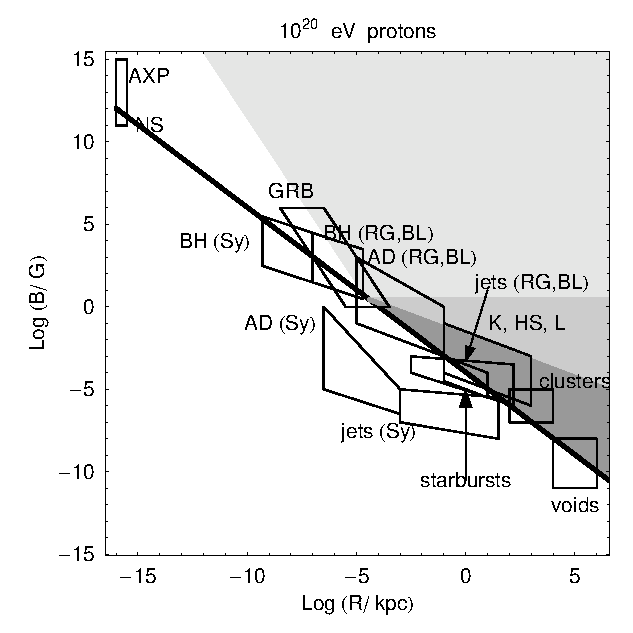
\includegraphics[width=0.5\linewidth]{figures/HillasCriterionProton20}
	\internallinenumbers
	\caption{\textbf{\textit{Hillas criterion for $\SI{1e20}\eV$ protons.}}
		This figure is reproduced here from~\cite{Ptitsyna:2008zs}.
		The black line denotes the region above which objects meet the Hillas criterion.
		The shaded regions show regions allowed for different acceleration scenarios: light gray for one-shot acceleration, gray for one-shot acceleration with synchrotron losses, and dark gray for one-shot acceleration and diffusive shock acceleration.
		Boxes denote the parameters of various astrophysical objects: the central
		parsecs (AD) of active galaxies (low-power Seyfert galaxies (Sy) and powerful radio galaxies (RG) and blazars (BL)), relativistic jets, knots (K), hot spots (HS) and lobes (L) of powerful active galaxies (RG and BL); non-relativistic jets of low-power galaxies (Sy); starburst	galaxies; gamma-ray bursts (GRB); galaxy clusters and inter-cluster voids; immediate
		the neighborhood of neutron stars (NS), anomalous X-ray pulsars and magnetars (AXP).
	}\label{fig:hillasp20}
\end{figure}

Cosmic rays can be observed interacting in the Earth's atmosphere, as they produce extensive particle air-showers whose constituents and products can be observed with a wide range of techniques.
The charged particle products of these interactions have been observed as early as 1912~\cite{hess1912uber}.
These air showers are of particular concern to neutrino detectors as they produce high-energy muons and neutrinos in relative abundance, both of which can be observed by neutrino detectors even with significant shielding and overburden.

When cosmic rays interact with the atmosphere, some nuclear fragments can be produced, but hadronization occurs due to the high energy of the incident cosmic ray and initiates a hadronic particle shower.
As part of the hadronic shower, pions and kaons are produced in abundance.
These subsequently decay or interact in the low-density atmosphere.
Leptonic and semi-leptonic decays of charged pions and kaons that produce muons or neutrinos have a large decay branching fraction, resulting in an abundance of muons and neutrinos in any air shower that begins hadronically.
Decays of charged pions
%($\pi^+\rightarrow\mu^+\nu_\mu$, $\pi^+\rightarrow\mu^+\bar{\nu}_e$, $\pi^+\rightarrow\mu^+\nu_e$, $\pi^+\rightarrow\mu^+\nu_\mu \gamma$, $\pi^+\rightarrow e^+\nu_e$),
($\pi^+\rightarrow\mu^+\nu_\mu$), 
%$K_L^0$ ($K_L^0 \rightarrow \pi^\pm e^\mp \nu_e$, $K_L^0 \rightarrow \pi^\pm \mu^\mp \nu_\mu$), and 
$K_L^0$ ($K_L^0 \rightarrow \pi^\pm e^\mp \nu_e$, $K_L^0 \rightarrow \pi^\pm \mu^\mp \nu_\mu$), and 
%$K^+$ ($K^+\rightarrow \mu^+ \nu_\mu$, $K^+\rightarrow \pi^0 e^+ \nu_e$, $K^+\rightarrow \pi^0 \mu^+ \nu_\mu$, $K^+\rightarrow \mu^+ \nu_\mu \gamma$) 
$K^+$ ($K^+\rightarrow \mu^+ \nu_\mu$, $K^+\rightarrow \pi^0 e^+ \nu_e$, $K^+\rightarrow \pi^0 \mu^+ \nu_\mu$) 
all have direct contributions to the muon and neutrino fluxes; secondary contributions from pion production in kaon decay are also present, particularly for $K_S^0$.
The yield of muons and neutrinos is highly zenith dependent.
This dependence is a result of the interplay between the probability of meson interaction and meson decay.
Unlike those that decay, pions and kaons that interact with the atmosphere or Earth will not produce neutrinos, and decay is much more likely in the low-density atmosphere.
Between the zenith and horizon, the average path length of mesons through the atmosphere increases with zenith angle, thereby increasing the yield of neutrinos for the same flux of cosmic rays.
For this reason, neutrino production from pions and kaons is peaked at the horizon, as shown in \reffig{fig:atmo_zenith}.

\begin{figure}
	\centering
	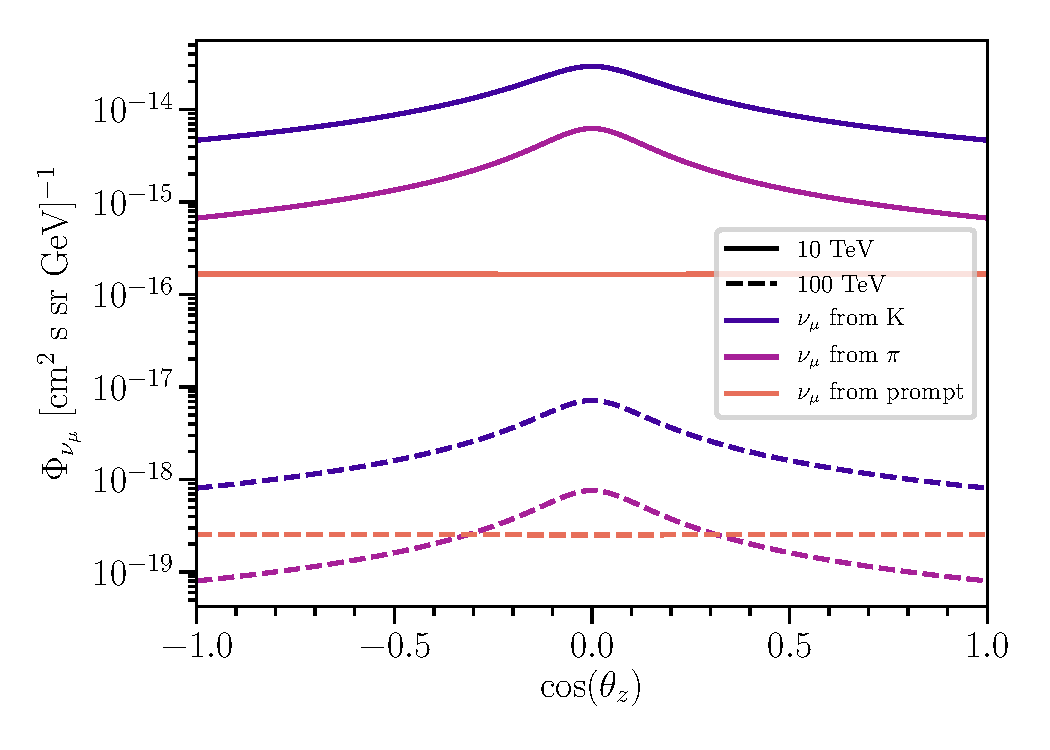
\includegraphics[width=0.7\linewidth]{figures/atm_flux}
	\internallinenumbers
	\caption{\textbf{\textit{Production of atmospheric muon neutrinos.}}
		The atmospheric muon neutrino flux at the Earth's surface is plotted as a function of the zenith angle measured with respect to the IceCube detector center.
		At these high energies above several $\si\TeV$, the production of muon neutrinos is dominated by kaon decays.
		The kaon and pion production is peaked at the horizon, where the path of these particles includes the longest stretch of atmosphere before reaching the Earth.
		This larger path length results in a higher decay probability for these mesons.
		Production from the prompt decay of charmed hadrons has no angular dependence as the decay length of these hadrons is short with respect to the atmosphere for all directions.
	}\label{fig:atmo_zenith}
\end{figure}

Neutrinos can also be produced by charmed hadrons present in air showers.
These hadrons are much shorter-lived than the pion and kaon, and almost invariably decay before interaction.
As the interaction probability for these charmed hadrons is so low, the production of neutrinos from them has practically no dependence on the zenith angle.
This flux of neutrinos is still unobserved, although its spectrum has been predicted ($\sim E^{-2.7}$) and constraints placed on its normalization.
As this atmospheric flux is effectively isotropic, some have suggested that it may be confused for the astrophysical flux.
However, the astrophysical flux can be distinguished by its energy spectrum and the effect described in \refsec{sec:passingfractions}.

Muons produced in these air showers reach the ground where they can be detected, and often penetrate many kilometers into the Earth's surface.
Underground neutrino detectors can, therefore, be sensitive to muon backgrounds despite large overburdens of rock, water, or ice.
On the other hand, Neutrinos have a small interaction cross such that the effective area for neutrinos is approximately $10^6$ times smaller than that for similar energy muons in the few $\si\TeV$ energy regime.
With this small interaction cross section, neutrinos are likely to pass through the Earth without interacting.
Neutrino detectors are then able to observe the atmospheric neutrino flux coming from all directions.
Chapter~\ref{chapter:backgrounds} explores in detail how these backgrounds are estimated for IceCube.

\begin{figure}
	\centering
	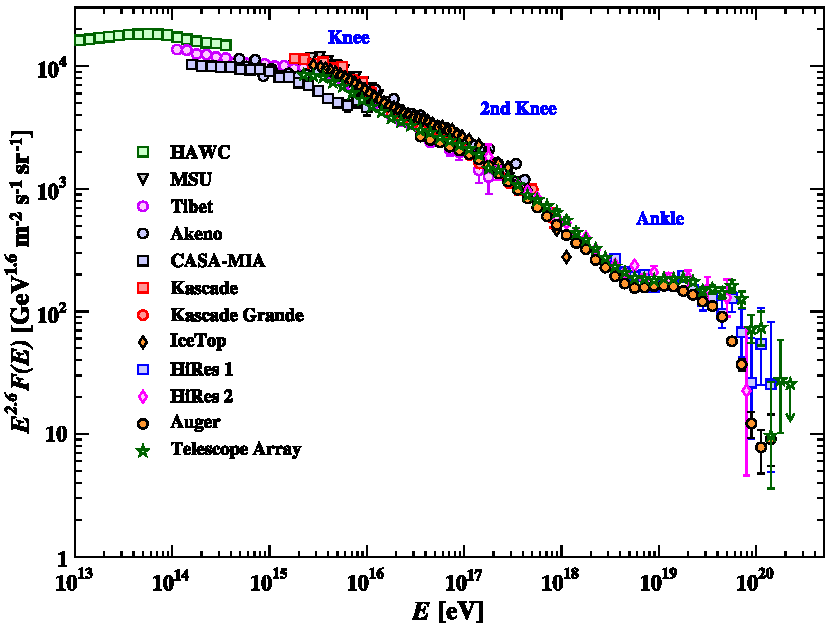
\includegraphics[width=0.8\linewidth]{figures/cosmic_ray_spectrum}
	\internallinenumbers
	\caption{\textbf{\textit{Cosmic Ray Spectrum.}}
		This figure is reproduced here from~\cite{PhysRevD.98.030001}.
		The measured flux of cosmic rays is plotted from a variety of cosmic ray observatories.
		The flux is multiplied by $E^{-2.6}$ to highlight the different spectral features.
		Above $\SI{4e18}\eV$ the harder spectrum of extra-galactic cosmic rays is apparent before the spectrum cuts off.
	}\label{fig:cosmic_ray_spectrum}
\end{figure}

\section{Neutrino interactions and detection}

Neutrinos are the only neutral leptons in the standard model of particle physics.
Although fundamentally, neutrinos only interact through gravity and the exchange of weak bosons, there exists a wide range of processes that dominate the relevant physical behavior of neutrinos at different energy scales.
Such interactions include nuclear capture, inverse beta-decay, quasi-elastic scattering, resonant particle production, coherent elastic scattering, deep inelastic scattering (DIS), and ultra-high energy interactions~\cite{Vannucci:2017rqs,Akimov:2017ade}.
Above $\si\TeV$ neutrino energies, only two known processes remain relevant for detection: DIS and resonant $W$ production.
Deep inelastic scattering refers to processes that probe the fundamental components of hadrons.
For neutrinos, this means the exchange of a weak boson with a quark.
The momentum imparted to the quark will produce a hadronic cascade of secondary particles.
The details of the lepton side of the interaction depend heavily on the species of incident neutrino and weak boson exchanged.
We can divide these DIS interactions into two categories based on the weak boson exchanged.
Interactions involving the exchange of a $Z^0$ are referred to as ``neutral current'' (NC), and those exchanging a $W^+$ or $W^-$ are referred to as ``charged current'' (CC).
Modern techniques for observing neutrino interactions rely on detecting the charged particle products of the initial interaction.
As a consequence of this, the observable energy can be very different for NC and CC events.
Both interactions produce a hadronic cascade, but on the leptonic side of the interaction, NC events have an outgoing neutrino (not observable), while CC events have an outgoing charged lepton (observable).
These two interactions are shown in \reffig{fig:DIS}.

\begin{figure}
	\centering
	\begin{tikzpicture}
	\begin{feynman}
	\vertex (a);
	\vertex [below=of a] (b);
	\vertex [above left=of a] (c) {\(\nu_{l} / \overline \nu_{l}\)};
	\vertex [above right=of a] (d) {\(\nu_{l} / \overline \nu_{l}\)};
	\vertex [below left=of b] (e) {\(u/d\)};
	\vertex [below right=of b] (f) {\(u/d\)};
	\diagram* {
		(c) -- [fermion] (a),
		(a) -- [fermion] (d),
		(e) -- [fermion] (b),
		(b) -- [fermion] (f),
		(a) -- [boson, edge label=\(Z^0\)] (b),
	};
	\end{feynman}
	\end{tikzpicture}
	\begin{tikzpicture}
	\begin{feynman}
	\vertex (a);
	\vertex [below=of a] (b);
	\vertex [above left=of a] (c) {\(\nu_{l} / \overline \nu_{l}\)};
	\vertex [above right=of a] (d) {\(l^\pm\)};
	\vertex [below left=of b] (e) {\(u/d\)};
	\vertex [below right=of b] (f) {\(d/u\)};
	\diagram* {
		(c) -- [fermion] (a),
		(a) -- [fermion] (d),
		(e) -- [fermion] (b),
		(b) -- [fermion] (f),
		(a) -- [boson, edge label=\(W^\pm\)] (b),
	};
	\end{feynman}
	\end{tikzpicture}
	\caption{The neutrino deep inelastic scattering processes NC (left) and CC (right) in matter is shown in the figure above for interactions with nucleon component quarks.
	In both cases, significant momentum can be imparted to the outgoing quark, which will result in the production of a hadronic particle cascade.
	In NC interactions, only the hadronic cascade may be detectable as the interaction product is a neutrino, which is unlikely to undergo another interaction within the detection medium.
	Interactions of the CC variety, on the other hand, produce a charged lepton in addition to the hadronic cascade.
	This charged lepton can also be detected if it receives enough energy.}
	\label{fig:DIS}
\end{figure}

The third interaction relevant above $\si\TeV$ neutrino energies is the resonant production of a $W$ boson, otherwise known as the Glashow resonance (GR)~\cite{Glashow:1960zz}.
In matter on Earth, this process occurs when an anti-electron neutrino combines with an atomic electron to produce an on-shell $W^+$ as shown in~\reffig{fig:glashow}.
If we consider the rest frame of the electron, then this resonance occurs at a neutrino energy of $\SI{6.3}\PeV$.
For atomic electrons we should consider the rest frame of the atom, and in this case there is a Doppler broadening of the resonance of $\sim\SI{20}\percent$ due to the orbital motion of the electrons~\cite{Loewy:2014zva}.
In practice, this broadening is small compared to the energy resolution of modern neutrino detectors that have access to this energy scale, and any further broadening from thermal motion will be even smaller.
The production of a $W^+$ and its subsequent decay can result in either a hadronic shower similar to a NC interaction, or a leptonic final state similar to a CC interaction.
These two possibilities correspond to the hadronic and leptonic decay modes of the $W$, respectively.

The cross section of these processes is shown as a function of the neutrino energy in \reffig{fig:nuxs}.
The growth of the cross section with energy counteracts the falling neutrino spectrum to only a small degree.
Despite the large cross section, only a few Glashow resonance events are expected in $\SI{10}\year$ of IceCube detector operation due to the comparably low neutrino flux at these energies.
Absorption of neutrinos in the Earth becomes significant above $\sim\SI{1}\TeV$, and is notably peaked near the $\SI{6.3}\PeV$ resonance energy.

\begin{figure}
	\centering
	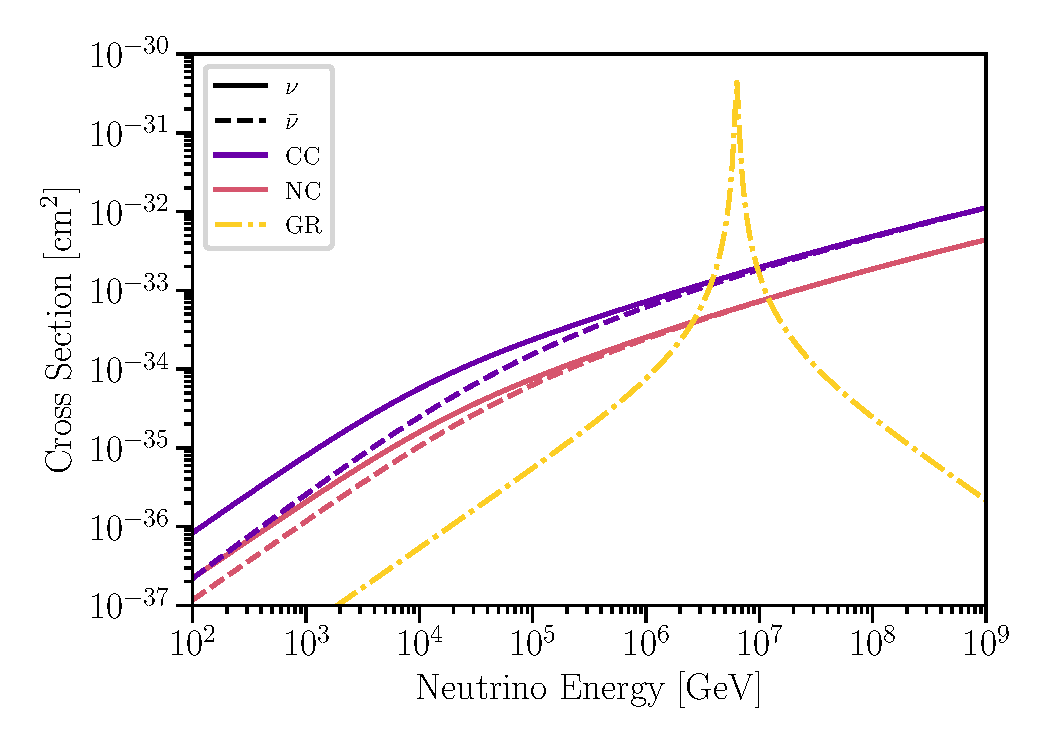
\includegraphics[width=0.8\linewidth]{figures/xs}
	\internallinenumbers
	\caption{\textbf{\textit{Neutrino interaction cross sections.}}
	Charged current (CC), neutral current (NC), and Glashow resonance (GR) cross sections are shown as a function of neutrino energy.
	The CC and NC cross sections come from~\cite{CooperSarkar:2011pa}, while the GR cross sections are computed using the forms in~\cite{Gandhi:1995tf} and corrected for the Doppler shift of electrons in the molecular orbitals of water~\cite{Loewy:2014zva}.
	}\label{fig:nuxs}
\end{figure}

\begin{figure}
	\centering
	\begin{tikzpicture}
	\begin{feynman}
	\vertex (a);
	\vertex [right=of a] (b);
	\vertex [above left=of a] (c) {\(\overline \nu_{e}\)};
	\vertex [below left=of a] (d) {\(e^-\)};
	\diagram* {
		(c) -- [fermion] (a),
		(a) -- [fermion] (d),
		(a) -- [boson, edge label=\(W^+\)] (b),
	};
	\end{feynman}
	\end{tikzpicture}
	\caption{The production of an on-shell $W^+$ boson through the combination of an anti-electron neutrino and electron.
		This resonant process occurs at neutrino energies around $\SI{6.3}\PeV$.}
	\label{fig:glashow}
\end{figure}

Through either a NC interaction or the hadronic decay of a $W$ boson, neutrinos can induce a hadronic shower.
In a hadronic shower, both charged hadrons and leptons are produced, which can be detected through well-established methods.
Charged current interactions produce a hadronic shower by imparting momentum to a quark that is then hadronized, although the charged lepton produced in the interaction is also detectable and can significantly alter the event's detection signature.

Through either a CC interaction or the leptonic decay of a $W$ boson, neutrinos can produce a detectable charged lepton, although the detection signature differs depending on the charged lepton's flavor.
Focusing on dense detection media like ice or water, the three flavors of charged leptons' detection signatures are as follows.
High energy electrons and positrons immediately interact with the detection media to initiate an electromagnetic cascade where charged leptons and high energy photons are alternately produced by one another.
This electromagnetic cascade develops over $\sim10$ radiation lengths (about $\sim\SI{5}\m$ in total) at $\SI{10}\TeV$ with a lateral extension of $\sim\SI{20}\cm$ (twice the Molière radius), expanding within the dense detection medium, and has an extreme directional bias because of the momentum of the first charged lepton.

Muons from high energy neutrino interactions do not interact as readily as electrons and positrons due to their larger mass.
Instead, muons can travel several kilometers in dense media before losing enough energy to quickly decay.
Along their entire path length, muons lose energy by interacting with the detection medium.
These ``energy loss'' interactions include ionization, electron-positron pair production, bremsstrahlung, and photo-nuclear interactions.
Although these processes are highly stochastic, the average energy loss of muons approximately follows $-dE/dx=a+bE$ where $a$ is determined by the ionization energy losses and $b$ is defined by the other processes.
In general, $a$ and $b$ are both functions of muon energy $E$, but this linear approximation where $a$ and $b$ are constant holds locally as both are slowly varying as a function of $E$.
For muon energies above $\SI{1}\TeV$, the so-called ``radiative'' term $bE$ dominates the average energy losses.
Figure~\ref{fig:energy_losses} shows the energy loss rate for the different processes.
Once the radiative losses have taken over above $\sim\SI{1}\TeV$, the losses grow exponentially with energy.

\begin{figure}
	\centering
	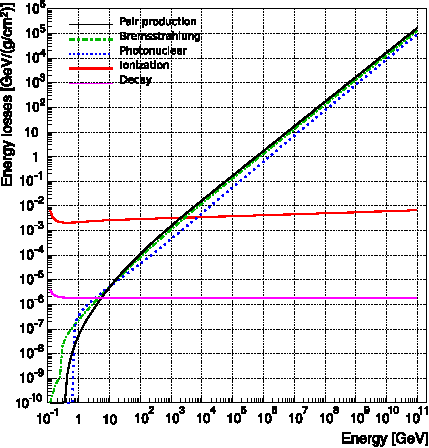
\includegraphics[width=0.8\linewidth]{figures/energy_losses}
	\internallinenumbers
	\caption{\textbf{\textit{Muon Energy Losses}}
		The muon energy loss rate computed for water is plotted as a function of the muon energy for the five different loss processes.
		This figure is reproduced here from~\cite{Koehne:2013gpa}.
		Radiative energy losses dominate above $\sim\SI{1}\TeV$.
		Although it is a smaller contribution to the energy losses, photo-nuclear interactions are the main source of uncertainty above $\sim\SI{1}\TeV$.
	}\label{fig:energy_losses}
\end{figure}

The strong dependence of the energy loss rate on muon energy means that the energy lost while traversing the detector can be used to estimate a muon's energy.
For simple observables like the total energy lost over $\SI{1}\km$ the stochastic energy losses introduce large variations between muons of the same energy, reducing their power as a proxy for the muon energy.
Figure~\ref{fig:muon_energy} shows the energy of muons lost within $\SI{1}\km$ of ice; a distribution with very long tails.
In practice the muon energy can currently be determined to within a factor of $2$, however improved techniques that take advantage of more detailed information may achieve a resolution as small as $\SI{10}\percent$ in the future.

\begin{figure}
	\centering
	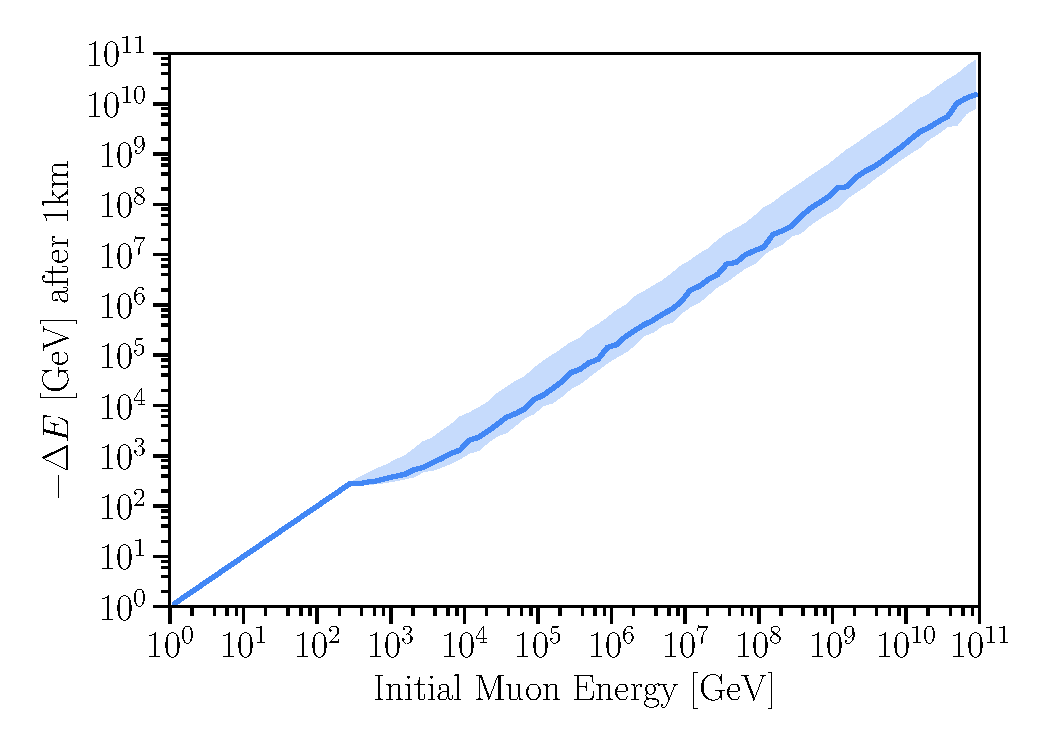
\includegraphics[width=0.8\linewidth]{figures/muon_energy}
	\internallinenumbers
	\caption{\textbf{\textit{Muon energy loss in $\SI{1}\km$ of ice.}}
		Muons are propagated through $\SI{1}\km$ of ice, and their lost energy recorded.
		For each initial muon energy, the MAP and $\SI{90}\percent$ HPD region are plotted here.
		There is a strong correlation between the initial energy and energy lost.
		However, the distribution has very long tails, making a precise determination of the muon energy based on this observable impossible.
		Below a few hundred $\si\GeV$ muons lose all of their energy within $\SI{1}\km$ of ice, narrowing the distribution of $\Delta E$.
	}\label{fig:muon_energy}
\end{figure}

Taus produced through a CC interaction, or the leptonic decay of a $W$ boson are also detectable.
The short decay length of a tau, $\SI{50}\meter / \si\PeV$, means it is likely to decay very close to the neutrino interaction vertex.
Taus decay hadronically to produce a hadronic shower with a branching ratio of $\SI{64.79}\percent$.
The tau's leptonic decay modes are decay to a charged lepton and corresponding neutrino of either electron or muon flavor.
In the electron case, an electromagnetic shower results; whereas a far traveling muon is produced in the muon case.
For taus produced via the decay of a $W$ boson, the event is indistinguishable from taus produces via CC and NC interactions other than by the resonance energy at which this process occurs.
Although a tau may traverse tens of meters, which is detectable by IceCube, the energy losses are still negligible over these distances.

From the wide variety of methods for detecting charged particles, water Cherenkov detectors are most common for detecting neutrinos in this high-energy regime above $\SI{1}\TeV$.
Water Cherenkov detectors have the advantage that their detection medium is both abundant and inexpensive, a major motivator in the design of IceCube.
Cherenkov radiation results from charged particles propagating through a dielectric medium faster than the phase velocity of light.
As charged particles pass through the dielectric material, the ionization of the medium induces the emission of light.
For particles faster than the phase velocity of emitted light, the emission forms a conical coherent wave front at a well-defined angle to the particle's path.

\begin{figure}
	\centering
	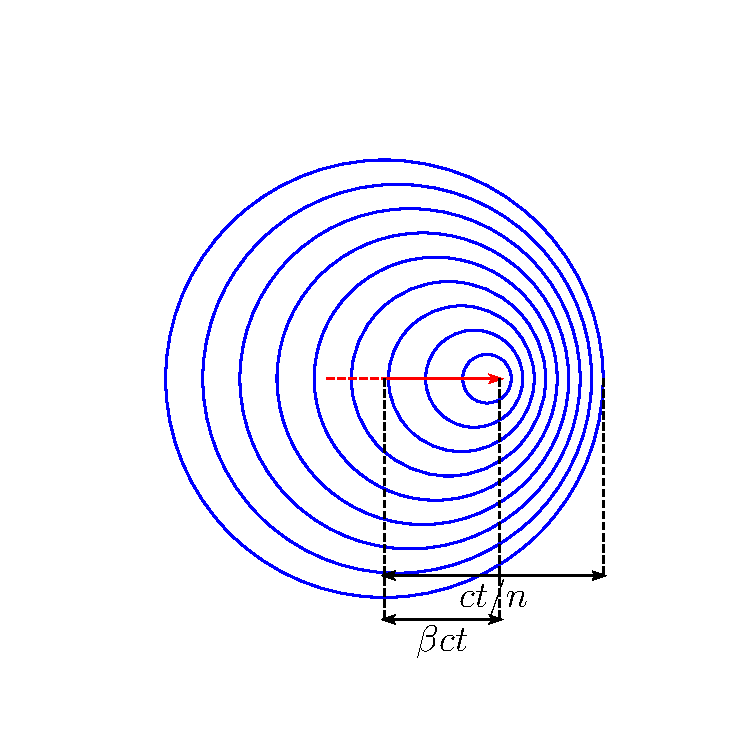
\includegraphics[width=0.45\linewidth]{figures/no_cherenkov}
	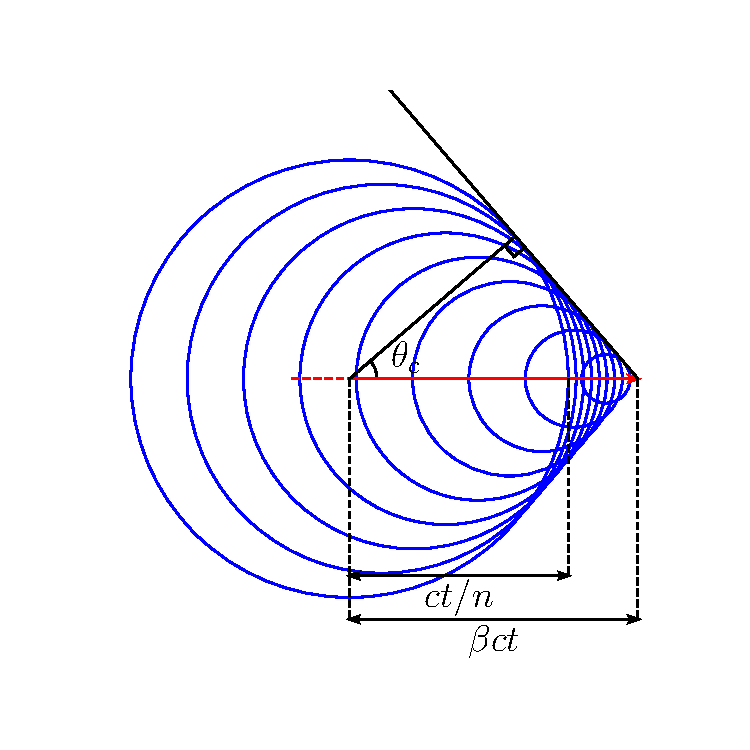
\includegraphics[width=0.45\linewidth]{figures/cherenkov}
	\internallinenumbers
	\caption{\textbf{\textit{Cherenkov radiation.}}
		This diagram shows the photon wavefronts as a charged particle moves through a dielectric medium.
		On the left for $\beta < 1/n$ and on the right for $\beta \geq 1/n$.
		The Cherenkov angle $\theta_c$ is shown on the right and describes a ray perpendicular to the coherent wavefront.
		In the Antarctic ice the Cherenkov angle $\theta_c=\SI{40.72}\degree$.
	}\label{fig:cherenkov}
\end{figure}

These detectors use Cherenkov radiation to detect particles, but the high-energy secondary charged leptons themselves contribute only a small fraction of the Cherenkov photons.
The tertiary particle showers produce most of the Cherenkov photons that these leptons give rise to when they lose energy in the detection medium.
This increased light-yield allows detectors to be sparsely instrumented while maintaining detection efficiency and reconstruction quality.

Water Cherenkov detectors often make use of photo-multiplier-tubes (PMTs) to detect Cherenkov photons.
PMTs have a thin photo-cathode held at a high-voltage differential with respect to an anode; this allows the production and acceleration of a photo-electron when photons pass through the photo-cathode.
Accelerated photo-electrons hurtle towards an amplification stage composed of many dynodes, each held at a large voltage difference to the adjacent dynodes.
This setup allows a single photo-electron to produce many secondary electrons upon interaction with a dynode, starting an exponential cascade of electrons across the dynode stages.
The resulting cascade of electrons is amplified with respect to the original signal enough to be detected electronically as a voltage change.
In this way, PMTs can be sensitive to single photons, provided one can reach the photo-cathode and produce a photo-electron.
\chapter{The IceCube Neutrino Observatory}

\section{Neutrino interactions and detection}

\section{The IceCube detector}

\begingroup
\graphicspath{{results/HESE_Final_Paper/}}
\subfile{results/HESE_Final_Paper/sections/detectorselection/detector}
\endgroup

\chapter{Statistics}\label{chapter:statistics}

\section{Systematic uncertainties and statistical treatment\label{sec:uncertainties}}
\subsection{Detector systematic uncertainties\label{sec:detector_systematics}}
\begingroup
\graphicspath{{results/HESE_Final_Paper/}}
\input{results/HESE_Final_Paper/sections/uncertainties/systematics}
\endgroup

\subsection{Statistical treatment\label{sec:statistics}}
\begingroup
\graphicspath{{results/HESE_Final_Paper/}}
\chapter{Statistics}\label{chapter:statistics}

\section{Systematic uncertainties and statistical treatment\label{sec:uncertainties}}
\subsection{Detector systematic uncertainties\label{sec:detector_systematics}}
\begingroup
\graphicspath{{results/HESE_Final_Paper/}}
\input{results/HESE_Final_Paper/sections/uncertainties/systematics}
\endgroup

\subsection{Statistical treatment\label{sec:statistics}}
\begingroup
\graphicspath{{results/HESE_Final_Paper/}}
\chapter{Statistics}\label{chapter:statistics}

\section{Systematic uncertainties and statistical treatment\label{sec:uncertainties}}
\subsection{Detector systematic uncertainties\label{sec:detector_systematics}}
\begingroup
\graphicspath{{results/HESE_Final_Paper/}}
\input{results/HESE_Final_Paper/sections/uncertainties/systematics}
\endgroup

\subsection{Statistical treatment\label{sec:statistics}}
\begingroup
\graphicspath{{results/HESE_Final_Paper/}}
\input{results/HESE_Final_Paper/sections/uncertainties/statistics}
\endgroup

\section{Dealing with limited simulation samples\label{sec:limited_simulation}}
The contents of this section is reproduced here with minor modifications from a collaborative work with Carlos A. Argüelles, and Tianlu Yuan~\cite{Arguelles:2019izp}.

\begingroup
\graphicspath{{results/mcllh_paper/}}
\input{results/mcllh_paper/sections/introduction}
\endgroup

\subsection{The Poisson likelihood and previous work\label{sec:mc_intro}}
\begingroup
\graphicspath{{results/mcllh_paper/}}
\input{results/mcllh_paper/sections/previous_work/poisson}
\endgroup

\subsubsection{The Barlow-Beeston likelihood}
\begingroup
\graphicspath{{results/mcllh_paper/}}
\input{results/mcllh_paper/sections/previous_work/bb}
\endgroup

\subsubsection{Uncertainties in the large-sample limit}
\begingroup
\graphicspath{{results/mcllh_paper/}}
\input{results/mcllh_paper/sections/previous_work/chi2}
\endgroup

\subsection{Generalization of the Poisson likelihood\label{sec:generalization_poisson}}
\begingroup
\graphicspath{{results/mcllh_paper/}}
\input{results/mcllh_paper/sections/generalized_poisson/generalized_poisson}
\endgroup

\subsubsection{Derivation of $\like (\lambda|\vecw(\vectheta))$ for identical weights\label{sec:constructing}}
\begingroup
\graphicspath{{results/mcllh_paper/}}
\input{results/mcllh_paper/sections/generalized_poisson/identical_weights}
\endgroup

\subsubsection{Extension to arbitrary weights\label{sec:extending}}
\begingroup
\graphicspath{{results/mcllh_paper/}}
\input{results/mcllh_paper/sections/generalized_poisson/arbitrary_weights}
\endgroup

\subsubsection{The effective likelihood\label{sec:effective}}
\begingroup
\graphicspath{{results/mcllh_paper/}}
\input{results/mcllh_paper/sections/generalized_poisson/effective_likelihood}
\endgroup

\subsubsection{A family of likelihoods\label{sec:priors}}
\begingroup
\graphicspath{{results/mcllh_paper/}}
\input{results/mcllh_paper/sections/generalized_poisson/family}
\endgroup

\subsubsection{Convergence of the effective likelihood\label{sec:llhconvergence}}
\begingroup
\graphicspath{{results/mcllh_paper/}}
\input{results/mcllh_paper/sections/generalized_poisson/convergence}
\endgroup

\subsubsection{Behavior of the effective likelihood\label{sec:llhbehavior}}
\begingroup
\graphicspath{{results/mcllh_paper/}}
\input{results/mcllh_paper/sections/generalized_poisson/behavior}
\endgroup

\subsection{Example and performance\label{sec:example}}
\begingroup
\graphicspath{{results/mcllh_paper/}}
\input{results/mcllh_paper/sections/example/example}
\endgroup

\subsubsection{Point estimation\label{sec:pointestimation}}
\begingroup
\graphicspath{{results/mcllh_paper/}}
\input{results/mcllh_paper/sections/example/point_estimation}
\endgroup

\subsubsection{Coverage\label{sec:coverage}}
\begingroup
\graphicspath{{results/mcllh_paper/}}
\input{results/mcllh_paper/sections/example/coverage}
\endgroup

\subsubsection{Posterior distributions\label{sec:posterior}}
\begingroup
\graphicspath{{results/mcllh_paper/}}
\input{results/mcllh_paper/sections/example/posterior}
\endgroup

\subsubsection{Performance\label{sec:performance}}
\begingroup
\graphicspath{{results/mcllh_paper/}}
\input{results/mcllh_paper/sections/example/performance}
\endgroup

\subsection{Conclusion\label{sec:llhconclusion}}
\begingroup
\graphicspath{{results/mcllh_paper/}}
\input{results/mcllh_paper/sections/conclusion}
\endgroup

\subsection{Summary of likelihood formulas\label{sec:llhtable}}
\begingroup
\graphicspath{{results/mcllh_paper/}}
\input{results/mcllh_paper/appendices/formulas}
\endgroup
\FloatBarrier
\section{Frequentist confidence intervals with nuisance parameters and limited simulation}\label{sec:low_stats_confidence_intervals}

Frequentist and Bayesian techniques deal with different two different kinds of probability.
In frequentist statistics, the relevant probability is the frequency of the outcome of a repeatable experiment.
Under this framework the important concepts are parameter estimation, confidence intervals, and statistical tests.
In Bayesian statistics, the relevant probabilities come from the application of Bayes theorem which means we can define the probability density of parameters.
This definition of the parameter p.d.f. is applicable to the same problems parameter estimation, interval construction, and statistical tests but comes at the cost of defining ``prior belief'' about parameters.

In this section we will ignore the problem of statistical tests, instead focusing on the common features that underpin parameter estimation and interval construction.
Generally in parameter estimation and interval construction there are two sets of parameters, parameters of interest $\vec\theta$ and nuisance parameters $\vec\eta$.
Fundamentally there is no distinction between these two kinds of parameters.
The difference is only in which parameters we want to infer information about.

For both parameter estimation and interval construction the likelihood function is central.
The likelihood function reflects the plausibility of model parameters given observed data and is defined as $\like(\vec\theta, \vec\eta|\textrm{data}) = p(\textrm{data}|\vec\theta, \vec\eta)$.
Where $p(\textrm{data}|\vec\theta, \vec\eta)$ is the probability of the data given the model parameters.
A useful technique to eliminate nuisance parameters is the profile likelihood technique.
Dropping the explicit notational dependence on data, the profile likelihood function is defined as
\begin{linenomath*}
	\begin{equation}
	\tilde{\like}^\texttt{profile}(\vec\theta) = \max_{\vec\eta} \like(\vec\theta,\vec\eta),
	\label{eq:likelihood_profile}
	\end{equation}
\end{linenomath*}
where often the negative log of the function is maximized in place of the function for computational reasons.
The profile likelihood is then only a function of the parameters of interest.
Parameter estimation can be performed by maximizing the profile likelihood to obtain the ``best-fit'' parameters
\begin{linenomath*}
	\begin{equation}
	\hat{\vec\theta} = \argmax_{\vec\theta} \tilde{\like}^\texttt{profile}(\vec\theta).
	\label{eq:best_fit}
	\end{equation}
\end{linenomath*}
This best-fit point in the parameter space is a derived property of the likelihood function.
However, the same procedure can be performed with other functions to the same effect.
In general a minimization procedure is used, and we refer to these functions as ``test-statistics'' (TS).
A particularly useful TS is derived directly from the profile likelihood technique,
\begin{linenomath*}
	\begin{equation}
	\TS(\vec\theta) = -2\log{\left(\frac{\tilde{\like}^\texttt{profile}(\vec\theta)}{\tilde{\like}^\texttt{profile}(\hat{\vec\theta})}\right)}.
	\end{equation}
\end{linenomath*}
Using this TS to perform parameter estimation through minimization is mathematically equivalent to maximizing the likelihood, however, this form will prove to be uniquely useful for interval construction.

Since frequentist statistics deals with the frequency of outcomes from repeated experiments we can use the TS that results from repeated experiments to construct probabilities.
Consider for a moment a single point in the parameter space $\vec\theta_0$.
At this point in the parameter space there is a distribution of data that can be observed, and therefore a distribution of TS functions.
Instead of considering the distribution of TS functions originating from this point, we can simplify the picture by looking at the TS function only evaluated at this point $\TS(\vec\theta_0)$.
This gives us a distribution of TS values for this point in the parameter space that may look like~\reffig{fig:TS_dist}.
\begin{figure}
	\centering
	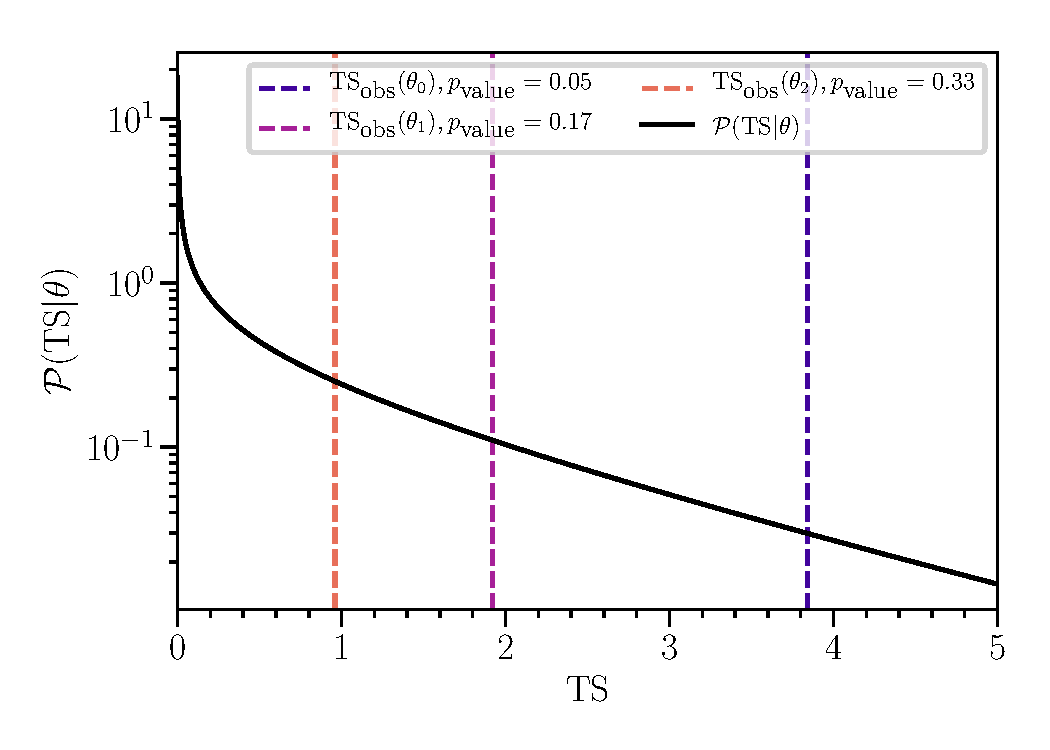
\includegraphics[width=0.8\linewidth]{figures/TS_dist}
	\caption{\textbf{\textit{Test statistic distribution.}} An example of a test statistic distribution.
	Such distributions tend to have the bulk of their mass close to the lower boundary with a long tail.
	Lower values indicate better statistical compatibility with the data.
	}
	\label{fig:TS_dist}
\end{figure}
It is important to note that for the profile likelihood TS and similar statistics a smaller TS value indicates better compatibility with the data.
For this reason many statistical tests are constructed using a single tail significance, by comparing the TS from a single experiment to a background TS distribution and reporting a p-value that is the fraction of the TS distribution greater than the observed TS.

This procedure can be extended to construct intervals by considering the TS distributions of every point in parameter space and comparing to the observed TS function.
Consider the one-dimensional case where there is a TS distribution for each value of the parameter, illustrated in~\reffig{fig:TS_dists_1d}
\begin{figure}
	\centering
	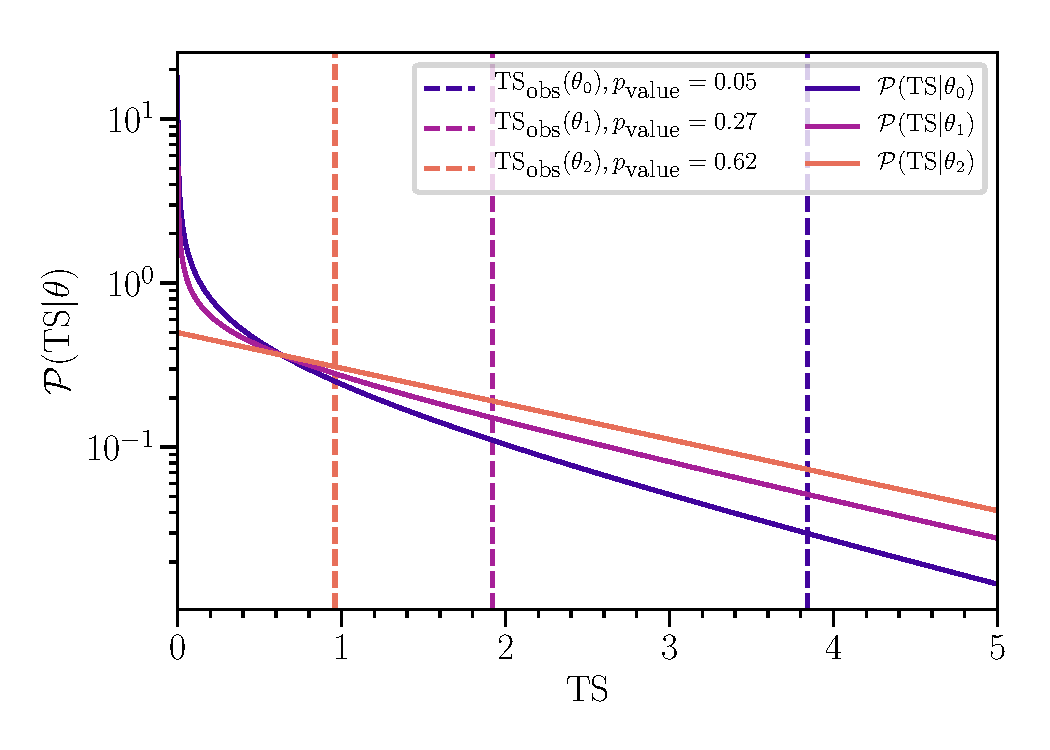
\includegraphics[width=0.8\linewidth]{figures/TS_dists_1d}
	\caption{\textbf{\textit{One-dimensional test-statistic distribution comparison.}} An example of the test statistic distributions as a function of a single parameter.
	}
	\label{fig:TS_dists_1d}
\end{figure}
We can construct an interval that will contain the true value of the parameter a fraction of the time $\alpha$ for repeated experiments.
This interval is the collection of points in the one-dimensional parameter space where the TS at that point is greater than the $\alpha$ quantile of the corresponding TS distribution.
If the TS distribution is the same for all points in parameter space, the interval construction can procedurally be thought of as drawing a horizontal line at the appropriate threshold and only including points that lie below the line.
Varying TS distributions modify this procedure to the comparison of two curves.
This procedure is not limited to one-dimension but can be extended to an arbitrary number of parameters of interest to construct n-dimensional regions with the same properties.

There is however an important caveat to this construction that appears when we consider nuisance parameters.
In order for the intervals to have the desired properties, the observed TS must be greater than the threshold for all possible values of the nuisance parameters.
This ultimatum presents several challenges.
Nuisance parameters can often have a broad or even unbounded range of allowed values, meaning if the effect of nuisance parameters does not taper off at the extrema then almost all intervals are guaranteed to be empty.
From a practical standpoint, computing the TS distributions for many points in parameter space is often done via Monte-Carlo and is computationally expensive.
Adding additional dimensions to the parameter space for which we must compute TS distributions exponentially increases the computation time.

To combat these issues we can limit our interval construction to be valid for values of the nuisance parameters that are ``reasonable''.
There are several methods for doing this, but we can split them into two categories: pure frequentist, and frequentist-Bayesian hybrid.
In the pure frequentist approaches we can either choose a single value of the nuisance parameters, or work with a limited range of the nuisance parameter values.
For the single value approach either nominal values are chosen before looking at the data, or estimators of the nuisance parameters are used to choose their values.
This approach benefits from simplicity, but fails if the test-statistic distributions vary rapidly with changes to the nuisance parameters for values that we might consider ``reasonable''.
A more expensive but robust approach is to explore the behavior of TS distributions for a limited range of the nuisance parameter values, which can be chosen {\it a priori} or from data-based bounds on the nuisance parameters.
If we are willing to consider a hybrid approach, then some more pragmatic options are available.

Although Bayesian methods could be used to choose a single point in parameter space from which to generate the TS distributions, the more interesting application is one that uses a distribution in parameter space.
In Bayesian statistics we can directly assign a probability density to the points in parameter space, either based on our prior information, or directly informed by the posterior distribution, from this extended perspective the probability of certain nuisance parameter values is of interest when considering the frequency of TS values for different parameters of interest.
The prior case is simple in that we sample the from the nuisance parameter priors when generating the TS distribution which allows us to account for variability introduced by the nuisance parameters without relying on hard cutoffs or biasing our inferences with parameter values that are unrealistic.
This prior based technique is well motivated if the priors are derived from external observations, however in the case where nuisance parameters have broad or ``uninformative'' priors this motivation and benefit may break down.
In some cases we expect nuisance parameters to be heavily constrained by the same data sample used to investigate the parameters of interest, so a different approach is merited.
The alternative is to use the posterior distribution to construct our nuisance parameter p.d.f.
Ideally a posterior distribution would be computed for each point in the parameters of interest space by fixing those parameters of interest.
In this way the nuisance parameter posterior used for sampling depends on the point in parameter space we are examining.

With the possible solutions available, we can now look at the problem of limited simulation size when generating test statistic distributions.
As explored in~\refsec{sec:limited_simulation} for binned Poisson likelihood problems, the real expectation in data or simulation for the number of events in a bin is not a known quantity.
Because the real expectations are not known, it is impossible to exactly model the distribution of TS that are expected for a particular point in the parameter space.
However, as~\refsec{sec:limited_simulation} also explored, limited simulation can be modeled with nuisance parameters so the techniques discussed above can be applied directly to the problem.
The ``single point in parameter space'' approach fails to address the additional uncertainty present in this case.
Allowing for unbounded variation of the bin expectations fails as it is guaranteed to produce empty intervals.
Bounding of the bin expectations within a reasonable range provides manageable intervals, but the dimensionality of the problem makes this computationally unfeasible beyond a handful of bins.
Unfortunately this excludes all the ``classic'' frequentist solutions to this problem.
The hybrid Bayesian-frequentist methods in this case provide a tractable solution that accounts for the additional uncertainty.
We can make use of the treatment described in~\refsec{sec:effective}, where the bin expectation is derived to be gamma distributed, and the expected number of data events modeled to be Poisson distributed once this expectation is known.
Practically this can be achieved by sampling data events from $\mcl$, or through a two step process where the expectation is sampled from a gamma distribution $\gprob(\lambda;\agpar, \bgpar)$ where $\agpar = \frac{\mu^2}{\sigma^2}+1~\textmd{and}~\bgpar=\frac{\mu}{\sigma^2}$, and the data events are sampled from a Poisson distribution $\frac{\lambda^{k}e^{-\lambda}}{k!}$.
It is important to note that this procedure only applies to variations in the data and should not be used to vary simulation expectations.
This is because the TS distribution is intended to model variations in the data, whereas the simulation used for analysis is fixed.
Combined with a similar hybrid treatment for other nuisance parameters, this provides a more complete accounting of the uncertainties given the available modeling.
\endgroup

\section{Dealing with limited simulation samples\label{sec:limited_simulation}}
The contents of this section is reproduced here with minor modifications from a collaborative work with Carlos A. Argüelles, and Tianlu Yuan~\cite{Arguelles:2019izp}.

\begingroup
\graphicspath{{results/mcllh_paper/}}
\chapter{Introduction}


\endgroup

\subsection{The Poisson likelihood and previous work\label{sec:mc_intro}}
\begingroup
\graphicspath{{results/mcllh_paper/}}
\input{results/mcllh_paper/sections/previous_work/poisson}
\endgroup

\subsubsection{The Barlow-Beeston likelihood}
\begingroup
\graphicspath{{results/mcllh_paper/}}
\input{results/mcllh_paper/sections/previous_work/bb}
\endgroup

\subsubsection{Uncertainties in the large-sample limit}
\begingroup
\graphicspath{{results/mcllh_paper/}}
\input{results/mcllh_paper/sections/previous_work/chi2}
\endgroup

\subsection{Generalization of the Poisson likelihood\label{sec:generalization_poisson}}
\begingroup
\graphicspath{{results/mcllh_paper/}}
\input{results/mcllh_paper/sections/generalized_poisson/generalized_poisson}
\endgroup

\subsubsection{Derivation of $\like (\lambda|\vecw(\vectheta))$ for identical weights\label{sec:constructing}}
\begingroup
\graphicspath{{results/mcllh_paper/}}
\input{results/mcllh_paper/sections/generalized_poisson/identical_weights}
\endgroup

\subsubsection{Extension to arbitrary weights\label{sec:extending}}
\begingroup
\graphicspath{{results/mcllh_paper/}}
\input{results/mcllh_paper/sections/generalized_poisson/arbitrary_weights}
\endgroup

\subsubsection{The effective likelihood\label{sec:effective}}
\begingroup
\graphicspath{{results/mcllh_paper/}}
\input{results/mcllh_paper/sections/generalized_poisson/effective_likelihood}
\endgroup

\subsubsection{A family of likelihoods\label{sec:priors}}
\begingroup
\graphicspath{{results/mcllh_paper/}}
\input{results/mcllh_paper/sections/generalized_poisson/family}
\endgroup

\subsubsection{Convergence of the effective likelihood\label{sec:llhconvergence}}
\begingroup
\graphicspath{{results/mcllh_paper/}}
\input{results/mcllh_paper/sections/generalized_poisson/convergence}
\endgroup

\subsubsection{Behavior of the effective likelihood\label{sec:llhbehavior}}
\begingroup
\graphicspath{{results/mcllh_paper/}}
\input{results/mcllh_paper/sections/generalized_poisson/behavior}
\endgroup

\subsection{Example and performance\label{sec:example}}
\begingroup
\graphicspath{{results/mcllh_paper/}}
\input{results/mcllh_paper/sections/example/example}
\endgroup

\subsubsection{Point estimation\label{sec:pointestimation}}
\begingroup
\graphicspath{{results/mcllh_paper/}}
\input{results/mcllh_paper/sections/example/point_estimation}
\endgroup

\subsubsection{Coverage\label{sec:coverage}}
\begingroup
\graphicspath{{results/mcllh_paper/}}
\input{results/mcllh_paper/sections/example/coverage}
\endgroup

\subsubsection{Posterior distributions\label{sec:posterior}}
\begingroup
\graphicspath{{results/mcllh_paper/}}
\input{results/mcllh_paper/sections/example/posterior}
\endgroup

\subsubsection{Performance\label{sec:performance}}
\begingroup
\graphicspath{{results/mcllh_paper/}}
\input{results/mcllh_paper/sections/example/performance}
\endgroup

\subsection{Conclusion\label{sec:llhconclusion}}
\begingroup
\graphicspath{{results/mcllh_paper/}}
\input{results/mcllh_paper/sections/conclusion}
\endgroup

\subsection{Summary of likelihood formulas\label{sec:llhtable}}
\begingroup
\graphicspath{{results/mcllh_paper/}}
\input{results/mcllh_paper/appendices/formulas}
\endgroup
\FloatBarrier
\section{Frequentist confidence intervals with nuisance parameters and limited simulation}\label{sec:low_stats_confidence_intervals}

Frequentist and Bayesian techniques deal with different two different kinds of probability.
In frequentist statistics, the relevant probability is the frequency of the outcome of a repeatable experiment.
Under this framework the important concepts are parameter estimation, confidence intervals, and statistical tests.
In Bayesian statistics, the relevant probabilities come from the application of Bayes theorem which means we can define the probability density of parameters.
This definition of the parameter p.d.f. is applicable to the same problems parameter estimation, interval construction, and statistical tests but comes at the cost of defining ``prior belief'' about parameters.

In this section we will ignore the problem of statistical tests, instead focusing on the common features that underpin parameter estimation and interval construction.
Generally in parameter estimation and interval construction there are two sets of parameters, parameters of interest $\vec\theta$ and nuisance parameters $\vec\eta$.
Fundamentally there is no distinction between these two kinds of parameters.
The difference is only in which parameters we want to infer information about.

For both parameter estimation and interval construction the likelihood function is central.
The likelihood function reflects the plausibility of model parameters given observed data and is defined as $\like(\vec\theta, \vec\eta|\textrm{data}) = p(\textrm{data}|\vec\theta, \vec\eta)$.
Where $p(\textrm{data}|\vec\theta, \vec\eta)$ is the probability of the data given the model parameters.
A useful technique to eliminate nuisance parameters is the profile likelihood technique.
Dropping the explicit notational dependence on data, the profile likelihood function is defined as
\begin{linenomath*}
	\begin{equation}
	\tilde{\like}^\texttt{profile}(\vec\theta) = \max_{\vec\eta} \like(\vec\theta,\vec\eta),
	\label{eq:likelihood_profile}
	\end{equation}
\end{linenomath*}
where often the negative log of the function is maximized in place of the function for computational reasons.
The profile likelihood is then only a function of the parameters of interest.
Parameter estimation can be performed by maximizing the profile likelihood to obtain the ``best-fit'' parameters
\begin{linenomath*}
	\begin{equation}
	\hat{\vec\theta} = \argmax_{\vec\theta} \tilde{\like}^\texttt{profile}(\vec\theta).
	\label{eq:best_fit}
	\end{equation}
\end{linenomath*}
This best-fit point in the parameter space is a derived property of the likelihood function.
However, the same procedure can be performed with other functions to the same effect.
In general a minimization procedure is used, and we refer to these functions as ``test-statistics'' (TS).
A particularly useful TS is derived directly from the profile likelihood technique,
\begin{linenomath*}
	\begin{equation}
	\TS(\vec\theta) = -2\log{\left(\frac{\tilde{\like}^\texttt{profile}(\vec\theta)}{\tilde{\like}^\texttt{profile}(\hat{\vec\theta})}\right)}.
	\end{equation}
\end{linenomath*}
Using this TS to perform parameter estimation through minimization is mathematically equivalent to maximizing the likelihood, however, this form will prove to be uniquely useful for interval construction.

Since frequentist statistics deals with the frequency of outcomes from repeated experiments we can use the TS that results from repeated experiments to construct probabilities.
Consider for a moment a single point in the parameter space $\vec\theta_0$.
At this point in the parameter space there is a distribution of data that can be observed, and therefore a distribution of TS functions.
Instead of considering the distribution of TS functions originating from this point, we can simplify the picture by looking at the TS function only evaluated at this point $\TS(\vec\theta_0)$.
This gives us a distribution of TS values for this point in the parameter space that may look like~\reffig{fig:TS_dist}.
\begin{figure}
	\centering
	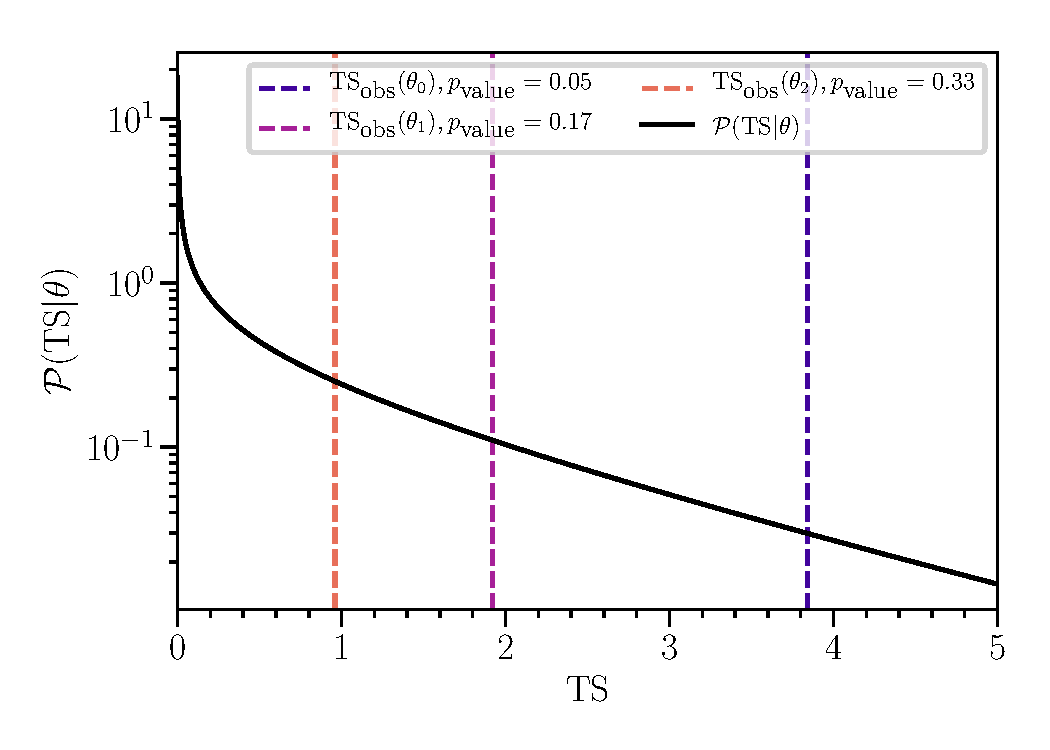
\includegraphics[width=0.8\linewidth]{figures/TS_dist}
	\caption{\textbf{\textit{Test statistic distribution.}} An example of a test statistic distribution.
	Such distributions tend to have the bulk of their mass close to the lower boundary with a long tail.
	Lower values indicate better statistical compatibility with the data.
	}
	\label{fig:TS_dist}
\end{figure}
It is important to note that for the profile likelihood TS and similar statistics a smaller TS value indicates better compatibility with the data.
For this reason many statistical tests are constructed using a single tail significance, by comparing the TS from a single experiment to a background TS distribution and reporting a p-value that is the fraction of the TS distribution greater than the observed TS.

This procedure can be extended to construct intervals by considering the TS distributions of every point in parameter space and comparing to the observed TS function.
Consider the one-dimensional case where there is a TS distribution for each value of the parameter, illustrated in~\reffig{fig:TS_dists_1d}
\begin{figure}
	\centering
	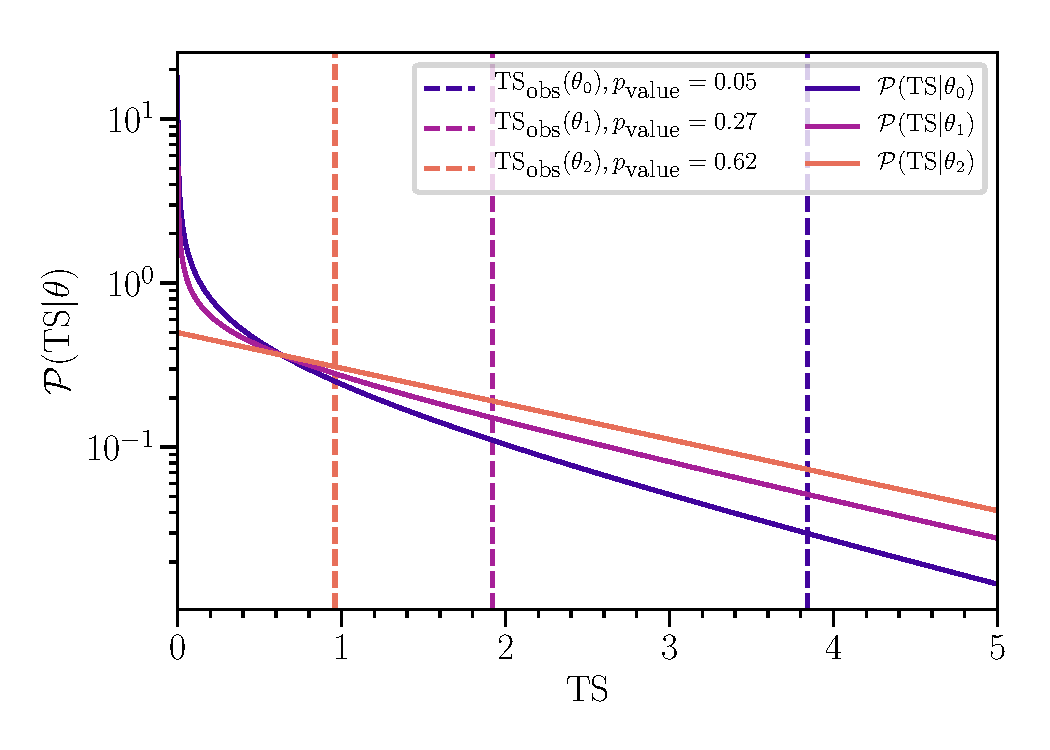
\includegraphics[width=0.8\linewidth]{figures/TS_dists_1d}
	\caption{\textbf{\textit{One-dimensional test-statistic distribution comparison.}} An example of the test statistic distributions as a function of a single parameter.
	}
	\label{fig:TS_dists_1d}
\end{figure}
We can construct an interval that will contain the true value of the parameter a fraction of the time $\alpha$ for repeated experiments.
This interval is the collection of points in the one-dimensional parameter space where the TS at that point is greater than the $\alpha$ quantile of the corresponding TS distribution.
If the TS distribution is the same for all points in parameter space, the interval construction can procedurally be thought of as drawing a horizontal line at the appropriate threshold and only including points that lie below the line.
Varying TS distributions modify this procedure to the comparison of two curves.
This procedure is not limited to one-dimension but can be extended to an arbitrary number of parameters of interest to construct n-dimensional regions with the same properties.

There is however an important caveat to this construction that appears when we consider nuisance parameters.
In order for the intervals to have the desired properties, the observed TS must be greater than the threshold for all possible values of the nuisance parameters.
This ultimatum presents several challenges.
Nuisance parameters can often have a broad or even unbounded range of allowed values, meaning if the effect of nuisance parameters does not taper off at the extrema then almost all intervals are guaranteed to be empty.
From a practical standpoint, computing the TS distributions for many points in parameter space is often done via Monte-Carlo and is computationally expensive.
Adding additional dimensions to the parameter space for which we must compute TS distributions exponentially increases the computation time.

To combat these issues we can limit our interval construction to be valid for values of the nuisance parameters that are ``reasonable''.
There are several methods for doing this, but we can split them into two categories: pure frequentist, and frequentist-Bayesian hybrid.
In the pure frequentist approaches we can either choose a single value of the nuisance parameters, or work with a limited range of the nuisance parameter values.
For the single value approach either nominal values are chosen before looking at the data, or estimators of the nuisance parameters are used to choose their values.
This approach benefits from simplicity, but fails if the test-statistic distributions vary rapidly with changes to the nuisance parameters for values that we might consider ``reasonable''.
A more expensive but robust approach is to explore the behavior of TS distributions for a limited range of the nuisance parameter values, which can be chosen {\it a priori} or from data-based bounds on the nuisance parameters.
If we are willing to consider a hybrid approach, then some more pragmatic options are available.

Although Bayesian methods could be used to choose a single point in parameter space from which to generate the TS distributions, the more interesting application is one that uses a distribution in parameter space.
In Bayesian statistics we can directly assign a probability density to the points in parameter space, either based on our prior information, or directly informed by the posterior distribution, from this extended perspective the probability of certain nuisance parameter values is of interest when considering the frequency of TS values for different parameters of interest.
The prior case is simple in that we sample the from the nuisance parameter priors when generating the TS distribution which allows us to account for variability introduced by the nuisance parameters without relying on hard cutoffs or biasing our inferences with parameter values that are unrealistic.
This prior based technique is well motivated if the priors are derived from external observations, however in the case where nuisance parameters have broad or ``uninformative'' priors this motivation and benefit may break down.
In some cases we expect nuisance parameters to be heavily constrained by the same data sample used to investigate the parameters of interest, so a different approach is merited.
The alternative is to use the posterior distribution to construct our nuisance parameter p.d.f.
Ideally a posterior distribution would be computed for each point in the parameters of interest space by fixing those parameters of interest.
In this way the nuisance parameter posterior used for sampling depends on the point in parameter space we are examining.

With the possible solutions available, we can now look at the problem of limited simulation size when generating test statistic distributions.
As explored in~\refsec{sec:limited_simulation} for binned Poisson likelihood problems, the real expectation in data or simulation for the number of events in a bin is not a known quantity.
Because the real expectations are not known, it is impossible to exactly model the distribution of TS that are expected for a particular point in the parameter space.
However, as~\refsec{sec:limited_simulation} also explored, limited simulation can be modeled with nuisance parameters so the techniques discussed above can be applied directly to the problem.
The ``single point in parameter space'' approach fails to address the additional uncertainty present in this case.
Allowing for unbounded variation of the bin expectations fails as it is guaranteed to produce empty intervals.
Bounding of the bin expectations within a reasonable range provides manageable intervals, but the dimensionality of the problem makes this computationally unfeasible beyond a handful of bins.
Unfortunately this excludes all the ``classic'' frequentist solutions to this problem.
The hybrid Bayesian-frequentist methods in this case provide a tractable solution that accounts for the additional uncertainty.
We can make use of the treatment described in~\refsec{sec:effective}, where the bin expectation is derived to be gamma distributed, and the expected number of data events modeled to be Poisson distributed once this expectation is known.
Practically this can be achieved by sampling data events from $\mcl$, or through a two step process where the expectation is sampled from a gamma distribution $\gprob(\lambda;\agpar, \bgpar)$ where $\agpar = \frac{\mu^2}{\sigma^2}+1~\textmd{and}~\bgpar=\frac{\mu}{\sigma^2}$, and the data events are sampled from a Poisson distribution $\frac{\lambda^{k}e^{-\lambda}}{k!}$.
It is important to note that this procedure only applies to variations in the data and should not be used to vary simulation expectations.
This is because the TS distribution is intended to model variations in the data, whereas the simulation used for analysis is fixed.
Combined with a similar hybrid treatment for other nuisance parameters, this provides a more complete accounting of the uncertainties given the available modeling.
\endgroup

\section{Dealing with limited simulation samples\label{sec:limited_simulation}}
The contents of this section is reproduced here with minor modifications from a collaborative work with Carlos A. Argüelles, and Tianlu Yuan~\cite{Arguelles:2019izp}.

\begingroup
\graphicspath{{results/mcllh_paper/}}
\chapter{Introduction}


\endgroup

\subsection{The Poisson likelihood and previous work\label{sec:mc_intro}}
\begingroup
\graphicspath{{results/mcllh_paper/}}
\input{results/mcllh_paper/sections/previous_work/poisson}
\endgroup

\subsubsection{The Barlow-Beeston likelihood}
\begingroup
\graphicspath{{results/mcllh_paper/}}
\input{results/mcllh_paper/sections/previous_work/bb}
\endgroup

\subsubsection{Uncertainties in the large-sample limit}
\begingroup
\graphicspath{{results/mcllh_paper/}}
\input{results/mcllh_paper/sections/previous_work/chi2}
\endgroup

\subsection{Generalization of the Poisson likelihood\label{sec:generalization_poisson}}
\begingroup
\graphicspath{{results/mcllh_paper/}}
\input{results/mcllh_paper/sections/generalized_poisson/generalized_poisson}
\endgroup

\subsubsection{Derivation of $\like (\lambda|\vecw(\vectheta))$ for identical weights\label{sec:constructing}}
\begingroup
\graphicspath{{results/mcllh_paper/}}
\input{results/mcllh_paper/sections/generalized_poisson/identical_weights}
\endgroup

\subsubsection{Extension to arbitrary weights\label{sec:extending}}
\begingroup
\graphicspath{{results/mcllh_paper/}}
\input{results/mcllh_paper/sections/generalized_poisson/arbitrary_weights}
\endgroup

\subsubsection{The effective likelihood\label{sec:effective}}
\begingroup
\graphicspath{{results/mcllh_paper/}}
\input{results/mcllh_paper/sections/generalized_poisson/effective_likelihood}
\endgroup

\subsubsection{A family of likelihoods\label{sec:priors}}
\begingroup
\graphicspath{{results/mcllh_paper/}}
\input{results/mcllh_paper/sections/generalized_poisson/family}
\endgroup

\subsubsection{Convergence of the effective likelihood\label{sec:llhconvergence}}
\begingroup
\graphicspath{{results/mcllh_paper/}}
\input{results/mcllh_paper/sections/generalized_poisson/convergence}
\endgroup

\subsubsection{Behavior of the effective likelihood\label{sec:llhbehavior}}
\begingroup
\graphicspath{{results/mcllh_paper/}}
\input{results/mcllh_paper/sections/generalized_poisson/behavior}
\endgroup

\subsection{Example and performance\label{sec:example}}
\begingroup
\graphicspath{{results/mcllh_paper/}}
\input{results/mcllh_paper/sections/example/example}
\endgroup

\subsubsection{Point estimation\label{sec:pointestimation}}
\begingroup
\graphicspath{{results/mcllh_paper/}}
\input{results/mcllh_paper/sections/example/point_estimation}
\endgroup

\subsubsection{Coverage\label{sec:coverage}}
\begingroup
\graphicspath{{results/mcllh_paper/}}
\input{results/mcllh_paper/sections/example/coverage}
\endgroup

\subsubsection{Posterior distributions\label{sec:posterior}}
\begingroup
\graphicspath{{results/mcllh_paper/}}
\input{results/mcllh_paper/sections/example/posterior}
\endgroup

\subsubsection{Performance\label{sec:performance}}
\begingroup
\graphicspath{{results/mcllh_paper/}}
\input{results/mcllh_paper/sections/example/performance}
\endgroup

\subsection{Conclusion\label{sec:llhconclusion}}
\begingroup
\graphicspath{{results/mcllh_paper/}}
\input{results/mcllh_paper/sections/conclusion}
\endgroup

\subsection{Summary of likelihood formulas\label{sec:llhtable}}
\begingroup
\graphicspath{{results/mcllh_paper/}}
\input{results/mcllh_paper/appendices/formulas}
\endgroup
\FloatBarrier
\section{Frequentist confidence intervals with nuisance parameters and limited simulation}\label{sec:low_stats_confidence_intervals}

Frequentist and Bayesian techniques deal with different two different kinds of probability.
In frequentist statistics, the relevant probability is the frequency of the outcome of a repeatable experiment.
Under this framework the important concepts are parameter estimation, confidence intervals, and statistical tests.
In Bayesian statistics, the relevant probabilities come from the application of Bayes theorem which means we can define the probability density of parameters.
This definition of the parameter p.d.f. is applicable to the same problems parameter estimation, interval construction, and statistical tests but comes at the cost of defining ``prior belief'' about parameters.

In this section we will ignore the problem of statistical tests, instead focusing on the common features that underpin parameter estimation and interval construction.
Generally in parameter estimation and interval construction there are two sets of parameters, parameters of interest $\vec\theta$ and nuisance parameters $\vec\eta$.
Fundamentally there is no distinction between these two kinds of parameters.
The difference is only in which parameters we want to infer information about.

For both parameter estimation and interval construction the likelihood function is central.
The likelihood function reflects the plausibility of model parameters given observed data and is defined as $\like(\vec\theta, \vec\eta|\textrm{data}) = p(\textrm{data}|\vec\theta, \vec\eta)$.
Where $p(\textrm{data}|\vec\theta, \vec\eta)$ is the probability of the data given the model parameters.
A useful technique to eliminate nuisance parameters is the profile likelihood technique.
Dropping the explicit notational dependence on data, the profile likelihood function is defined as
\begin{linenomath*}
	\begin{equation}
	\tilde{\like}^\texttt{profile}(\vec\theta) = \max_{\vec\eta} \like(\vec\theta,\vec\eta),
	\label{eq:likelihood_profile}
	\end{equation}
\end{linenomath*}
where often the negative log of the function is maximized in place of the function for computational reasons.
The profile likelihood is then only a function of the parameters of interest.
Parameter estimation can be performed by maximizing the profile likelihood to obtain the ``best-fit'' parameters
\begin{linenomath*}
	\begin{equation}
	\hat{\vec\theta} = \argmax_{\vec\theta} \tilde{\like}^\texttt{profile}(\vec\theta).
	\label{eq:best_fit}
	\end{equation}
\end{linenomath*}
This best-fit point in the parameter space is a derived property of the likelihood function.
However, the same procedure can be performed with other functions to the same effect.
In general a minimization procedure is used, and we refer to these functions as ``test-statistics'' (TS).
A particularly useful TS is derived directly from the profile likelihood technique,
\begin{linenomath*}
	\begin{equation}
	\TS(\vec\theta) = -2\log{\left(\frac{\tilde{\like}^\texttt{profile}(\vec\theta)}{\tilde{\like}^\texttt{profile}(\hat{\vec\theta})}\right)}.
	\end{equation}
\end{linenomath*}
Using this TS to perform parameter estimation through minimization is mathematically equivalent to maximizing the likelihood, however, this form will prove to be uniquely useful for interval construction.

Since frequentist statistics deals with the frequency of outcomes from repeated experiments we can use the TS that results from repeated experiments to construct probabilities.
Consider for a moment a single point in the parameter space $\vec\theta_0$.
At this point in the parameter space there is a distribution of data that can be observed, and therefore a distribution of TS functions.
Instead of considering the distribution of TS functions originating from this point, we can simplify the picture by looking at the TS function only evaluated at this point $\TS(\vec\theta_0)$.
This gives us a distribution of TS values for this point in the parameter space that may look like~\reffig{fig:TS_dist}.
\begin{figure}
	\centering
	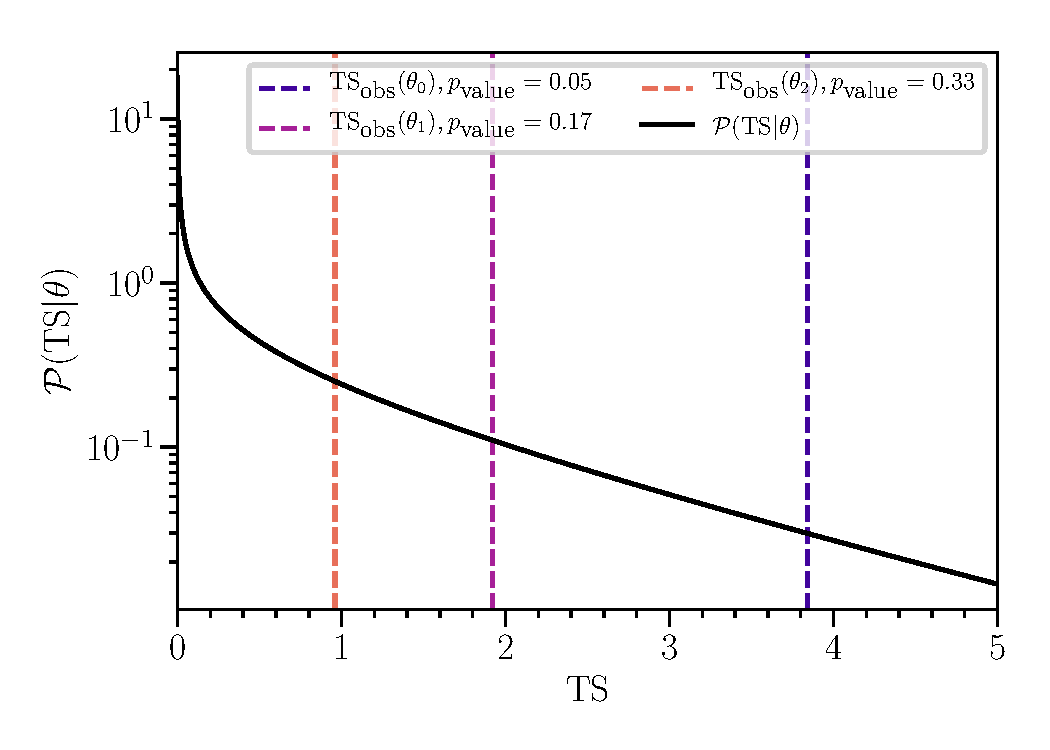
\includegraphics[width=0.8\linewidth]{figures/TS_dist}
	\caption{\textbf{\textit{Test statistic distribution.}} An example of a test statistic distribution.
	Such distributions tend to have the bulk of their mass close to the lower boundary with a long tail.
	Lower values indicate better statistical compatibility with the data.
	}
	\label{fig:TS_dist}
\end{figure}
It is important to note that for the profile likelihood TS and similar statistics a smaller TS value indicates better compatibility with the data.
For this reason many statistical tests are constructed using a single tail significance, by comparing the TS from a single experiment to a background TS distribution and reporting a p-value that is the fraction of the TS distribution greater than the observed TS.

This procedure can be extended to construct intervals by considering the TS distributions of every point in parameter space and comparing to the observed TS function.
Consider the one-dimensional case where there is a TS distribution for each value of the parameter, illustrated in~\reffig{fig:TS_dists_1d}
\begin{figure}
	\centering
	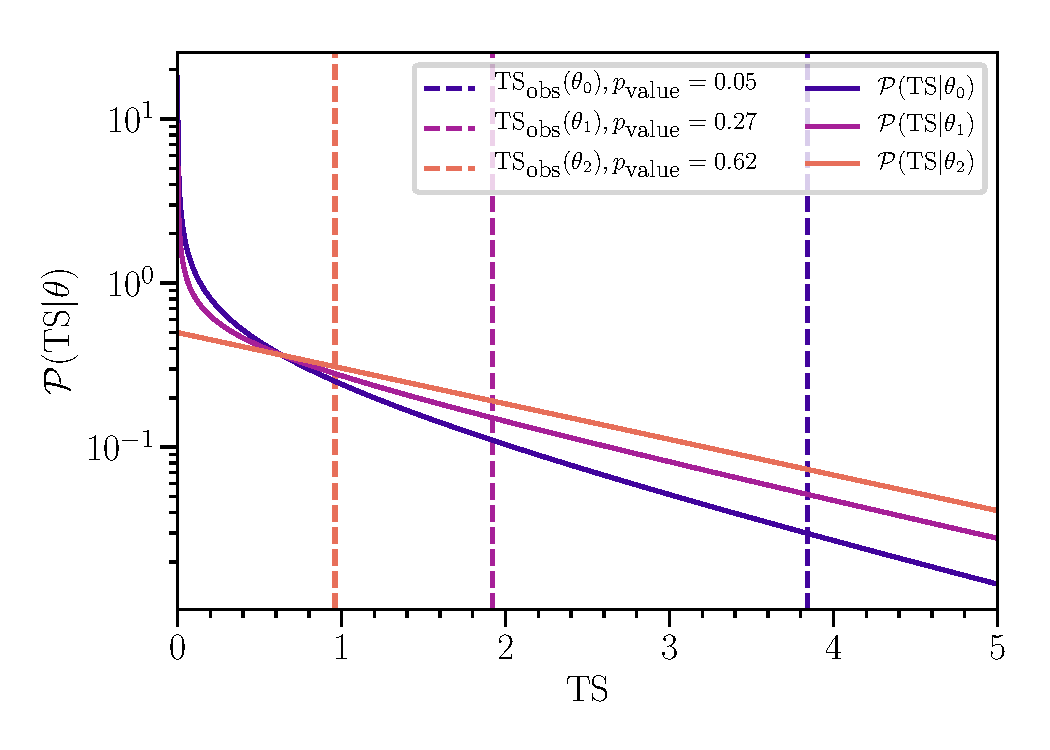
\includegraphics[width=0.8\linewidth]{figures/TS_dists_1d}
	\caption{\textbf{\textit{One-dimensional test-statistic distribution comparison.}} An example of the test statistic distributions as a function of a single parameter.
	}
	\label{fig:TS_dists_1d}
\end{figure}
We can construct an interval that will contain the true value of the parameter a fraction of the time $\alpha$ for repeated experiments.
This interval is the collection of points in the one-dimensional parameter space where the TS at that point is greater than the $\alpha$ quantile of the corresponding TS distribution.
If the TS distribution is the same for all points in parameter space, the interval construction can procedurally be thought of as drawing a horizontal line at the appropriate threshold and only including points that lie below the line.
Varying TS distributions modify this procedure to the comparison of two curves.
This procedure is not limited to one-dimension but can be extended to an arbitrary number of parameters of interest to construct n-dimensional regions with the same properties.

There is however an important caveat to this construction that appears when we consider nuisance parameters.
In order for the intervals to have the desired properties, the observed TS must be greater than the threshold for all possible values of the nuisance parameters.
This ultimatum presents several challenges.
Nuisance parameters can often have a broad or even unbounded range of allowed values, meaning if the effect of nuisance parameters does not taper off at the extrema then almost all intervals are guaranteed to be empty.
From a practical standpoint, computing the TS distributions for many points in parameter space is often done via Monte-Carlo and is computationally expensive.
Adding additional dimensions to the parameter space for which we must compute TS distributions exponentially increases the computation time.

To combat these issues we can limit our interval construction to be valid for values of the nuisance parameters that are ``reasonable''.
There are several methods for doing this, but we can split them into two categories: pure frequentist, and frequentist-Bayesian hybrid.
In the pure frequentist approaches we can either choose a single value of the nuisance parameters, or work with a limited range of the nuisance parameter values.
For the single value approach either nominal values are chosen before looking at the data, or estimators of the nuisance parameters are used to choose their values.
This approach benefits from simplicity, but fails if the test-statistic distributions vary rapidly with changes to the nuisance parameters for values that we might consider ``reasonable''.
A more expensive but robust approach is to explore the behavior of TS distributions for a limited range of the nuisance parameter values, which can be chosen {\it a priori} or from data-based bounds on the nuisance parameters.
If we are willing to consider a hybrid approach, then some more pragmatic options are available.

Although Bayesian methods could be used to choose a single point in parameter space from which to generate the TS distributions, the more interesting application is one that uses a distribution in parameter space.
In Bayesian statistics we can directly assign a probability density to the points in parameter space, either based on our prior information, or directly informed by the posterior distribution, from this extended perspective the probability of certain nuisance parameter values is of interest when considering the frequency of TS values for different parameters of interest.
The prior case is simple in that we sample the from the nuisance parameter priors when generating the TS distribution which allows us to account for variability introduced by the nuisance parameters without relying on hard cutoffs or biasing our inferences with parameter values that are unrealistic.
This prior based technique is well motivated if the priors are derived from external observations, however in the case where nuisance parameters have broad or ``uninformative'' priors this motivation and benefit may break down.
In some cases we expect nuisance parameters to be heavily constrained by the same data sample used to investigate the parameters of interest, so a different approach is merited.
The alternative is to use the posterior distribution to construct our nuisance parameter p.d.f.
Ideally a posterior distribution would be computed for each point in the parameters of interest space by fixing those parameters of interest.
In this way the nuisance parameter posterior used for sampling depends on the point in parameter space we are examining.

With the possible solutions available, we can now look at the problem of limited simulation size when generating test statistic distributions.
As explored in~\refsec{sec:limited_simulation} for binned Poisson likelihood problems, the real expectation in data or simulation for the number of events in a bin is not a known quantity.
Because the real expectations are not known, it is impossible to exactly model the distribution of TS that are expected for a particular point in the parameter space.
However, as~\refsec{sec:limited_simulation} also explored, limited simulation can be modeled with nuisance parameters so the techniques discussed above can be applied directly to the problem.
The ``single point in parameter space'' approach fails to address the additional uncertainty present in this case.
Allowing for unbounded variation of the bin expectations fails as it is guaranteed to produce empty intervals.
Bounding of the bin expectations within a reasonable range provides manageable intervals, but the dimensionality of the problem makes this computationally unfeasible beyond a handful of bins.
Unfortunately this excludes all the ``classic'' frequentist solutions to this problem.
The hybrid Bayesian-frequentist methods in this case provide a tractable solution that accounts for the additional uncertainty.
We can make use of the treatment described in~\refsec{sec:effective}, where the bin expectation is derived to be gamma distributed, and the expected number of data events modeled to be Poisson distributed once this expectation is known.
Practically this can be achieved by sampling data events from $\mcl$, or through a two step process where the expectation is sampled from a gamma distribution $\gprob(\lambda;\agpar, \bgpar)$ where $\agpar = \frac{\mu^2}{\sigma^2}+1~\textmd{and}~\bgpar=\frac{\mu}{\sigma^2}$, and the data events are sampled from a Poisson distribution $\frac{\lambda^{k}e^{-\lambda}}{k!}$.
It is important to note that this procedure only applies to variations in the data and should not be used to vary simulation expectations.
This is because the TS distribution is intended to model variations in the data, whereas the simulation used for analysis is fixed.
Combined with a similar hybrid treatment for other nuisance parameters, this provides a more complete accounting of the uncertainties given the available modeling.
\chapter{Analysis methods for small sample searches}

\chapter{Generalized framework for binned likelihood analyses}


\chapter{Searching for astrophysical neutrinos}

\section{Event selection\label{sec:selection}}
\begingroup
\graphicspath{{results/HESE_Final_Paper/}}
\chapter{Searching for astrophysical neutrinos}

\section{Event selection\label{sec:selection}}
\begingroup
\graphicspath{{results/HESE_Final_Paper/}}
\chapter{Searching for astrophysical neutrinos}

\section{Event selection\label{sec:selection}}
\begingroup
\graphicspath{{results/HESE_Final_Paper/}}
\input{results/HESE_Final_Paper/sections/detectorselection/selection}
\endgroup

\section{Reconstruction and simulation}
\begingroup
\graphicspath{{results/HESE_Final_Paper/}}
\input{results/HESE_Final_Paper/sections/reconstruction}
\endgroup

\section{Systematic uncertainties and statistical treatment\label{sec:uncertainties}}
\subsection{Detector systematic uncertainties\label{sec:detector_systematics}}
\begingroup
\graphicspath{{results/HESE_Final_Paper/}}
\input{results/HESE_Final_Paper/sections/uncertainties/systematics}
\endgroup

\subsection{Statistical treatment\label{sec:statistics}}
\begingroup
\graphicspath{{results/HESE_Final_Paper/}}
\input{results/HESE_Final_Paper/sections/uncertainties/statistics}
\endgroup

\endgroup

\section{Reconstruction and simulation}
\begingroup
\graphicspath{{results/HESE_Final_Paper/}}
\chapter{Event reconstruction and simulation}\label{chapter:reconstruction}
\begingroup
\graphicspath{{results/HESE_Final_Paper/}}
\input{results/HESE_Final_Paper/sections/reconstruction}
\endgroup
\endgroup

\section{Systematic uncertainties and statistical treatment\label{sec:uncertainties}}
\subsection{Detector systematic uncertainties\label{sec:detector_systematics}}
\begingroup
\graphicspath{{results/HESE_Final_Paper/}}
\input{results/HESE_Final_Paper/sections/uncertainties/systematics}
\endgroup

\subsection{Statistical treatment\label{sec:statistics}}
\begingroup
\graphicspath{{results/HESE_Final_Paper/}}
\chapter{Statistics}\label{chapter:statistics}

\section{Systematic uncertainties and statistical treatment\label{sec:uncertainties}}
\subsection{Detector systematic uncertainties\label{sec:detector_systematics}}
\begingroup
\graphicspath{{results/HESE_Final_Paper/}}
\input{results/HESE_Final_Paper/sections/uncertainties/systematics}
\endgroup

\subsection{Statistical treatment\label{sec:statistics}}
\begingroup
\graphicspath{{results/HESE_Final_Paper/}}
\input{results/HESE_Final_Paper/sections/uncertainties/statistics}
\endgroup

\section{Dealing with limited simulation samples\label{sec:limited_simulation}}
The contents of this section is reproduced here with minor modifications from a collaborative work with Carlos A. Argüelles, and Tianlu Yuan~\cite{Arguelles:2019izp}.

\begingroup
\graphicspath{{results/mcllh_paper/}}
\input{results/mcllh_paper/sections/introduction}
\endgroup

\subsection{The Poisson likelihood and previous work\label{sec:mc_intro}}
\begingroup
\graphicspath{{results/mcllh_paper/}}
\input{results/mcllh_paper/sections/previous_work/poisson}
\endgroup

\subsubsection{The Barlow-Beeston likelihood}
\begingroup
\graphicspath{{results/mcllh_paper/}}
\input{results/mcllh_paper/sections/previous_work/bb}
\endgroup

\subsubsection{Uncertainties in the large-sample limit}
\begingroup
\graphicspath{{results/mcllh_paper/}}
\input{results/mcllh_paper/sections/previous_work/chi2}
\endgroup

\subsection{Generalization of the Poisson likelihood\label{sec:generalization_poisson}}
\begingroup
\graphicspath{{results/mcllh_paper/}}
\input{results/mcllh_paper/sections/generalized_poisson/generalized_poisson}
\endgroup

\subsubsection{Derivation of $\like (\lambda|\vecw(\vectheta))$ for identical weights\label{sec:constructing}}
\begingroup
\graphicspath{{results/mcllh_paper/}}
\input{results/mcllh_paper/sections/generalized_poisson/identical_weights}
\endgroup

\subsubsection{Extension to arbitrary weights\label{sec:extending}}
\begingroup
\graphicspath{{results/mcllh_paper/}}
\input{results/mcllh_paper/sections/generalized_poisson/arbitrary_weights}
\endgroup

\subsubsection{The effective likelihood\label{sec:effective}}
\begingroup
\graphicspath{{results/mcllh_paper/}}
\input{results/mcllh_paper/sections/generalized_poisson/effective_likelihood}
\endgroup

\subsubsection{A family of likelihoods\label{sec:priors}}
\begingroup
\graphicspath{{results/mcllh_paper/}}
\input{results/mcllh_paper/sections/generalized_poisson/family}
\endgroup

\subsubsection{Convergence of the effective likelihood\label{sec:llhconvergence}}
\begingroup
\graphicspath{{results/mcllh_paper/}}
\input{results/mcllh_paper/sections/generalized_poisson/convergence}
\endgroup

\subsubsection{Behavior of the effective likelihood\label{sec:llhbehavior}}
\begingroup
\graphicspath{{results/mcllh_paper/}}
\input{results/mcllh_paper/sections/generalized_poisson/behavior}
\endgroup

\subsection{Example and performance\label{sec:example}}
\begingroup
\graphicspath{{results/mcllh_paper/}}
\input{results/mcllh_paper/sections/example/example}
\endgroup

\subsubsection{Point estimation\label{sec:pointestimation}}
\begingroup
\graphicspath{{results/mcllh_paper/}}
\input{results/mcllh_paper/sections/example/point_estimation}
\endgroup

\subsubsection{Coverage\label{sec:coverage}}
\begingroup
\graphicspath{{results/mcllh_paper/}}
\input{results/mcllh_paper/sections/example/coverage}
\endgroup

\subsubsection{Posterior distributions\label{sec:posterior}}
\begingroup
\graphicspath{{results/mcllh_paper/}}
\input{results/mcllh_paper/sections/example/posterior}
\endgroup

\subsubsection{Performance\label{sec:performance}}
\begingroup
\graphicspath{{results/mcllh_paper/}}
\input{results/mcllh_paper/sections/example/performance}
\endgroup

\subsection{Conclusion\label{sec:llhconclusion}}
\begingroup
\graphicspath{{results/mcllh_paper/}}
\input{results/mcllh_paper/sections/conclusion}
\endgroup

\subsection{Summary of likelihood formulas\label{sec:llhtable}}
\begingroup
\graphicspath{{results/mcllh_paper/}}
\input{results/mcllh_paper/appendices/formulas}
\endgroup
\FloatBarrier
\section{Frequentist confidence intervals with nuisance parameters and limited simulation}\label{sec:low_stats_confidence_intervals}

Frequentist and Bayesian techniques deal with different two different kinds of probability.
In frequentist statistics, the relevant probability is the frequency of the outcome of a repeatable experiment.
Under this framework the important concepts are parameter estimation, confidence intervals, and statistical tests.
In Bayesian statistics, the relevant probabilities come from the application of Bayes theorem which means we can define the probability density of parameters.
This definition of the parameter p.d.f. is applicable to the same problems parameter estimation, interval construction, and statistical tests but comes at the cost of defining ``prior belief'' about parameters.

In this section we will ignore the problem of statistical tests, instead focusing on the common features that underpin parameter estimation and interval construction.
Generally in parameter estimation and interval construction there are two sets of parameters, parameters of interest $\vec\theta$ and nuisance parameters $\vec\eta$.
Fundamentally there is no distinction between these two kinds of parameters.
The difference is only in which parameters we want to infer information about.

For both parameter estimation and interval construction the likelihood function is central.
The likelihood function reflects the plausibility of model parameters given observed data and is defined as $\like(\vec\theta, \vec\eta|\textrm{data}) = p(\textrm{data}|\vec\theta, \vec\eta)$.
Where $p(\textrm{data}|\vec\theta, \vec\eta)$ is the probability of the data given the model parameters.
A useful technique to eliminate nuisance parameters is the profile likelihood technique.
Dropping the explicit notational dependence on data, the profile likelihood function is defined as
\begin{linenomath*}
	\begin{equation}
	\tilde{\like}^\texttt{profile}(\vec\theta) = \max_{\vec\eta} \like(\vec\theta,\vec\eta),
	\label{eq:likelihood_profile}
	\end{equation}
\end{linenomath*}
where often the negative log of the function is maximized in place of the function for computational reasons.
The profile likelihood is then only a function of the parameters of interest.
Parameter estimation can be performed by maximizing the profile likelihood to obtain the ``best-fit'' parameters
\begin{linenomath*}
	\begin{equation}
	\hat{\vec\theta} = \argmax_{\vec\theta} \tilde{\like}^\texttt{profile}(\vec\theta).
	\label{eq:best_fit}
	\end{equation}
\end{linenomath*}
This best-fit point in the parameter space is a derived property of the likelihood function.
However, the same procedure can be performed with other functions to the same effect.
In general a minimization procedure is used, and we refer to these functions as ``test-statistics'' (TS).
A particularly useful TS is derived directly from the profile likelihood technique,
\begin{linenomath*}
	\begin{equation}
	\TS(\vec\theta) = -2\log{\left(\frac{\tilde{\like}^\texttt{profile}(\vec\theta)}{\tilde{\like}^\texttt{profile}(\hat{\vec\theta})}\right)}.
	\end{equation}
\end{linenomath*}
Using this TS to perform parameter estimation through minimization is mathematically equivalent to maximizing the likelihood, however, this form will prove to be uniquely useful for interval construction.

Since frequentist statistics deals with the frequency of outcomes from repeated experiments we can use the TS that results from repeated experiments to construct probabilities.
Consider for a moment a single point in the parameter space $\vec\theta_0$.
At this point in the parameter space there is a distribution of data that can be observed, and therefore a distribution of TS functions.
Instead of considering the distribution of TS functions originating from this point, we can simplify the picture by looking at the TS function only evaluated at this point $\TS(\vec\theta_0)$.
This gives us a distribution of TS values for this point in the parameter space that may look like~\reffig{fig:TS_dist}.
\begin{figure}
	\centering
	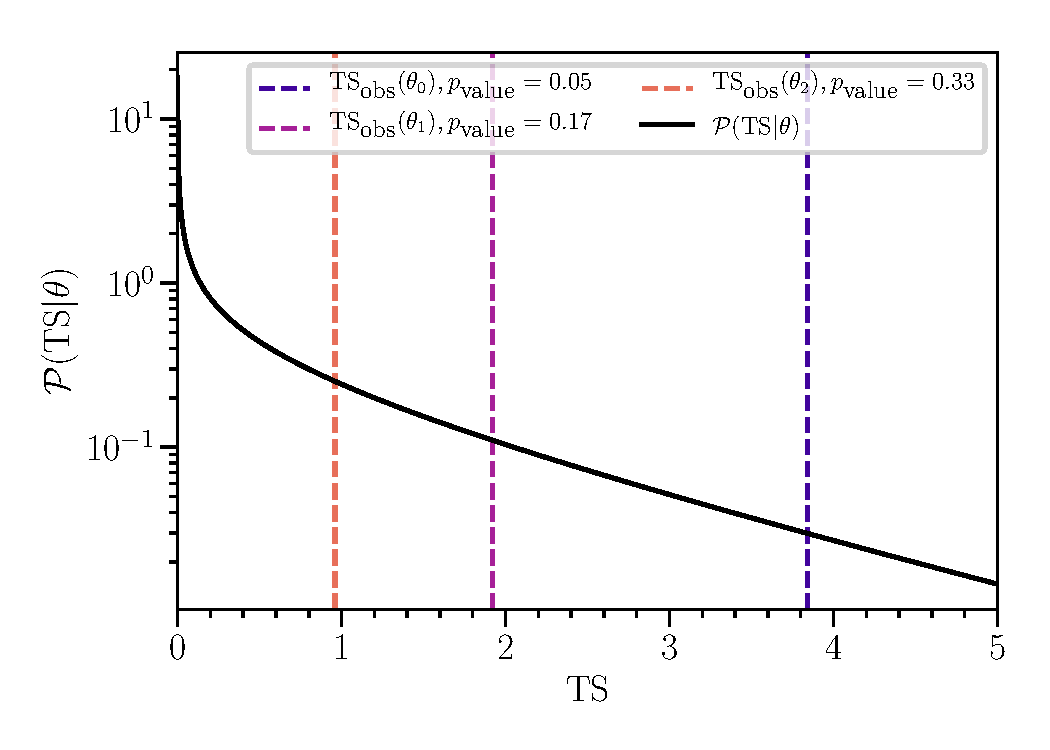
\includegraphics[width=0.8\linewidth]{figures/TS_dist}
	\caption{\textbf{\textit{Test statistic distribution.}} An example of a test statistic distribution.
	Such distributions tend to have the bulk of their mass close to the lower boundary with a long tail.
	Lower values indicate better statistical compatibility with the data.
	}
	\label{fig:TS_dist}
\end{figure}
It is important to note that for the profile likelihood TS and similar statistics a smaller TS value indicates better compatibility with the data.
For this reason many statistical tests are constructed using a single tail significance, by comparing the TS from a single experiment to a background TS distribution and reporting a p-value that is the fraction of the TS distribution greater than the observed TS.

This procedure can be extended to construct intervals by considering the TS distributions of every point in parameter space and comparing to the observed TS function.
Consider the one-dimensional case where there is a TS distribution for each value of the parameter, illustrated in~\reffig{fig:TS_dists_1d}
\begin{figure}
	\centering
	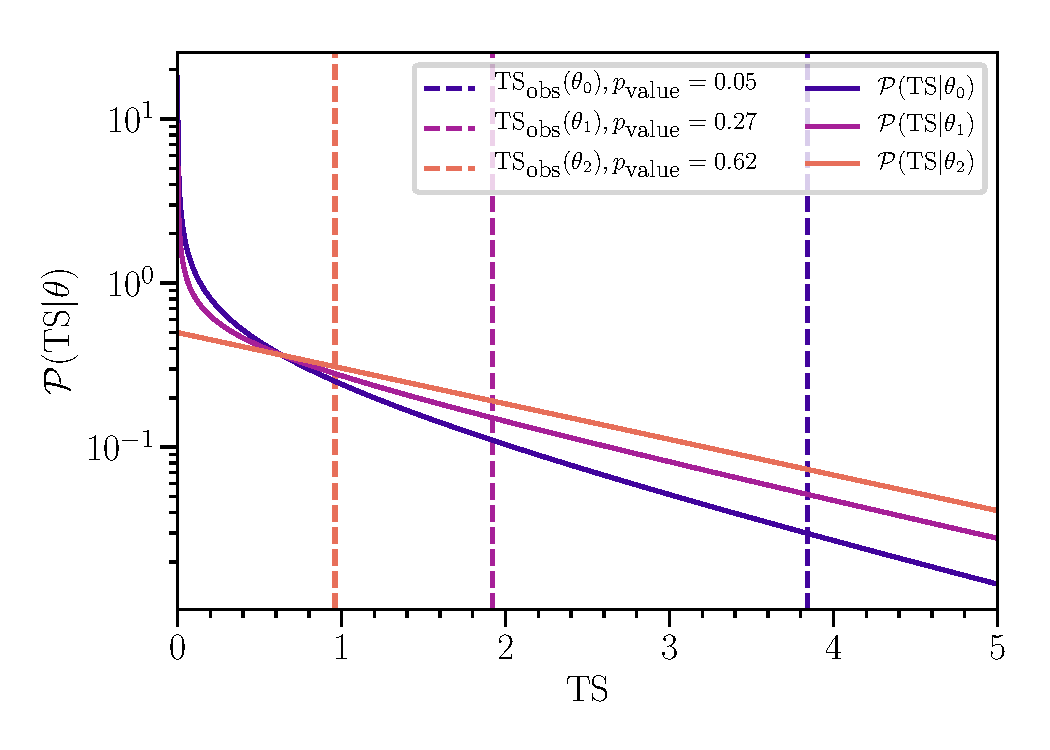
\includegraphics[width=0.8\linewidth]{figures/TS_dists_1d}
	\caption{\textbf{\textit{One-dimensional test-statistic distribution comparison.}} An example of the test statistic distributions as a function of a single parameter.
	}
	\label{fig:TS_dists_1d}
\end{figure}
We can construct an interval that will contain the true value of the parameter a fraction of the time $\alpha$ for repeated experiments.
This interval is the collection of points in the one-dimensional parameter space where the TS at that point is greater than the $\alpha$ quantile of the corresponding TS distribution.
If the TS distribution is the same for all points in parameter space, the interval construction can procedurally be thought of as drawing a horizontal line at the appropriate threshold and only including points that lie below the line.
Varying TS distributions modify this procedure to the comparison of two curves.
This procedure is not limited to one-dimension but can be extended to an arbitrary number of parameters of interest to construct n-dimensional regions with the same properties.

There is however an important caveat to this construction that appears when we consider nuisance parameters.
In order for the intervals to have the desired properties, the observed TS must be greater than the threshold for all possible values of the nuisance parameters.
This ultimatum presents several challenges.
Nuisance parameters can often have a broad or even unbounded range of allowed values, meaning if the effect of nuisance parameters does not taper off at the extrema then almost all intervals are guaranteed to be empty.
From a practical standpoint, computing the TS distributions for many points in parameter space is often done via Monte-Carlo and is computationally expensive.
Adding additional dimensions to the parameter space for which we must compute TS distributions exponentially increases the computation time.

To combat these issues we can limit our interval construction to be valid for values of the nuisance parameters that are ``reasonable''.
There are several methods for doing this, but we can split them into two categories: pure frequentist, and frequentist-Bayesian hybrid.
In the pure frequentist approaches we can either choose a single value of the nuisance parameters, or work with a limited range of the nuisance parameter values.
For the single value approach either nominal values are chosen before looking at the data, or estimators of the nuisance parameters are used to choose their values.
This approach benefits from simplicity, but fails if the test-statistic distributions vary rapidly with changes to the nuisance parameters for values that we might consider ``reasonable''.
A more expensive but robust approach is to explore the behavior of TS distributions for a limited range of the nuisance parameter values, which can be chosen {\it a priori} or from data-based bounds on the nuisance parameters.
If we are willing to consider a hybrid approach, then some more pragmatic options are available.

Although Bayesian methods could be used to choose a single point in parameter space from which to generate the TS distributions, the more interesting application is one that uses a distribution in parameter space.
In Bayesian statistics we can directly assign a probability density to the points in parameter space, either based on our prior information, or directly informed by the posterior distribution, from this extended perspective the probability of certain nuisance parameter values is of interest when considering the frequency of TS values for different parameters of interest.
The prior case is simple in that we sample the from the nuisance parameter priors when generating the TS distribution which allows us to account for variability introduced by the nuisance parameters without relying on hard cutoffs or biasing our inferences with parameter values that are unrealistic.
This prior based technique is well motivated if the priors are derived from external observations, however in the case where nuisance parameters have broad or ``uninformative'' priors this motivation and benefit may break down.
In some cases we expect nuisance parameters to be heavily constrained by the same data sample used to investigate the parameters of interest, so a different approach is merited.
The alternative is to use the posterior distribution to construct our nuisance parameter p.d.f.
Ideally a posterior distribution would be computed for each point in the parameters of interest space by fixing those parameters of interest.
In this way the nuisance parameter posterior used for sampling depends on the point in parameter space we are examining.

With the possible solutions available, we can now look at the problem of limited simulation size when generating test statistic distributions.
As explored in~\refsec{sec:limited_simulation} for binned Poisson likelihood problems, the real expectation in data or simulation for the number of events in a bin is not a known quantity.
Because the real expectations are not known, it is impossible to exactly model the distribution of TS that are expected for a particular point in the parameter space.
However, as~\refsec{sec:limited_simulation} also explored, limited simulation can be modeled with nuisance parameters so the techniques discussed above can be applied directly to the problem.
The ``single point in parameter space'' approach fails to address the additional uncertainty present in this case.
Allowing for unbounded variation of the bin expectations fails as it is guaranteed to produce empty intervals.
Bounding of the bin expectations within a reasonable range provides manageable intervals, but the dimensionality of the problem makes this computationally unfeasible beyond a handful of bins.
Unfortunately this excludes all the ``classic'' frequentist solutions to this problem.
The hybrid Bayesian-frequentist methods in this case provide a tractable solution that accounts for the additional uncertainty.
We can make use of the treatment described in~\refsec{sec:effective}, where the bin expectation is derived to be gamma distributed, and the expected number of data events modeled to be Poisson distributed once this expectation is known.
Practically this can be achieved by sampling data events from $\mcl$, or through a two step process where the expectation is sampled from a gamma distribution $\gprob(\lambda;\agpar, \bgpar)$ where $\agpar = \frac{\mu^2}{\sigma^2}+1~\textmd{and}~\bgpar=\frac{\mu}{\sigma^2}$, and the data events are sampled from a Poisson distribution $\frac{\lambda^{k}e^{-\lambda}}{k!}$.
It is important to note that this procedure only applies to variations in the data and should not be used to vary simulation expectations.
This is because the TS distribution is intended to model variations in the data, whereas the simulation used for analysis is fixed.
Combined with a similar hybrid treatment for other nuisance parameters, this provides a more complete accounting of the uncertainties given the available modeling.
\endgroup

\endgroup

\section{Reconstruction and simulation}
\begingroup
\graphicspath{{results/HESE_Final_Paper/}}
\chapter{Event reconstruction and simulation}\label{chapter:reconstruction}
\begingroup
\graphicspath{{results/HESE_Final_Paper/}}
\chapter{Event reconstruction and simulation}\label{chapter:reconstruction}
\begingroup
\graphicspath{{results/HESE_Final_Paper/}}
\input{results/HESE_Final_Paper/sections/reconstruction}
\endgroup
\endgroup
\endgroup

\section{Systematic uncertainties and statistical treatment\label{sec:uncertainties}}
\subsection{Detector systematic uncertainties\label{sec:detector_systematics}}
\begingroup
\graphicspath{{results/HESE_Final_Paper/}}
\input{results/HESE_Final_Paper/sections/uncertainties/systematics}
\endgroup

\subsection{Statistical treatment\label{sec:statistics}}
\begingroup
\graphicspath{{results/HESE_Final_Paper/}}
\chapter{Statistics}\label{chapter:statistics}

\section{Systematic uncertainties and statistical treatment\label{sec:uncertainties}}
\subsection{Detector systematic uncertainties\label{sec:detector_systematics}}
\begingroup
\graphicspath{{results/HESE_Final_Paper/}}
\input{results/HESE_Final_Paper/sections/uncertainties/systematics}
\endgroup

\subsection{Statistical treatment\label{sec:statistics}}
\begingroup
\graphicspath{{results/HESE_Final_Paper/}}
\chapter{Statistics}\label{chapter:statistics}

\section{Systematic uncertainties and statistical treatment\label{sec:uncertainties}}
\subsection{Detector systematic uncertainties\label{sec:detector_systematics}}
\begingroup
\graphicspath{{results/HESE_Final_Paper/}}
\input{results/HESE_Final_Paper/sections/uncertainties/systematics}
\endgroup

\subsection{Statistical treatment\label{sec:statistics}}
\begingroup
\graphicspath{{results/HESE_Final_Paper/}}
\input{results/HESE_Final_Paper/sections/uncertainties/statistics}
\endgroup

\section{Dealing with limited simulation samples\label{sec:limited_simulation}}
The contents of this section is reproduced here with minor modifications from a collaborative work with Carlos A. Argüelles, and Tianlu Yuan~\cite{Arguelles:2019izp}.

\begingroup
\graphicspath{{results/mcllh_paper/}}
\input{results/mcllh_paper/sections/introduction}
\endgroup

\subsection{The Poisson likelihood and previous work\label{sec:mc_intro}}
\begingroup
\graphicspath{{results/mcllh_paper/}}
\input{results/mcllh_paper/sections/previous_work/poisson}
\endgroup

\subsubsection{The Barlow-Beeston likelihood}
\begingroup
\graphicspath{{results/mcllh_paper/}}
\input{results/mcllh_paper/sections/previous_work/bb}
\endgroup

\subsubsection{Uncertainties in the large-sample limit}
\begingroup
\graphicspath{{results/mcllh_paper/}}
\input{results/mcllh_paper/sections/previous_work/chi2}
\endgroup

\subsection{Generalization of the Poisson likelihood\label{sec:generalization_poisson}}
\begingroup
\graphicspath{{results/mcllh_paper/}}
\input{results/mcllh_paper/sections/generalized_poisson/generalized_poisson}
\endgroup

\subsubsection{Derivation of $\like (\lambda|\vecw(\vectheta))$ for identical weights\label{sec:constructing}}
\begingroup
\graphicspath{{results/mcllh_paper/}}
\input{results/mcllh_paper/sections/generalized_poisson/identical_weights}
\endgroup

\subsubsection{Extension to arbitrary weights\label{sec:extending}}
\begingroup
\graphicspath{{results/mcllh_paper/}}
\input{results/mcllh_paper/sections/generalized_poisson/arbitrary_weights}
\endgroup

\subsubsection{The effective likelihood\label{sec:effective}}
\begingroup
\graphicspath{{results/mcllh_paper/}}
\input{results/mcllh_paper/sections/generalized_poisson/effective_likelihood}
\endgroup

\subsubsection{A family of likelihoods\label{sec:priors}}
\begingroup
\graphicspath{{results/mcllh_paper/}}
\input{results/mcllh_paper/sections/generalized_poisson/family}
\endgroup

\subsubsection{Convergence of the effective likelihood\label{sec:llhconvergence}}
\begingroup
\graphicspath{{results/mcllh_paper/}}
\input{results/mcllh_paper/sections/generalized_poisson/convergence}
\endgroup

\subsubsection{Behavior of the effective likelihood\label{sec:llhbehavior}}
\begingroup
\graphicspath{{results/mcllh_paper/}}
\input{results/mcllh_paper/sections/generalized_poisson/behavior}
\endgroup

\subsection{Example and performance\label{sec:example}}
\begingroup
\graphicspath{{results/mcllh_paper/}}
\input{results/mcllh_paper/sections/example/example}
\endgroup

\subsubsection{Point estimation\label{sec:pointestimation}}
\begingroup
\graphicspath{{results/mcllh_paper/}}
\input{results/mcllh_paper/sections/example/point_estimation}
\endgroup

\subsubsection{Coverage\label{sec:coverage}}
\begingroup
\graphicspath{{results/mcllh_paper/}}
\input{results/mcllh_paper/sections/example/coverage}
\endgroup

\subsubsection{Posterior distributions\label{sec:posterior}}
\begingroup
\graphicspath{{results/mcllh_paper/}}
\input{results/mcllh_paper/sections/example/posterior}
\endgroup

\subsubsection{Performance\label{sec:performance}}
\begingroup
\graphicspath{{results/mcllh_paper/}}
\input{results/mcllh_paper/sections/example/performance}
\endgroup

\subsection{Conclusion\label{sec:llhconclusion}}
\begingroup
\graphicspath{{results/mcllh_paper/}}
\input{results/mcllh_paper/sections/conclusion}
\endgroup

\subsection{Summary of likelihood formulas\label{sec:llhtable}}
\begingroup
\graphicspath{{results/mcllh_paper/}}
\input{results/mcllh_paper/appendices/formulas}
\endgroup
\FloatBarrier
\section{Frequentist confidence intervals with nuisance parameters and limited simulation}\label{sec:low_stats_confidence_intervals}

Frequentist and Bayesian techniques deal with different two different kinds of probability.
In frequentist statistics, the relevant probability is the frequency of the outcome of a repeatable experiment.
Under this framework the important concepts are parameter estimation, confidence intervals, and statistical tests.
In Bayesian statistics, the relevant probabilities come from the application of Bayes theorem which means we can define the probability density of parameters.
This definition of the parameter p.d.f. is applicable to the same problems parameter estimation, interval construction, and statistical tests but comes at the cost of defining ``prior belief'' about parameters.

In this section we will ignore the problem of statistical tests, instead focusing on the common features that underpin parameter estimation and interval construction.
Generally in parameter estimation and interval construction there are two sets of parameters, parameters of interest $\vec\theta$ and nuisance parameters $\vec\eta$.
Fundamentally there is no distinction between these two kinds of parameters.
The difference is only in which parameters we want to infer information about.

For both parameter estimation and interval construction the likelihood function is central.
The likelihood function reflects the plausibility of model parameters given observed data and is defined as $\like(\vec\theta, \vec\eta|\textrm{data}) = p(\textrm{data}|\vec\theta, \vec\eta)$.
Where $p(\textrm{data}|\vec\theta, \vec\eta)$ is the probability of the data given the model parameters.
A useful technique to eliminate nuisance parameters is the profile likelihood technique.
Dropping the explicit notational dependence on data, the profile likelihood function is defined as
\begin{linenomath*}
	\begin{equation}
	\tilde{\like}^\texttt{profile}(\vec\theta) = \max_{\vec\eta} \like(\vec\theta,\vec\eta),
	\label{eq:likelihood_profile}
	\end{equation}
\end{linenomath*}
where often the negative log of the function is maximized in place of the function for computational reasons.
The profile likelihood is then only a function of the parameters of interest.
Parameter estimation can be performed by maximizing the profile likelihood to obtain the ``best-fit'' parameters
\begin{linenomath*}
	\begin{equation}
	\hat{\vec\theta} = \argmax_{\vec\theta} \tilde{\like}^\texttt{profile}(\vec\theta).
	\label{eq:best_fit}
	\end{equation}
\end{linenomath*}
This best-fit point in the parameter space is a derived property of the likelihood function.
However, the same procedure can be performed with other functions to the same effect.
In general a minimization procedure is used, and we refer to these functions as ``test-statistics'' (TS).
A particularly useful TS is derived directly from the profile likelihood technique,
\begin{linenomath*}
	\begin{equation}
	\TS(\vec\theta) = -2\log{\left(\frac{\tilde{\like}^\texttt{profile}(\vec\theta)}{\tilde{\like}^\texttt{profile}(\hat{\vec\theta})}\right)}.
	\end{equation}
\end{linenomath*}
Using this TS to perform parameter estimation through minimization is mathematically equivalent to maximizing the likelihood, however, this form will prove to be uniquely useful for interval construction.

Since frequentist statistics deals with the frequency of outcomes from repeated experiments we can use the TS that results from repeated experiments to construct probabilities.
Consider for a moment a single point in the parameter space $\vec\theta_0$.
At this point in the parameter space there is a distribution of data that can be observed, and therefore a distribution of TS functions.
Instead of considering the distribution of TS functions originating from this point, we can simplify the picture by looking at the TS function only evaluated at this point $\TS(\vec\theta_0)$.
This gives us a distribution of TS values for this point in the parameter space that may look like~\reffig{fig:TS_dist}.
\begin{figure}
	\centering
	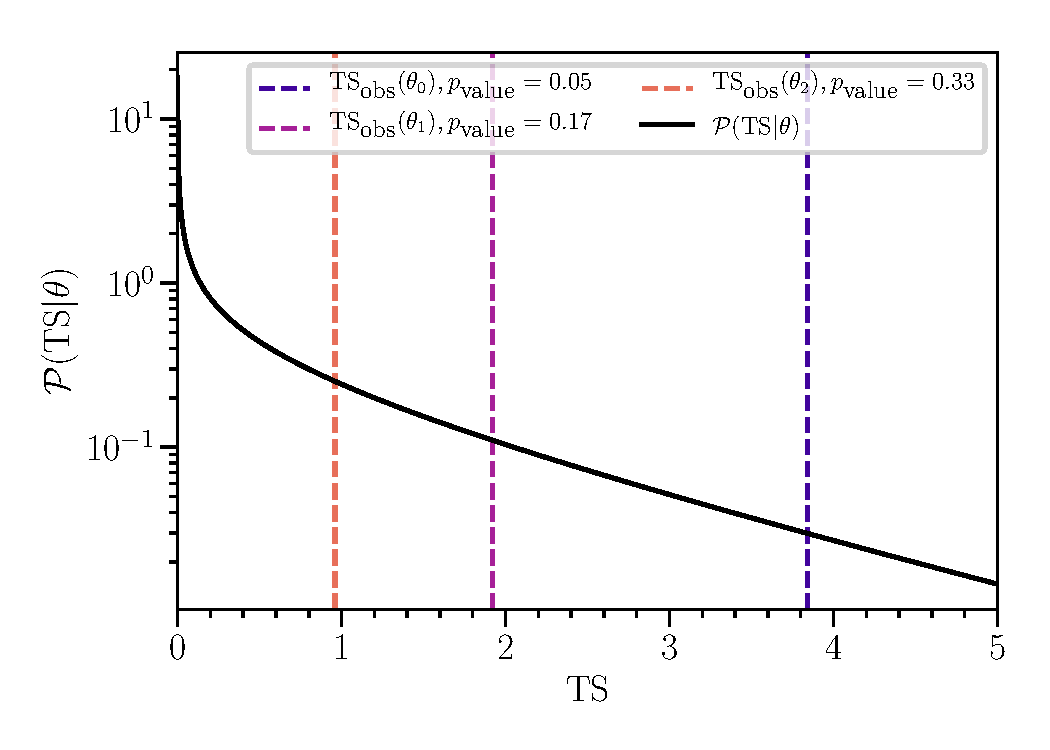
\includegraphics[width=0.8\linewidth]{figures/TS_dist}
	\caption{\textbf{\textit{Test statistic distribution.}} An example of a test statistic distribution.
	Such distributions tend to have the bulk of their mass close to the lower boundary with a long tail.
	Lower values indicate better statistical compatibility with the data.
	}
	\label{fig:TS_dist}
\end{figure}
It is important to note that for the profile likelihood TS and similar statistics a smaller TS value indicates better compatibility with the data.
For this reason many statistical tests are constructed using a single tail significance, by comparing the TS from a single experiment to a background TS distribution and reporting a p-value that is the fraction of the TS distribution greater than the observed TS.

This procedure can be extended to construct intervals by considering the TS distributions of every point in parameter space and comparing to the observed TS function.
Consider the one-dimensional case where there is a TS distribution for each value of the parameter, illustrated in~\reffig{fig:TS_dists_1d}
\begin{figure}
	\centering
	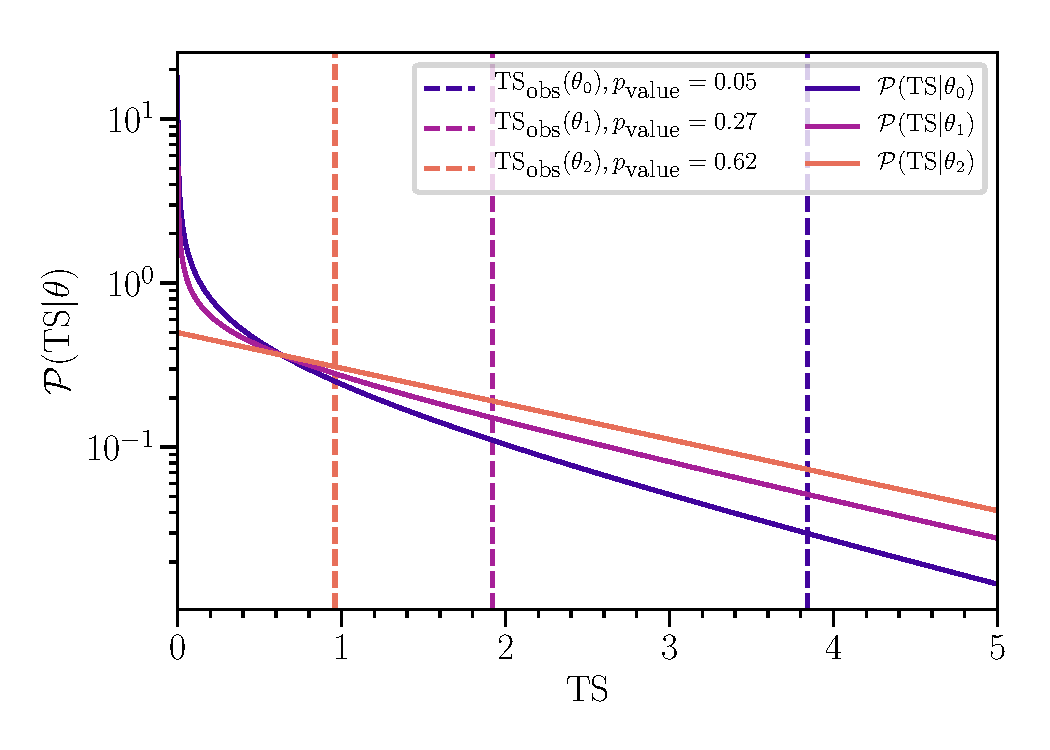
\includegraphics[width=0.8\linewidth]{figures/TS_dists_1d}
	\caption{\textbf{\textit{One-dimensional test-statistic distribution comparison.}} An example of the test statistic distributions as a function of a single parameter.
	}
	\label{fig:TS_dists_1d}
\end{figure}
We can construct an interval that will contain the true value of the parameter a fraction of the time $\alpha$ for repeated experiments.
This interval is the collection of points in the one-dimensional parameter space where the TS at that point is greater than the $\alpha$ quantile of the corresponding TS distribution.
If the TS distribution is the same for all points in parameter space, the interval construction can procedurally be thought of as drawing a horizontal line at the appropriate threshold and only including points that lie below the line.
Varying TS distributions modify this procedure to the comparison of two curves.
This procedure is not limited to one-dimension but can be extended to an arbitrary number of parameters of interest to construct n-dimensional regions with the same properties.

There is however an important caveat to this construction that appears when we consider nuisance parameters.
In order for the intervals to have the desired properties, the observed TS must be greater than the threshold for all possible values of the nuisance parameters.
This ultimatum presents several challenges.
Nuisance parameters can often have a broad or even unbounded range of allowed values, meaning if the effect of nuisance parameters does not taper off at the extrema then almost all intervals are guaranteed to be empty.
From a practical standpoint, computing the TS distributions for many points in parameter space is often done via Monte-Carlo and is computationally expensive.
Adding additional dimensions to the parameter space for which we must compute TS distributions exponentially increases the computation time.

To combat these issues we can limit our interval construction to be valid for values of the nuisance parameters that are ``reasonable''.
There are several methods for doing this, but we can split them into two categories: pure frequentist, and frequentist-Bayesian hybrid.
In the pure frequentist approaches we can either choose a single value of the nuisance parameters, or work with a limited range of the nuisance parameter values.
For the single value approach either nominal values are chosen before looking at the data, or estimators of the nuisance parameters are used to choose their values.
This approach benefits from simplicity, but fails if the test-statistic distributions vary rapidly with changes to the nuisance parameters for values that we might consider ``reasonable''.
A more expensive but robust approach is to explore the behavior of TS distributions for a limited range of the nuisance parameter values, which can be chosen {\it a priori} or from data-based bounds on the nuisance parameters.
If we are willing to consider a hybrid approach, then some more pragmatic options are available.

Although Bayesian methods could be used to choose a single point in parameter space from which to generate the TS distributions, the more interesting application is one that uses a distribution in parameter space.
In Bayesian statistics we can directly assign a probability density to the points in parameter space, either based on our prior information, or directly informed by the posterior distribution, from this extended perspective the probability of certain nuisance parameter values is of interest when considering the frequency of TS values for different parameters of interest.
The prior case is simple in that we sample the from the nuisance parameter priors when generating the TS distribution which allows us to account for variability introduced by the nuisance parameters without relying on hard cutoffs or biasing our inferences with parameter values that are unrealistic.
This prior based technique is well motivated if the priors are derived from external observations, however in the case where nuisance parameters have broad or ``uninformative'' priors this motivation and benefit may break down.
In some cases we expect nuisance parameters to be heavily constrained by the same data sample used to investigate the parameters of interest, so a different approach is merited.
The alternative is to use the posterior distribution to construct our nuisance parameter p.d.f.
Ideally a posterior distribution would be computed for each point in the parameters of interest space by fixing those parameters of interest.
In this way the nuisance parameter posterior used for sampling depends on the point in parameter space we are examining.

With the possible solutions available, we can now look at the problem of limited simulation size when generating test statistic distributions.
As explored in~\refsec{sec:limited_simulation} for binned Poisson likelihood problems, the real expectation in data or simulation for the number of events in a bin is not a known quantity.
Because the real expectations are not known, it is impossible to exactly model the distribution of TS that are expected for a particular point in the parameter space.
However, as~\refsec{sec:limited_simulation} also explored, limited simulation can be modeled with nuisance parameters so the techniques discussed above can be applied directly to the problem.
The ``single point in parameter space'' approach fails to address the additional uncertainty present in this case.
Allowing for unbounded variation of the bin expectations fails as it is guaranteed to produce empty intervals.
Bounding of the bin expectations within a reasonable range provides manageable intervals, but the dimensionality of the problem makes this computationally unfeasible beyond a handful of bins.
Unfortunately this excludes all the ``classic'' frequentist solutions to this problem.
The hybrid Bayesian-frequentist methods in this case provide a tractable solution that accounts for the additional uncertainty.
We can make use of the treatment described in~\refsec{sec:effective}, where the bin expectation is derived to be gamma distributed, and the expected number of data events modeled to be Poisson distributed once this expectation is known.
Practically this can be achieved by sampling data events from $\mcl$, or through a two step process where the expectation is sampled from a gamma distribution $\gprob(\lambda;\agpar, \bgpar)$ where $\agpar = \frac{\mu^2}{\sigma^2}+1~\textmd{and}~\bgpar=\frac{\mu}{\sigma^2}$, and the data events are sampled from a Poisson distribution $\frac{\lambda^{k}e^{-\lambda}}{k!}$.
It is important to note that this procedure only applies to variations in the data and should not be used to vary simulation expectations.
This is because the TS distribution is intended to model variations in the data, whereas the simulation used for analysis is fixed.
Combined with a similar hybrid treatment for other nuisance parameters, this provides a more complete accounting of the uncertainties given the available modeling.
\endgroup

\section{Dealing with limited simulation samples\label{sec:limited_simulation}}
The contents of this section is reproduced here with minor modifications from a collaborative work with Carlos A. Argüelles, and Tianlu Yuan~\cite{Arguelles:2019izp}.

\begingroup
\graphicspath{{results/mcllh_paper/}}
\chapter{Introduction}


\endgroup

\subsection{The Poisson likelihood and previous work\label{sec:mc_intro}}
\begingroup
\graphicspath{{results/mcllh_paper/}}
\input{results/mcllh_paper/sections/previous_work/poisson}
\endgroup

\subsubsection{The Barlow-Beeston likelihood}
\begingroup
\graphicspath{{results/mcllh_paper/}}
\input{results/mcllh_paper/sections/previous_work/bb}
\endgroup

\subsubsection{Uncertainties in the large-sample limit}
\begingroup
\graphicspath{{results/mcllh_paper/}}
\input{results/mcllh_paper/sections/previous_work/chi2}
\endgroup

\subsection{Generalization of the Poisson likelihood\label{sec:generalization_poisson}}
\begingroup
\graphicspath{{results/mcllh_paper/}}
\input{results/mcllh_paper/sections/generalized_poisson/generalized_poisson}
\endgroup

\subsubsection{Derivation of $\like (\lambda|\vecw(\vectheta))$ for identical weights\label{sec:constructing}}
\begingroup
\graphicspath{{results/mcllh_paper/}}
\input{results/mcllh_paper/sections/generalized_poisson/identical_weights}
\endgroup

\subsubsection{Extension to arbitrary weights\label{sec:extending}}
\begingroup
\graphicspath{{results/mcllh_paper/}}
\input{results/mcllh_paper/sections/generalized_poisson/arbitrary_weights}
\endgroup

\subsubsection{The effective likelihood\label{sec:effective}}
\begingroup
\graphicspath{{results/mcllh_paper/}}
\input{results/mcllh_paper/sections/generalized_poisson/effective_likelihood}
\endgroup

\subsubsection{A family of likelihoods\label{sec:priors}}
\begingroup
\graphicspath{{results/mcllh_paper/}}
\input{results/mcllh_paper/sections/generalized_poisson/family}
\endgroup

\subsubsection{Convergence of the effective likelihood\label{sec:llhconvergence}}
\begingroup
\graphicspath{{results/mcllh_paper/}}
\input{results/mcllh_paper/sections/generalized_poisson/convergence}
\endgroup

\subsubsection{Behavior of the effective likelihood\label{sec:llhbehavior}}
\begingroup
\graphicspath{{results/mcllh_paper/}}
\input{results/mcllh_paper/sections/generalized_poisson/behavior}
\endgroup

\subsection{Example and performance\label{sec:example}}
\begingroup
\graphicspath{{results/mcllh_paper/}}
\input{results/mcllh_paper/sections/example/example}
\endgroup

\subsubsection{Point estimation\label{sec:pointestimation}}
\begingroup
\graphicspath{{results/mcllh_paper/}}
\input{results/mcllh_paper/sections/example/point_estimation}
\endgroup

\subsubsection{Coverage\label{sec:coverage}}
\begingroup
\graphicspath{{results/mcllh_paper/}}
\input{results/mcllh_paper/sections/example/coverage}
\endgroup

\subsubsection{Posterior distributions\label{sec:posterior}}
\begingroup
\graphicspath{{results/mcllh_paper/}}
\input{results/mcllh_paper/sections/example/posterior}
\endgroup

\subsubsection{Performance\label{sec:performance}}
\begingroup
\graphicspath{{results/mcllh_paper/}}
\input{results/mcllh_paper/sections/example/performance}
\endgroup

\subsection{Conclusion\label{sec:llhconclusion}}
\begingroup
\graphicspath{{results/mcllh_paper/}}
\input{results/mcllh_paper/sections/conclusion}
\endgroup

\subsection{Summary of likelihood formulas\label{sec:llhtable}}
\begingroup
\graphicspath{{results/mcllh_paper/}}
\input{results/mcllh_paper/appendices/formulas}
\endgroup
\FloatBarrier
\section{Frequentist confidence intervals with nuisance parameters and limited simulation}\label{sec:low_stats_confidence_intervals}

Frequentist and Bayesian techniques deal with different two different kinds of probability.
In frequentist statistics, the relevant probability is the frequency of the outcome of a repeatable experiment.
Under this framework the important concepts are parameter estimation, confidence intervals, and statistical tests.
In Bayesian statistics, the relevant probabilities come from the application of Bayes theorem which means we can define the probability density of parameters.
This definition of the parameter p.d.f. is applicable to the same problems parameter estimation, interval construction, and statistical tests but comes at the cost of defining ``prior belief'' about parameters.

In this section we will ignore the problem of statistical tests, instead focusing on the common features that underpin parameter estimation and interval construction.
Generally in parameter estimation and interval construction there are two sets of parameters, parameters of interest $\vec\theta$ and nuisance parameters $\vec\eta$.
Fundamentally there is no distinction between these two kinds of parameters.
The difference is only in which parameters we want to infer information about.

For both parameter estimation and interval construction the likelihood function is central.
The likelihood function reflects the plausibility of model parameters given observed data and is defined as $\like(\vec\theta, \vec\eta|\textrm{data}) = p(\textrm{data}|\vec\theta, \vec\eta)$.
Where $p(\textrm{data}|\vec\theta, \vec\eta)$ is the probability of the data given the model parameters.
A useful technique to eliminate nuisance parameters is the profile likelihood technique.
Dropping the explicit notational dependence on data, the profile likelihood function is defined as
\begin{linenomath*}
	\begin{equation}
	\tilde{\like}^\texttt{profile}(\vec\theta) = \max_{\vec\eta} \like(\vec\theta,\vec\eta),
	\label{eq:likelihood_profile}
	\end{equation}
\end{linenomath*}
where often the negative log of the function is maximized in place of the function for computational reasons.
The profile likelihood is then only a function of the parameters of interest.
Parameter estimation can be performed by maximizing the profile likelihood to obtain the ``best-fit'' parameters
\begin{linenomath*}
	\begin{equation}
	\hat{\vec\theta} = \argmax_{\vec\theta} \tilde{\like}^\texttt{profile}(\vec\theta).
	\label{eq:best_fit}
	\end{equation}
\end{linenomath*}
This best-fit point in the parameter space is a derived property of the likelihood function.
However, the same procedure can be performed with other functions to the same effect.
In general a minimization procedure is used, and we refer to these functions as ``test-statistics'' (TS).
A particularly useful TS is derived directly from the profile likelihood technique,
\begin{linenomath*}
	\begin{equation}
	\TS(\vec\theta) = -2\log{\left(\frac{\tilde{\like}^\texttt{profile}(\vec\theta)}{\tilde{\like}^\texttt{profile}(\hat{\vec\theta})}\right)}.
	\end{equation}
\end{linenomath*}
Using this TS to perform parameter estimation through minimization is mathematically equivalent to maximizing the likelihood, however, this form will prove to be uniquely useful for interval construction.

Since frequentist statistics deals with the frequency of outcomes from repeated experiments we can use the TS that results from repeated experiments to construct probabilities.
Consider for a moment a single point in the parameter space $\vec\theta_0$.
At this point in the parameter space there is a distribution of data that can be observed, and therefore a distribution of TS functions.
Instead of considering the distribution of TS functions originating from this point, we can simplify the picture by looking at the TS function only evaluated at this point $\TS(\vec\theta_0)$.
This gives us a distribution of TS values for this point in the parameter space that may look like~\reffig{fig:TS_dist}.
\begin{figure}
	\centering
	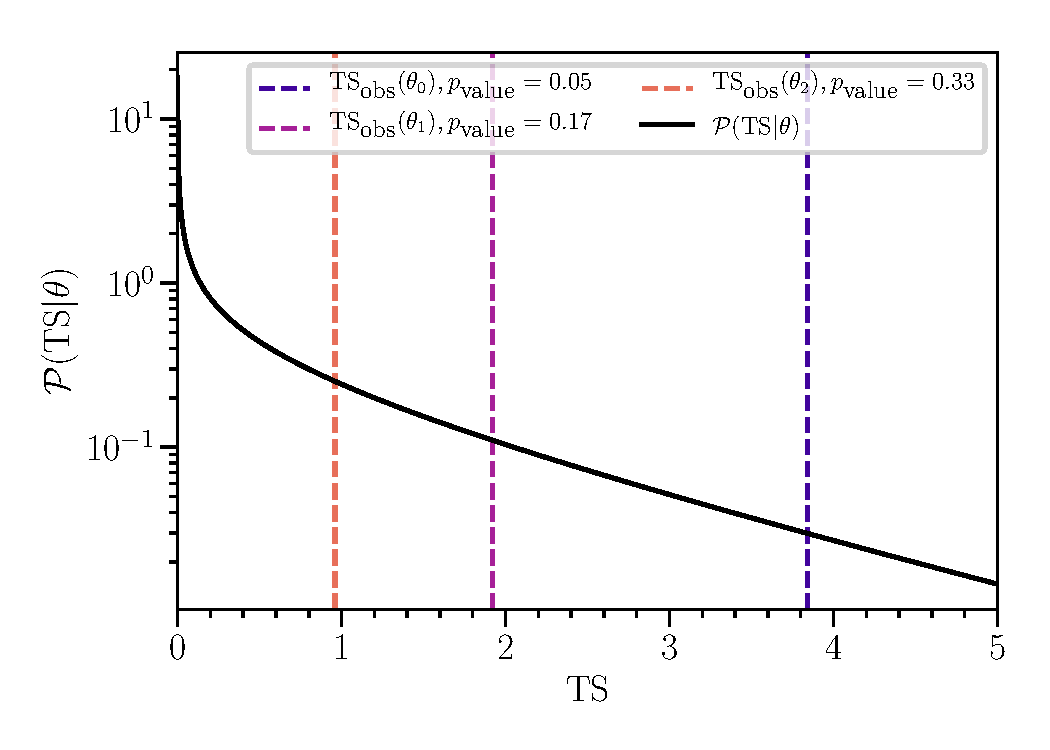
\includegraphics[width=0.8\linewidth]{figures/TS_dist}
	\caption{\textbf{\textit{Test statistic distribution.}} An example of a test statistic distribution.
	Such distributions tend to have the bulk of their mass close to the lower boundary with a long tail.
	Lower values indicate better statistical compatibility with the data.
	}
	\label{fig:TS_dist}
\end{figure}
It is important to note that for the profile likelihood TS and similar statistics a smaller TS value indicates better compatibility with the data.
For this reason many statistical tests are constructed using a single tail significance, by comparing the TS from a single experiment to a background TS distribution and reporting a p-value that is the fraction of the TS distribution greater than the observed TS.

This procedure can be extended to construct intervals by considering the TS distributions of every point in parameter space and comparing to the observed TS function.
Consider the one-dimensional case where there is a TS distribution for each value of the parameter, illustrated in~\reffig{fig:TS_dists_1d}
\begin{figure}
	\centering
	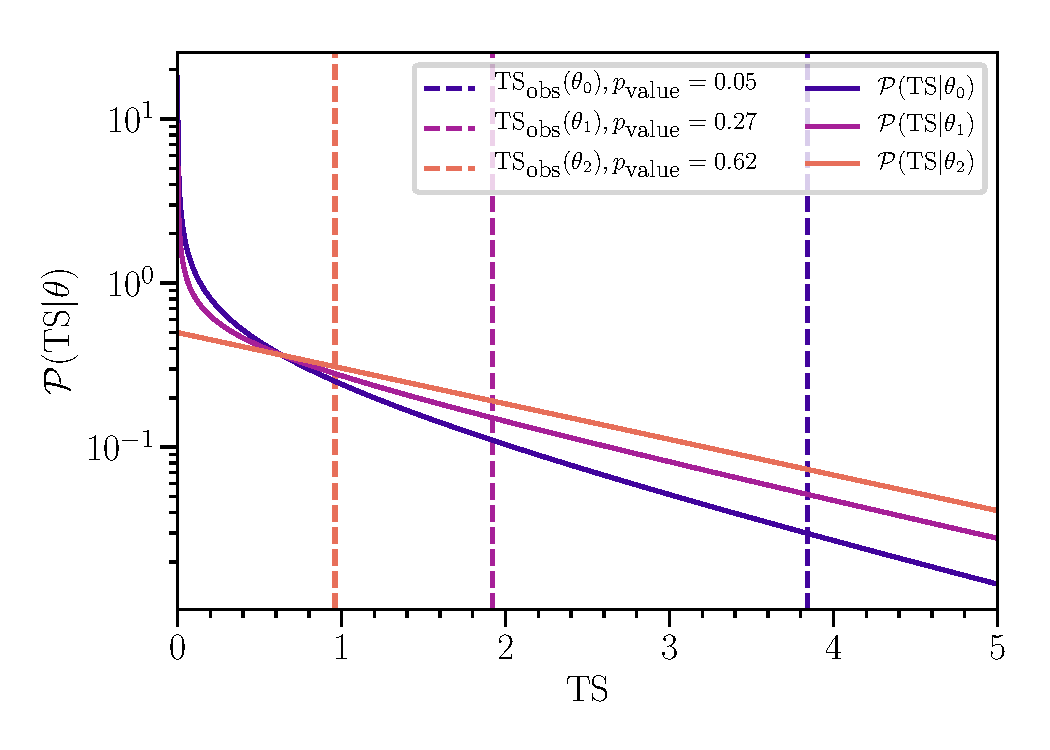
\includegraphics[width=0.8\linewidth]{figures/TS_dists_1d}
	\caption{\textbf{\textit{One-dimensional test-statistic distribution comparison.}} An example of the test statistic distributions as a function of a single parameter.
	}
	\label{fig:TS_dists_1d}
\end{figure}
We can construct an interval that will contain the true value of the parameter a fraction of the time $\alpha$ for repeated experiments.
This interval is the collection of points in the one-dimensional parameter space where the TS at that point is greater than the $\alpha$ quantile of the corresponding TS distribution.
If the TS distribution is the same for all points in parameter space, the interval construction can procedurally be thought of as drawing a horizontal line at the appropriate threshold and only including points that lie below the line.
Varying TS distributions modify this procedure to the comparison of two curves.
This procedure is not limited to one-dimension but can be extended to an arbitrary number of parameters of interest to construct n-dimensional regions with the same properties.

There is however an important caveat to this construction that appears when we consider nuisance parameters.
In order for the intervals to have the desired properties, the observed TS must be greater than the threshold for all possible values of the nuisance parameters.
This ultimatum presents several challenges.
Nuisance parameters can often have a broad or even unbounded range of allowed values, meaning if the effect of nuisance parameters does not taper off at the extrema then almost all intervals are guaranteed to be empty.
From a practical standpoint, computing the TS distributions for many points in parameter space is often done via Monte-Carlo and is computationally expensive.
Adding additional dimensions to the parameter space for which we must compute TS distributions exponentially increases the computation time.

To combat these issues we can limit our interval construction to be valid for values of the nuisance parameters that are ``reasonable''.
There are several methods for doing this, but we can split them into two categories: pure frequentist, and frequentist-Bayesian hybrid.
In the pure frequentist approaches we can either choose a single value of the nuisance parameters, or work with a limited range of the nuisance parameter values.
For the single value approach either nominal values are chosen before looking at the data, or estimators of the nuisance parameters are used to choose their values.
This approach benefits from simplicity, but fails if the test-statistic distributions vary rapidly with changes to the nuisance parameters for values that we might consider ``reasonable''.
A more expensive but robust approach is to explore the behavior of TS distributions for a limited range of the nuisance parameter values, which can be chosen {\it a priori} or from data-based bounds on the nuisance parameters.
If we are willing to consider a hybrid approach, then some more pragmatic options are available.

Although Bayesian methods could be used to choose a single point in parameter space from which to generate the TS distributions, the more interesting application is one that uses a distribution in parameter space.
In Bayesian statistics we can directly assign a probability density to the points in parameter space, either based on our prior information, or directly informed by the posterior distribution, from this extended perspective the probability of certain nuisance parameter values is of interest when considering the frequency of TS values for different parameters of interest.
The prior case is simple in that we sample the from the nuisance parameter priors when generating the TS distribution which allows us to account for variability introduced by the nuisance parameters without relying on hard cutoffs or biasing our inferences with parameter values that are unrealistic.
This prior based technique is well motivated if the priors are derived from external observations, however in the case where nuisance parameters have broad or ``uninformative'' priors this motivation and benefit may break down.
In some cases we expect nuisance parameters to be heavily constrained by the same data sample used to investigate the parameters of interest, so a different approach is merited.
The alternative is to use the posterior distribution to construct our nuisance parameter p.d.f.
Ideally a posterior distribution would be computed for each point in the parameters of interest space by fixing those parameters of interest.
In this way the nuisance parameter posterior used for sampling depends on the point in parameter space we are examining.

With the possible solutions available, we can now look at the problem of limited simulation size when generating test statistic distributions.
As explored in~\refsec{sec:limited_simulation} for binned Poisson likelihood problems, the real expectation in data or simulation for the number of events in a bin is not a known quantity.
Because the real expectations are not known, it is impossible to exactly model the distribution of TS that are expected for a particular point in the parameter space.
However, as~\refsec{sec:limited_simulation} also explored, limited simulation can be modeled with nuisance parameters so the techniques discussed above can be applied directly to the problem.
The ``single point in parameter space'' approach fails to address the additional uncertainty present in this case.
Allowing for unbounded variation of the bin expectations fails as it is guaranteed to produce empty intervals.
Bounding of the bin expectations within a reasonable range provides manageable intervals, but the dimensionality of the problem makes this computationally unfeasible beyond a handful of bins.
Unfortunately this excludes all the ``classic'' frequentist solutions to this problem.
The hybrid Bayesian-frequentist methods in this case provide a tractable solution that accounts for the additional uncertainty.
We can make use of the treatment described in~\refsec{sec:effective}, where the bin expectation is derived to be gamma distributed, and the expected number of data events modeled to be Poisson distributed once this expectation is known.
Practically this can be achieved by sampling data events from $\mcl$, or through a two step process where the expectation is sampled from a gamma distribution $\gprob(\lambda;\agpar, \bgpar)$ where $\agpar = \frac{\mu^2}{\sigma^2}+1~\textmd{and}~\bgpar=\frac{\mu}{\sigma^2}$, and the data events are sampled from a Poisson distribution $\frac{\lambda^{k}e^{-\lambda}}{k!}$.
It is important to note that this procedure only applies to variations in the data and should not be used to vary simulation expectations.
This is because the TS distribution is intended to model variations in the data, whereas the simulation used for analysis is fixed.
Combined with a similar hybrid treatment for other nuisance parameters, this provides a more complete accounting of the uncertainties given the available modeling.
\endgroup

\chapter{Results}

\section{Characterization of the astrophysical neutrino flux\label{sec:diffuse}}
\begingroup
\graphicspath{{results/HESE_Final_Paper/}}
\input{results/HESE_Final_Paper/sections/diffuse/diffuse}
\endgroup

\subsection{Generic models\label{sec:generic_models}}
\begingroup
\graphicspath{{results/HESE_Final_Paper/}}
\input{results/HESE_Final_Paper/sections/diffuse/generic_models}
\endgroup

\subsubsection{Single power-law flux\label{sec:spl}}
\begingroup
\graphicspath{{results/HESE_Final_Paper/}}
\input{results/HESE_Final_Paper/sections/diffuse/spl}
\endgroup

\subsubsection{Double power-law flux\label{sec:dpl}}
\begingroup
\graphicspath{{results/HESE_Final_Paper/}}
\input{results/HESE_Final_Paper/sections/diffuse/dpl}
\endgroup

\subsubsection{Single power law with spectral cutoff\label{sec:cutoff}}
\begingroup
\graphicspath{{results/HESE_Final_Paper/}}
\input{results/HESE_Final_Paper/sections/diffuse/cutoff}
\endgroup

\subsubsection{Log-parabola flux\label{sec:log_parabola}}
\begingroup
\graphicspath{{results/HESE_Final_Paper/}}
\input{results/HESE_Final_Paper/sections/diffuse/lppl}
\endgroup

\subsubsection{Segmented power-law flux\label{sec:unfolding}}
\begingroup
\graphicspath{{results/HESE_Final_Paper/}}
\input{results/HESE_Final_Paper/sections/diffuse/segmented}
\endgroup

\subsection{Atmospheric flux from charmed hadrons\label{sec:prompt}}
\begingroup
\graphicspath{{results/HESE_Final_Paper/}}
\input{results/HESE_Final_Paper/sections/diffuse/prompt}
\endgroup

\subsection{Source-specific models\label{sec:specific_models}}
\begingroup
\graphicspath{{results/HESE_Final_Paper/}}
\input{results/HESE_Final_Paper/sections/diffuse/specific_models}
\endgroup

\bibliographystyle{ieeetr}
\bibliography{results/HESE_Final_Paper/hesebiblio,results/mcllh_paper/likelihood,thesis-citations}

\clearpage
\newpage
\appendix

\chapter{Appendix}
\begingroup
\graphicspath{{results/HESE_Final_Paper/}}
\section{High-energy astrophysical neutrino source searches\label{sec:sources}}
\subfile{results/HESE_Final_Paper/sections/sources}
\section{Expected number of events table\label{sec:events_table}}
\subfile{results/HESE_Final_Paper/appendices/event_table}
\section{Event comparison\label{sec:comparison}}
\subfile{results/HESE_Final_Paper/appendices/comparison}
\section{Source catalog\label{sec:source_catalog}}
\subfile{results/HESE_Final_Paper/appendices/sources_table}
\section{Sideband distributions\label{sec:sidebands}}
\subfile{results/HESE_Final_Paper/appendices/sidebands}
\section{Effects of systematics in analysis distributions\label{sec:extendedsys}}
\subfile{results/HESE_Final_Paper/appendices/extendedsys}
\section{Single photo-electron charge distribution calibration\label{sec:charge_calibration}}
\subfile{results/HESE_Final_Paper/appendices/charge_calibration}
\section{Detailed likelihood description\label{sec:likelihood}}
\subfile{results/HESE_Final_Paper/appendices/likelihood}
\section{Data release for additional characterization of the astrophysical neutrino flux\label{sec:release}}
\subfile{results/HESE_Final_Paper/appendices/release}
\endgroup

\end{document}
